% !TeX program = xelatex
%% Formatted according to the SEEP2026 proceedings template
%% (Tor Vergata University, Rome, 20-23 July 2026).
%% NOTE: this file must be compiled with XeLaTeX (or LuaLaTeX),
%% because it uses the real Arial / Arial Narrow / Times New Roman fonts
%% required by the template. It will NOT compile with pdfLaTeX.
\documentclass[12pt,a4paper]{article}

% ---------- Type area ----------
\usepackage[a4paper,top=2cm,bottom=2cm,left=2.5cm,right=2.5cm,%
            headsep=0.6cm,includehead]{geometry}

% ---------- Math ----------
\usepackage{amsmath}

% ---------- Fonts (template-specified) ----------
\usepackage{fontspec}
\setmainfont{Times New Roman}                 % Body text, affiliation, header
\newfontfamily\arialfont{Arial}               % Headings, authors, captions
\newfontfamily\arialnarrow{Arial Narrow}      % Paper title

% Times-consistent math (digits, upright and symbols), integrated with fontspec.
% Replaces newtxmath, which under XeLaTeX let math digits fall back to Latin Modern.
\usepackage{unicode-math}
\setmathfont{texgyretermes-math.otf}          % Times-clone math font

% ---------- Graphics ----------
\usepackage{graphicx}
\usepackage{subcaption}

% ---------- Running header (every page), no page numbers ----------
\usepackage{fancyhdr}
\newcommand{\seepheader}{\itshape Proceedings of SEEP2026, 20-23 July 2026,%
\ Tor Vergata University, Rome, Italy}
\pagestyle{fancy}
\fancyhf{}
\setlength{\headheight}{14.5pt}
\renewcommand{\headrulewidth}{0pt}
\fancyhead[L]{\normalfont\fontsize{12}{14}\selectfont\seepheader}
\fancypagestyle{plain}{%
  \fancyhf{}%
  \renewcommand{\headrulewidth}{0pt}%
  \fancyhead[L]{\normalfont\fontsize{12}{14}\selectfont\seepheader}%
}
\pagenumbering{gobble}            % no page numbers

% ---------- Section headings (Heading 1/2/3 styles) ----------
\usepackage{titlesec}
\setcounter{secnumdepth}{2}       % third-order headings are NOT numbered

% Heading 1: Arial, bold, 12pt, ALL CAPS, left, numbered
\titleformat{\section}
  {\arialfont\bfseries\fontsize{12}{14}\selectfont}
  {\thesection}{0.8em}{\MakeUppercase}
% Heading 2: Arial, bold, 12pt, left, numbered
\titleformat{\subsection}
  {\arialfont\bfseries\fontsize{12}{14}\selectfont}
  {\thesubsection}{0.8em}{}
% Heading 3: Arial, italic, 12pt, left, NOT numbered
\titleformat{\subsubsection}
  {\arialfont\itshape\fontsize{12}{14}\selectfont}
  {}{0pt}{}
\titlespacing*{\section}      {0pt}{12pt}{6pt}
\titlespacing*{\subsection}   {0pt}{10pt}{4pt}
\titlespacing*{\subsubsection}{0pt}{8pt}{2pt}

% ---------- Captions (Figure/Table Heading: Arial, 12pt, centered, per template) ----------
\usepackage{caption}
\DeclareCaptionFont{arial}{\arialfont\fontsize{12}{14}\selectfont}
\captionsetup{font=arial,labelfont=arial,labelsep=period,%
              justification=centering,singlelinecheck=true}

% ---------- Abstract: "ABSTRACT" centered, bold, Arial ----------
\renewenvironment{abstract}{%
  \begin{center}%
    {\arialfont\bfseries\fontsize{12}{14}\selectfont ABSTRACT}%
  \end{center}%
  \par\noindent\ignorespaces
}{\par\vspace{6pt}}

% ---------- Keywords command ----------
\newcommand{\keywords}[1]{\par\noindent{\itshape Keywords}: #1\par\vspace{6pt}}

\begin{document}

%%% TITOLO, AUTORI, AFFILIAZIONE (Title block per template SEEP2026)
\begin{center}
  {\arialnarrow\bfseries\fontsize{14}{17}\selectfont
   \MakeUppercase{CFD-ML-Based Turbulence Model Definition for Fidelity
   Improvement of Horizontal-Axis Wind Turbine RANS Simulations}\par}
  \vspace{6pt}
  {\arialfont\bfseries\fontsize{12}{14}\selectfont Andrea Carloni\textsuperscript{1}\par , Giovanni Delibra\textsuperscript{2}\par, Filippo De Girolamo\textsuperscript{3}\par, Lorenzo Tieghi\textsuperscript{4}\par, Alessandro Corsini\textsuperscript{2}\par, Valerio Francesco Barnabei\textsuperscript{2}\par}
  \vspace{2pt}
  {\fontsize{12}{14}\selectfont
   1.\ Department of Electrical and Energy Engineering, Sapienza University
   of Rome, Italy; email: andrea.carloni@uniroma1.it\par}
  {\fontsize{12}{14}\selectfont
   2.\ Department of Mechanical and Aerospace Engineering, Sapienza University
   of Rome, Italy; email: giovanni.delibra@uniroma1.it\par}
  {\fontsize{12}{14}\selectfont
   3.\ Division of Fluid Mechanics, KTH Royal Institute of Technology, Stockholm, Sweden; email:fidg@kth.se\par}
  {\fontsize{12}{14}\selectfont
   4.\ Department of Civil, Environmental and Mechanical Engineering, University of Trento, Trento, Italy; email: lorenzo.tieghi@unitn.it\par}

\end{center}
\vspace{6pt}

%%%abstract
\begin{abstract}
Accurate prediction of horizontal-axis wind turbine (HAWT) wakes is
essential for wind farm layout optimisation, energy-yield estimation and
load assessment, yet it remains a major challenge for affordable
simulation tools. Large Eddy Simulation (LES) reproduces the wake physics
reliably but at a prohibitive computational cost, whereas unsteady
Reynolds-Averaged Navier-Stokes (URANS) closures systematically
mis-predict the wake recovery because of the assumptions embedded in the
eddy-viscosity hypothesis. This work proposes a CFD-ML methodology that
uses machine learning to \emph{define}, rather than post-process, the
turbulence closure of a $k$-$\omega$ SST RANS solver for HAWT wakes.
From a single high-fidelity LES of the NREL-5MW turbine operating in a
turbulent atmospheric boundary layer (ABL), an LES-equivalent
eddy-viscosity field $\nu_{t,eq}$ is extracted and used as the regression
target. A K-means clustering algorithm first segments the flow into
physically distinct regions, and a Multi-Layer Perceptron (MLP) is then
trained to predict the local correction $\Delta\nu_t = \nu_{t,eq} -
\nu_{t,\mathrm{RANS}}$. The resulting closure is embedded directly into a
modified OpenFOAM PIMPLE solver and evaluated in a fully predictive
setting. By design, the closure is calibrated on this single reference
case and then transferred, without retraining, to grid resolutions and
inflow velocities never seen during training: this single-case-to-many
transfer is the core premise of the methodology, not a limitation of it.
The trained network reproduces the LES-equivalent eddy viscosity with a
validation coefficient of determination $R^2 = 0.9952$, and the
clustering step is shown to improve the reconstruction in the
near-terrain region. Once embedded in the solver, the ML-based closure
consistently outperforms the standard RANS model in both the near- and
far-wake and remains close to the LES reference at the unseen inflow
velocities of $8$ and $15\,\mathrm{m/s}$. Most notably, on ultra-coarse
grids the model accurately captures the post-breakdown wake recovery at a
computational cost about $1.25$ times lower than the reference LES, while
also reproducing the rotor forces and power coefficients. These results
indicate that a turbulence closure trained once on an affordable amount
of high-fidelity data can deliver LES-quality wake predictions at a cost
compatible with practical wind farm applications.
\end{abstract}

\keywords{Wind turbine wake, URANS, Machine learning, Turbulence modelling, LES, CFD, Clustering, Neural Networks}

%%%nomenclature
\section*{Nomenclature}
$\vec{U}$             velocity field [m/s] \\
$\vec{U}_{cyl}$       velocity field in cylindrical coordinates, $(U_x, U_\theta, U_\rho)$ [m/s] \\
$U_{ref}$            reference inflow velocity at hub height [m/s] \\
$U_\theta$           tangential velocity component [m/s] \\
$U_\rho$             radial velocity component [m/s] \\
$p$                  kinematic pressure [m$^2$/s$^2$] \\
$k$                  turbulent kinetic energy [m$^2$/s$^2$] \\
$D$                  rotor diameter [m] \\
$z$                  vertical coordinate from the ground [m] \\
$z_0$                aerodynamic roughness length [m] \\
$z_{ref}$            reference (hub) height [m] \\
$x/D,\; z/D$         streamwise and vertical coordinates normalised by the rotor diameter [-] \\
$S_{ij}$             resolved strain-rate tensor [1/s] \\
$R_{ij}^{res}$       resolved Reynolds stress tensor [m$^2$/s$^2$] \\
$Q$                  second invariant of the velocity gradient tensor (Q-criterion) [1/s$^2$] \\
$\mathbf{R}$         Reynolds stress tensor [m$^2$/s$^2$] \\
$C_p,\; C_t$         power and thrust coefficients [-] \\
$\epsilon$           Gaussian projection width of the ALM body force [m] \\
$\Delta x$           cell size [m] \\
$\Delta b$           actuator-line element spacing [m] \\
$\Delta t$           simulation time step [s] \\
$R^2$                coefficient of determination [-] \\
$\mathrm{Inertia}$   within-cluster sum of squares (WCSS) minimised by K-means [-] \\
$K$                  number of clusters [-] \\
$C_i,\; \mu_i$       set of points and centroid of cluster $i$ [-] \\
$w_{ax}$             axial sample weight in the NN loss [-] \\
$n_0,\; n_i,\; r$    initial neuron width, width of layer $i$, width-decay factor [-] \\[6pt]
$\nu$                molecular kinematic viscosity [m$^2$/s] \\
$\nu_{eff}$          effective kinematic viscosity, $\nu+\nu_t$ [m$^2$/s] \\
$\nu_t$              turbulent (eddy) kinematic viscosity [m$^2$/s] \\
$\nu_{t,\mathrm{RANS}}$ baseline RANS eddy viscosity [m$^2$/s] \\
$\nu_{t,eq}$         LES-equivalent eddy viscosity (regression target reference) [m$^2$/s] \\
$\nu_{t,mod}$        modified eddy viscosity reproducing the LES mean fields [m$^2$/s] \\
$\nu_{t,ML}$         ML-reconstructed eddy viscosity, $\nu_{t,\mathrm{RANS}}+\Delta\nu_{t,ML}$ [m$^2$/s] \\
$\nu_{sgs}$          subgrid-scale eddy viscosity [m$^2$/s] \\
$\Delta\nu_t$        eddy-viscosity correction, $\nu_{t,eq}-\nu_{t,\mathrm{RANS}}$ [m$^2$/s] \\
$\tau_{ij}^{sgs}$    subgrid-scale stress tensor [m$^2$/s$^2$] \\
$\Sigma_{ij}^{dev}$  deviatoric part of the total turbulent stress tensor [m$^2$/s$^2$] \\
$\omega$             specific turbulence dissipation rate [1/s] \\
$\delta$             Huber-loss transition parameter [-] \\[6pt]

\textbf{Acronyms} \\
ABL                  Atmospheric Boundary Layer \\
ALM                  Actuator Line Model \\
CA                   Clustering Algorithm \\
CFD                  Computational Fluid Dynamics \\
FIML                 Field Inversion and Machine Learning \\
GELU                 Gaussian Error Linear Unit \\
HAWT                 Horizontal-Axis Wind Turbine \\
LES                  Large Eddy Simulation \\
MAE                  Mean Absolute Error \\
ML                   Machine Learning \\
MLP                  Multi-Layer Perceptron \\
MSE                  Mean Squared Error \\
NN                   Neural Network \\
NREL                 National Renewable Energy Laboratory \\
PCA                  Principal Component Analysis \\
PC                   Principal Component \\
RANS                 Reynolds-Averaged Navier-Stokes \\
RMSE                 Root Mean Squared Error \\
SCADA                Supervisory Control And Data Acquisition \\
SGS                  Subgrid-Scale \\
SST                  Shear-Stress Transport \\
WALE                 Wall-Adapting Local Eddy-viscosity \\
WCSS                 Within-Cluster Sum of Squares \\
WT                   Wind Turbine \\

%%%introduction
\section{Introduction}
\label{introduction}
%%% intro problema fisico: perché è difficile predirre il comportamento delle scie eoliche? perché è importante riuscire a farlo? spiega natura del fenomeno e difficoltà di modellizzazione
%%% Spiega che esistono diverse tecniche per modellizzare le scie eoliche, ma che tutte hanno dei limiti (o fedeltà o costo computazionale).
%%% cita l uso di tecniche di machine learning in campo eolico per la predizione della potenza, gestione manutentiva, ottimizzazione del layout
%%% spiega che in questo lavoro ci si concentra su un approccio di machine learning per la predizione del comportamento delle scie eoliche, quindi un qualcosa di diverso rispetto a quanto visto perché "si tratta proprio di creare da zero un modello di turbolenza ML-based" e non di usare un modello di turbolenza esistente per predire la potenza o ottimizzare il layout e poi usare tecniche di ML per migliorare la predizione o usarle in post sulla base di quei risultati per ottimizzare il layout o la gestione manutentiva.
%%% fai esempi di lavori che hanno usato tecniche di ML per predire la potenza o ottimizzare il layout e anche di lavori che hanno usato tecniche di ML per migliorare la predizione dei modelli di turbolenza esistenti. 
%%% spiega che questo approccio è interessante perché potrebbe permettere di superare i limiti dei modelli di turbolenza tradizionali, che spesso non riescono a catturare la complessità del fenomeno eolico, e potrebbe portare a predizioni più accurate e a una migliore comprensione del comportamento delle scie eoliche nonché a una possibile futura applicazione in real time con il funzionamento della farm attraveso la possibilità di ottenere modelli rappresentiativi compatti del campo e del suo funzionamento. 
Wind energy is one of the cornerstones of the ongoing transition toward sustainable electricity generation. As wind turbines are deployed in increasingly large farms, both onshore and offshore, the aerodynamic interaction among turbines becomes a critical design and operational challenge. When a turbine extracts kinetic energy from the incoming flow, it leaves behind a wake region characterised by a significant velocity deficit and elevated turbulence levels. Downstream turbines that operate within this region consequently suffer both reduced power output and increased fatigue loads, affecting the economic and structural performance of the entire farm~\cite{Porte-Agel2020}. Accurate prediction of wind turbine wake behaviour is therefore essential for wind farm layout optimisation, energy yield estimation, and structural load assessment.

From a fluid-mechanics perspective, the wake of a horizontal-axis wind turbine (HAWT) is a complex, multi-scale phenomenon. It is deeply coupled with the Atmospheric Boundary Layer (ABL), which is itself inherently unsteady and stratified~\cite{Porte-Agel2020}. The near-wake region, dominated by the tip vortex system shed by the rotor blades, transitions into a far-wake where shear-driven turbulent mixing progressively restores the velocity deficit. This recovery process is strongly influenced by the ambient turbulence intensity, wind shear, thermal stability, and the topography of the terrain~\cite{heck2025unravelingeffectsatmosphericdynamics}. The wide range of length and time scales involved, from blade boundary layers to the full extent of the ABL, makes any single simulation approach inherently challenging.

Several modelling strategies are available, each representing a different trade-off between physical fidelity and computational cost. On one end of the spectrum, analytical engineering wake models (e.g., the Jensen top-hat model and its Gaussian successors) offer near-instantaneous evaluation and are therefore routinely used in wind farm layout optimisation~\cite{GholamiAnjiraki2025}, but they rely on strong simplifying assumptions and cannot capture the complex turbulent structure of real wakes. On the other end, Large Eddy Simulation (LES) resolves the dominant turbulent structures explicitly and is considered the reference standard for wake physics; however, a single simulation of a medium-sized wind farm can demand between $10^5$ and $3 \times 10^6$ CPU hours~\cite{Steiner2021}, making it prohibitively expensive for systematic design or optimisation studies. Unsteady Reynolds-Averaged Navier-Stokes (URANS) methods occupy an intermediate position, reducing computational cost by roughly two orders of magnitude relative to LES~\cite{Steiner2021}. Yet the closure assumptions embedded in standard RANS turbulence models, most notably the Boussinesq eddy-viscosity hypothesis and the isotropic treatment of the Reynolds stress tensor, introduce structural model-form errors that are particularly pronounced in separated and wake flows, leading to a systematic mis-prediction of the wake recovery rate~\cite{72116acdc5aa4b3b8fc752f1b2fa9958,Moss2023}.

Machine Learning (ML) has emerged as a powerful paradigm to complement or enhance physics-based simulations across several domains of wind energy research. A large body of literature has applied ML to operational tasks such as wind power forecasting from SCADA data~\cite{Infield2022,Moss2023}, predictive maintenance and condition monitoring of turbine components~\cite{Infield2022}, and wind farm layout optimisation using data-driven surrogate models of wake interactions~\cite{GholamiAnjiraki2025,YANG2023119240}. In these applications ML is generally used downstream of a physical model: a CFD or analytical solver first generates the flow field, and ML then post-processes or surrogate-replaces its output to predict power, loads, or optimal configurations. 

A conceptually distinct and more recent line of research aims instead to use ML to correct or replace the turbulence closure itself, modifying the governing equations during the simulation. An example of that can be seen in ~\cite{Duraisamy2019} with the proposed FIML (field inversion and machine learning) proposed by Parish \& Duraisamy and the invariant neural-network closure of Ling et al.~\cite{Ling2016}. In the wind energy context, Steiner et al.~\cite{Steiner2021} demonstrated that optimal corrective fields for the turbulence anisotropy tensor and turbulent kinetic energy production can be derived from time-averaged LES data and used to construct a custom RANS closure via sparse symbolic regression, yielding substantially improved wake predictions for multi-turbine configurations at wind-tunnel scale. Similarly, data-driven Gaussian-process corrections to the eddy-viscosity field, trained on single-turbine LES, have shown improved accuracy when deployed in a wind-plant RANS simulation~\cite{King_2018}. More broadly, Steiner~\cite{72116acdc5aa4b3b8fc752f1b2fa9958} showed that combined baseline-RANS plus data-driven correction strategies can outperform standard models for both velocity and turbulent kinetic energy, while acknowledging that larger datasets and more stable numerical implementations are needed before such methods can be applied at industrial scale.

The present work contributes to this emerging research direction, with specific novelty in three respects. First, rather than identifying a global correction to the turbulence model, a clustering algorithm (CA) based on the K-means method is employed to segment the flow domain into physically distinct regions characterised by different wake dynamics, following the decomposition approach introduced in~\cite{Clustering_tieghi,Carloni2026}. This region-aware strategy naturally improves the generalisability and interpretability of the trained models and makes the correction less sensitive to mesh refinement. Second, a Multi-Layer Perceptron (MLP) is trained to predict the local correction $\Delta\nu_t = \nu_{t,eq} - \nu_{t,\mathrm{RANS}}$ between the LES-equivalent eddy viscosity and the RANS baseline, and the resulting data-driven closure is directly embedded into the OpenFOAM PIMPLE solver via a modified turbulence correction loop, enabling its use in fully predictive RANS simulations. Third, the methodology is tested across multiple mesh refinement levels, demonstrating that LES-quality accuracy in wake recovery can be achieved at a computational cost lower than that of standard LES, which is a prerequisite for practical wind farm applications.

It is worth emphasising what distinguishes this approach from the bulk of ML applications in wind energy. Most existing methods employ ML as a post-processing or surrogate tool applied to the output of a turbulence model; the turbulence model itself is left unchanged. Here, the ML component is used to define the turbulence model, to construct, from scratch, a problem-specific eddy-viscosity closure calibrated to reproduce high-fidelity LES statistics. This opens a path towards compact, computationally efficient flow models that could in the future support real-time wind farm monitoring and control, by providing accurate yet computational effective representations of the wake field and its evolution under varying inflow conditions.

The paper is structured as follows. Sec.~\ref{sec:methodology} describes the CFD campaign used to generate the training and testing data, the clustering pipeline, and the MLP architecture and training strategy. Sec.~\ref{sec:case_study} introduces the NREL-5MW reference turbine case study and the computational domain. Results are presented in Sec.~\ref{sec:results}, covering the clustering, the neural network training metrics, and the performance of the ML-based RANS model on coarser grids. Conclusions are drawn in Sec.~\ref{sec:conclusions}.

%%%methodology
\section{Methodology}
\label{sec:methodology}
The methodology adopted relies both, as cited, on a CFD and on a ML part. The CFD part is used to generate the data and test the model while the ML part is used to train the models, both Clustering and NN.

\subsection{CFD dataset}

A CFD simulation campaign is performed to generate the data for the ML part.
Simulations are performed via OpenFOAM-v22.12, an open-source CFD software including an in-house implementation of Actuator Line Model (ALM)\cite{10.1115/1.1471361} based on the open-source library \textit{turbinesFoam}\cite{turbinesFoam}. Both RANS and LES simulations are performed, assuming incompressible flow conditions.
$\vec{U}$ and $p$ fields are solved with the PIMPLE algorithm.
In all the simulations the timestep, corresponding to $2^\circ$ of rotation of the WT rotor, is set to ensure a maximum Courant number of 0.6 with a mean value of 0.02-0.03, while the time integration relied on a first-order Euler scheme. Second order central differences were used for the spatial discretisation of the convective and diffusive terms.

The RANS simulations are performed with the $k$-$\omega$ SST turbulence model \cite{doi:10.2514/3.12149} while the LES simulations are performed with the WALE turbulence model \cite{WALE}.

The following boundary conditions were applied in the RANS case: at the inlet a logarithmic velocity profile was imposed. At the outlet, a zero-gradient condition was set
for the $\vec{U}$ field. No-slip boundary conditions were set for the ground, while freestream conditions were applied to the other lateral boundaries. For pressure a zero-gradient condition was set for all the boundaries.

In the LES case, the same boundary conditions were applied except for the inlet $\vec{U}$ field, where turbulent fluctuations, derived from the Kaimal spectrum, were superimposed to the logarithmic velocity profile. Synthetic inflow conditions based on a spectra-stochastic method are imposed at the inlet derived from the Kaimal power spectral density function \cite{kaimal} following the approach described in \cite{Davidson2007UsingIS}. As done in \cite{Carloni2026}, the turbulent fluctuations are generated by a coded boundary condition, imposing a total of 400 Fourier modes. Continuity is ensured by constraining the orthogonality of the wave numbers and $\vec{U}$. Spatial coherence is imposed through an exponential decay function $\exp(\frac{-\Delta t}{T})$ where $\Delta t$ is the time step of the simulations and $T$ is the time scale of the turbulence considered.

Moreover, to generate the data for the ML regression, a dedicated RANS run was set up by importing the time-averaged $\vec{U}$ and $p$ fields from the LES. Keeping these mean fields frozen, a single iteration of the turbulence-correction loop was then performed, so that the eddy-viscosity field is solved consistently with the imposed LES mean fields, yielding the modified eddy viscosity field $\nu_{t,mod}$. This frozen-field procedure returns, on the RANS grid and within the RANS solver, the eddy-viscosity distribution that the baseline closure would require in order to be consistent with the LES mean flow, and provides the reference against which the data-driven correction is later assessed.

All the model training and testing is performed on the same computational domain, which is a rectangular box where the rotor is placed at 5D from the inlet and 15D from the outlet and $90 m$ from terrain. In spanwise direction the domain extends for 5D on each side of the rotor and in normal direction 8D from the ground.
The domain is obtained by using the \textit{blockMesh} and \textit{snappyHexMesh} utilities of OpenFOAM, with different refinement levels in different regions of the domain to proper solve the turbulent structures in the near wake of the rotor.
Moreover, an inflation layer is applied near terrain. The final mesh consists of around $\sim30.8$ million cells with a minimum cell size of 1.75 m near the rotor and a maximum cell size of 28 m at the domain boundaries while reaching $\sim0.33$ m in the first level of the inflation layer near the ground.
In Fig.~\ref{fig:mesh} the computational domain and the mesh refinement are shown.
\begin{figure*}[h]
    \centering
    \begin{subfigure}[b]{0.49\textwidth}
        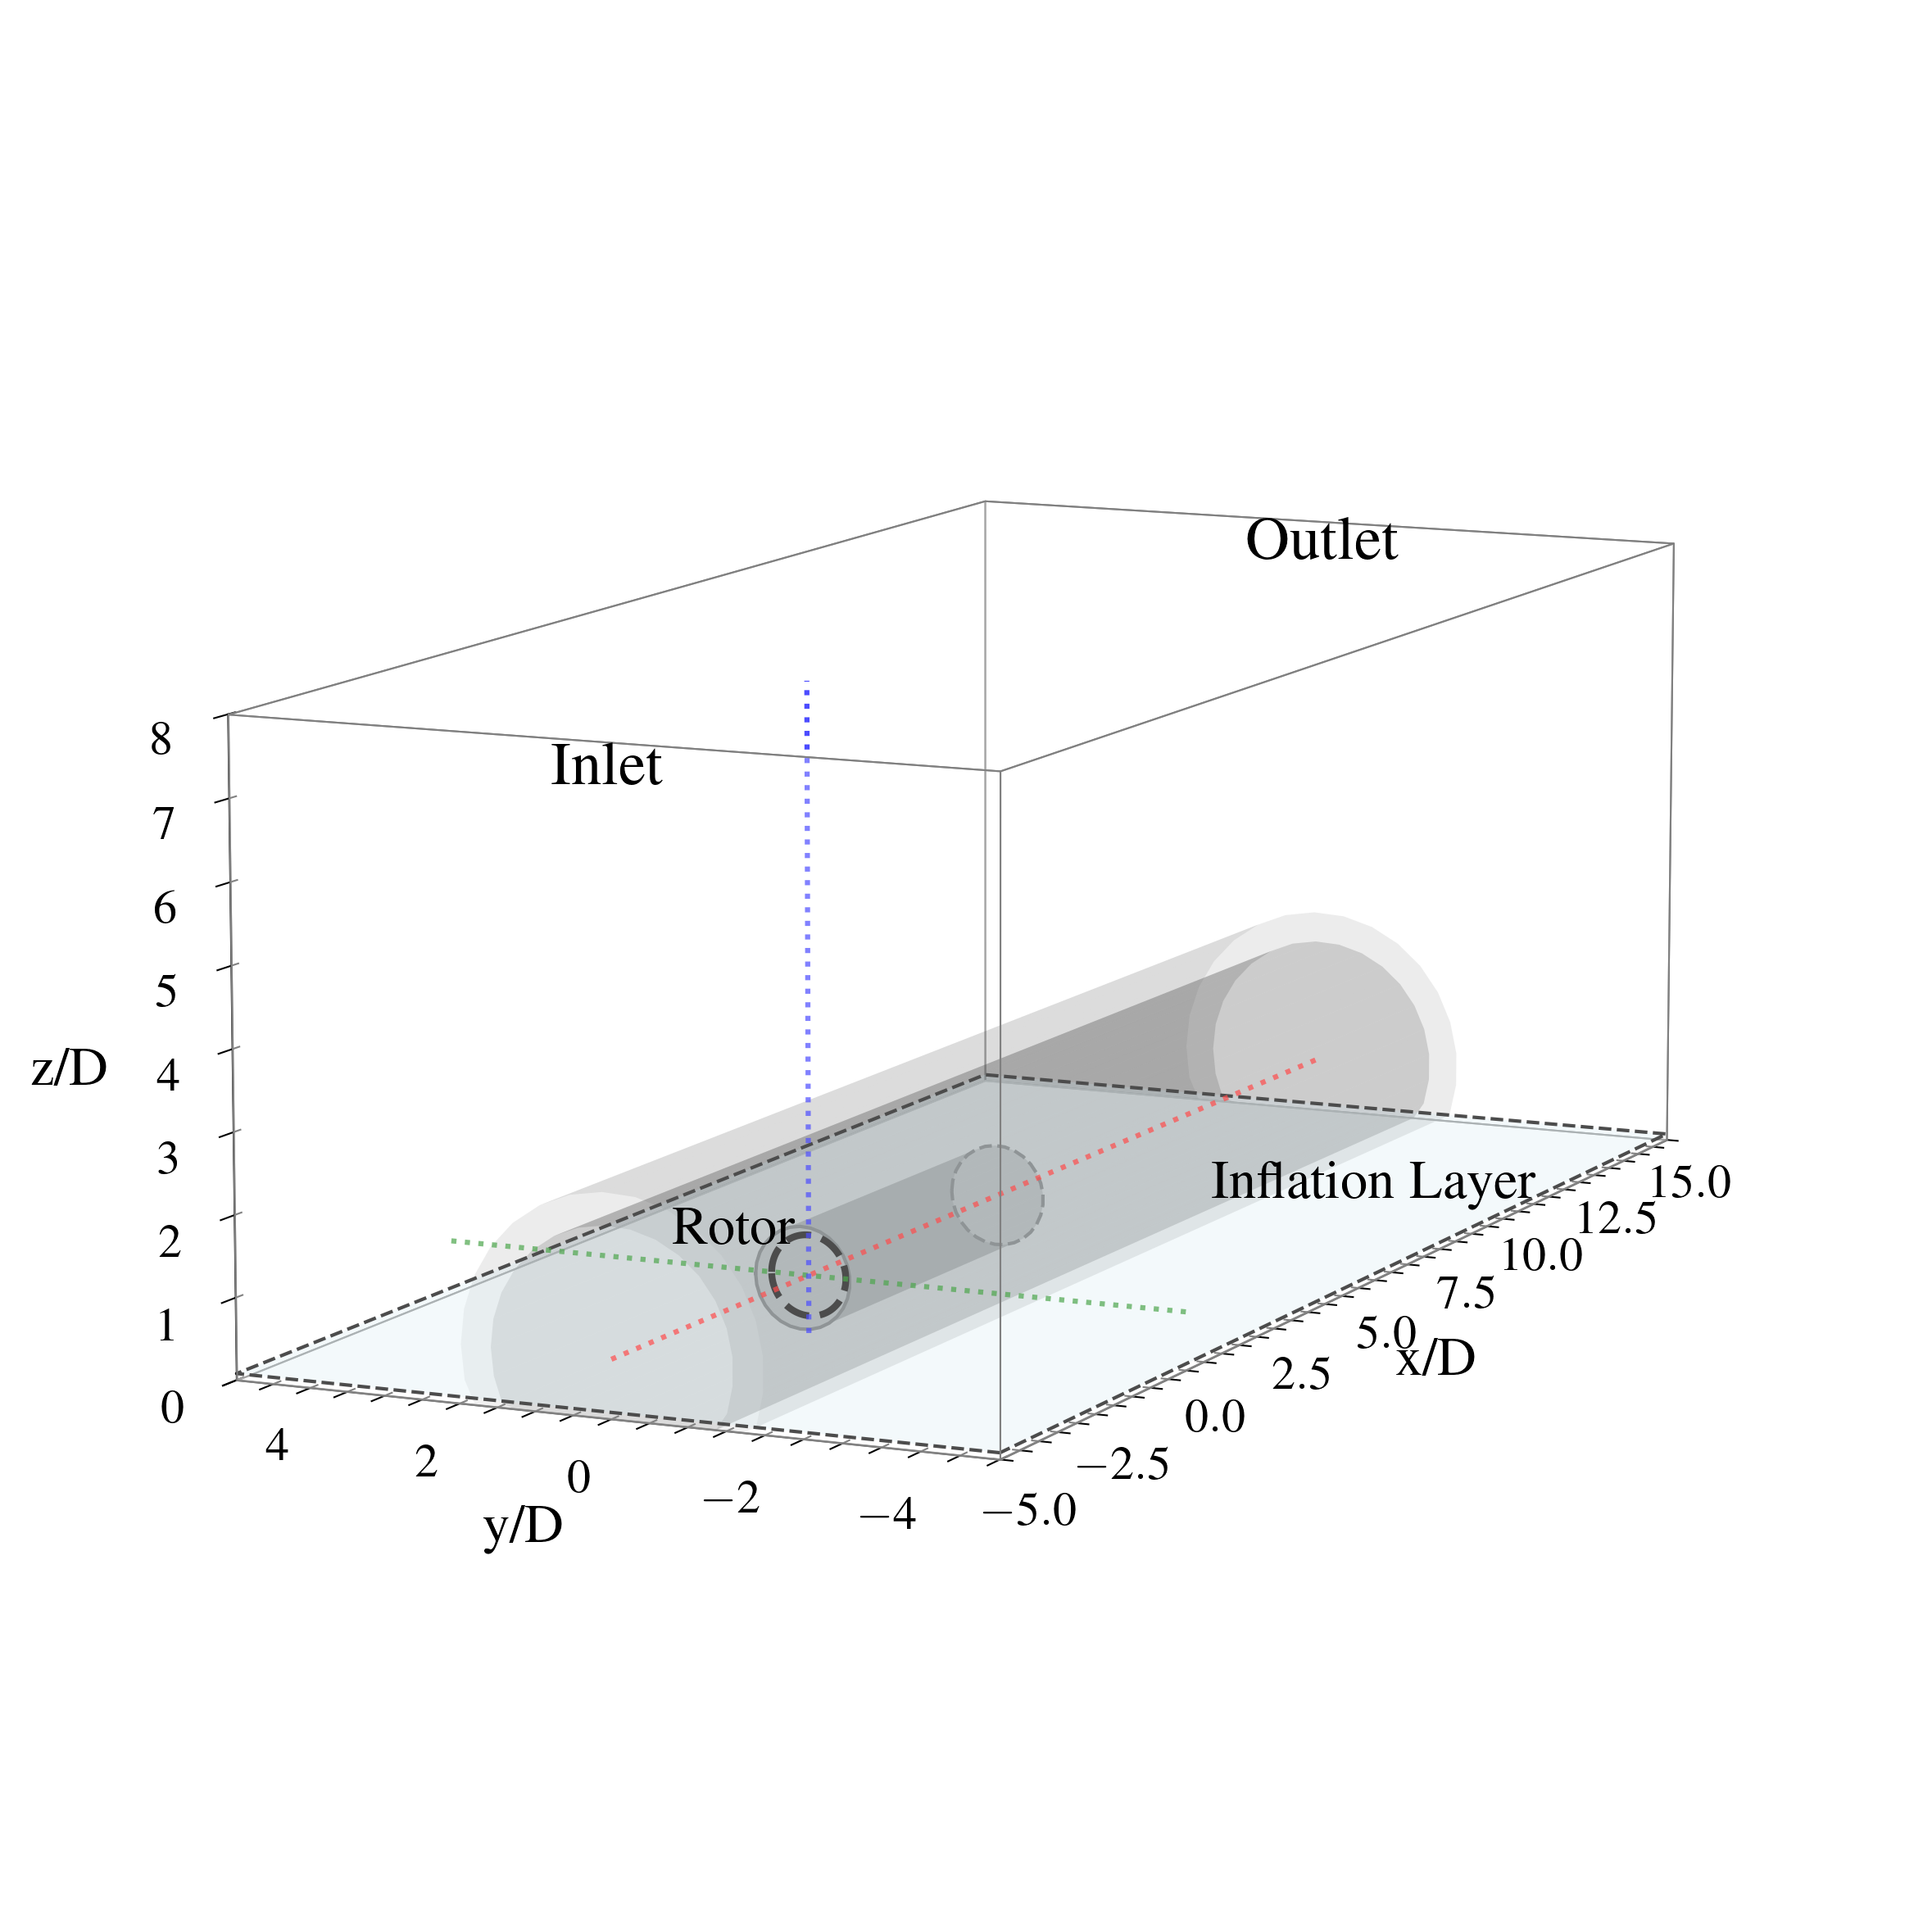
\includegraphics[width=\linewidth, trim= 0 100 0 0,clip]{methodology/img/domain_3d_abl.png}
        \caption{}
    \end{subfigure}
    \hfill
    \begin{subfigure}[b]{0.49\textwidth}
        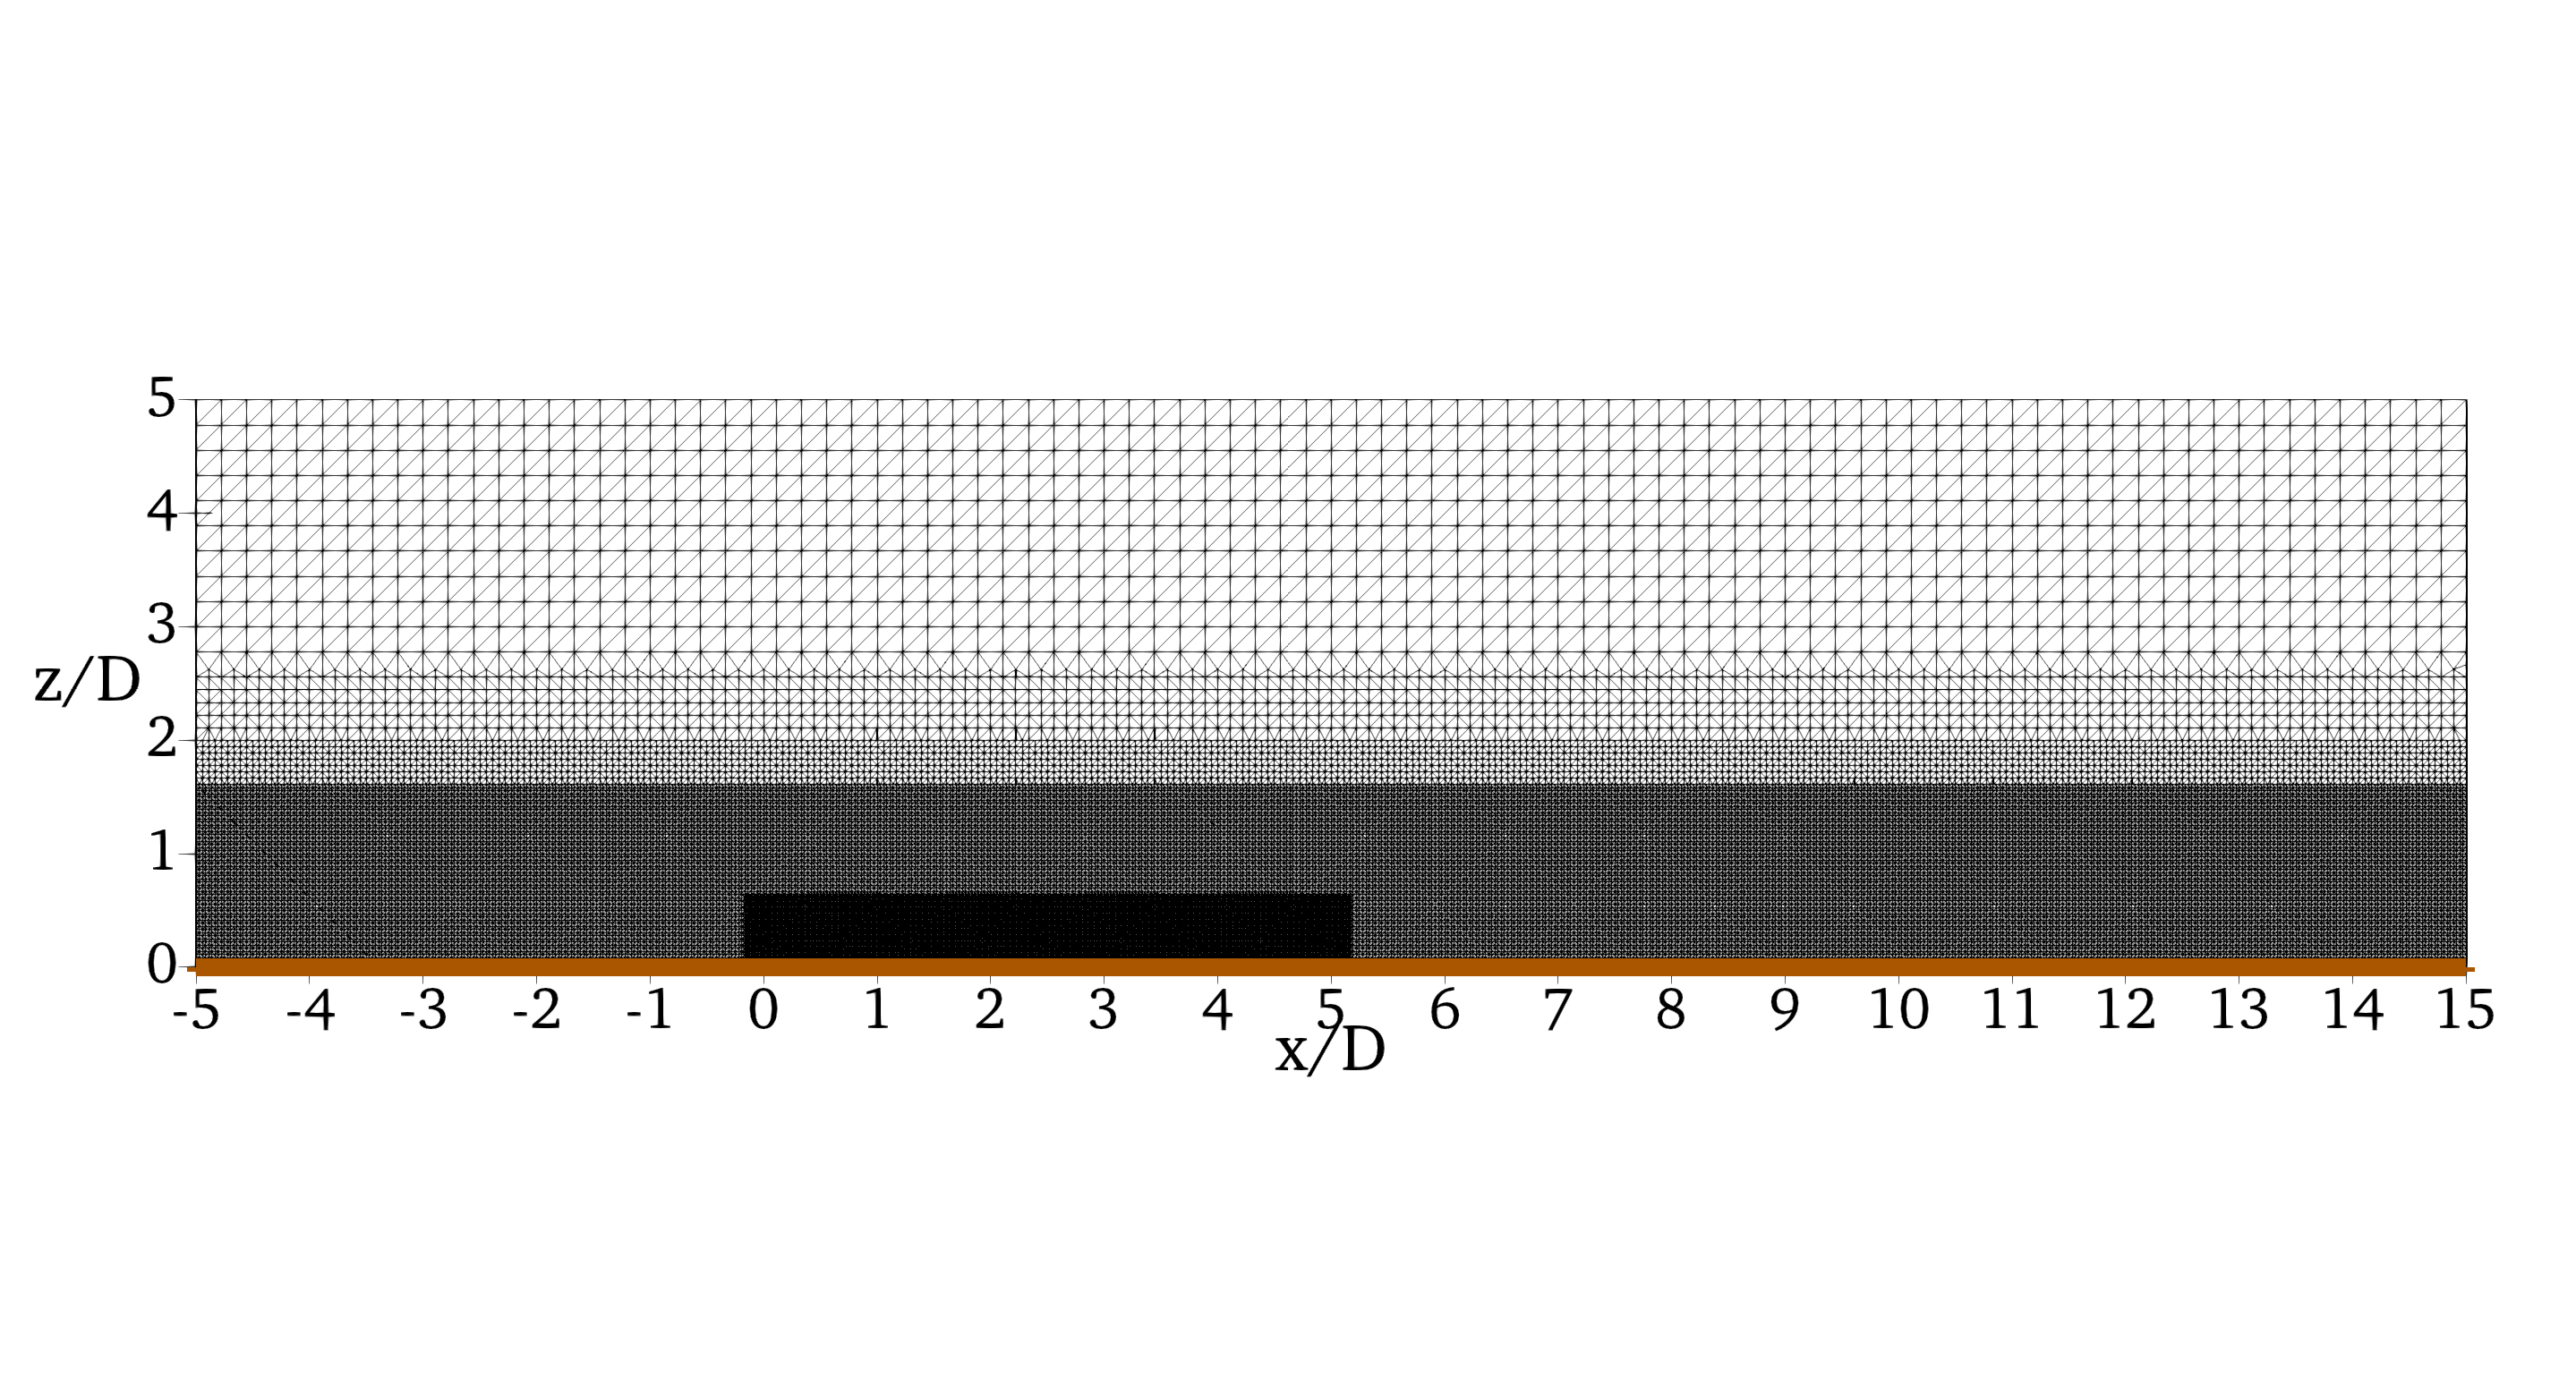
\includegraphics[width=\linewidth]{methodology/img/slice_mesh.png}
        \caption{}
    \end{subfigure}
    \caption{Computational domain (a) and refinement levels represented in (b).}
    \label{fig:mesh}
\end{figure*}

Moreover, the same domain has been used to test the trained models and the mesh refinement influence on the results: while the computational domain and the refinement levels are the same, the minimum and maximum cell size are varied to generate coarser meshes, leading to $\sim15.9$, $\sim9.1$ and $\sim4.2$ million cells with a minimum cell size of $\sim2.25$ m, $\sim2.82$ m and $\sim3.94$ m respectively near the rotor and a $\times 16$ cell size at the domain boundaries.

The CFD simulations were run on a high-performance computing workstation equipped with two AMD EPYC 9534 64-Core processors, for a total of 128 physical cores and 256 threads.

The three types of simulations (RANS, LES and modified RANS) results are shown in Fig.~\ref{fig:cfds}.
\begin{figure*}[h]
    \centering
    \begin{subfigure}[b]{0.32\textwidth}
        \centering
        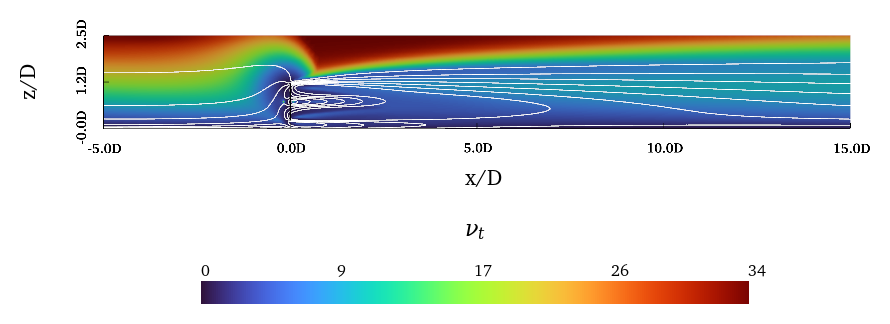
\includegraphics[width=\linewidth]{methodology/img/cfds_rans_nut_xz.png}
        \caption{}
    \end{subfigure}
    \hfill
    \begin{subfigure}[b]{0.32\textwidth}
        \centering
        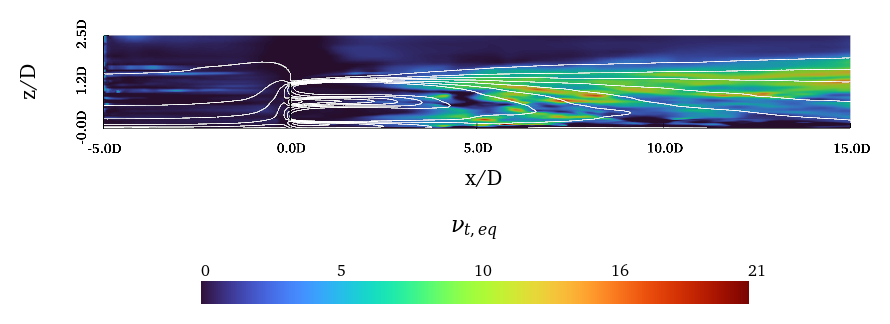
\includegraphics[width=\linewidth]{methodology/img/cfds_les_nutEq_xz.png}
        \caption{}
    \end{subfigure}
    \hfill
    \begin{subfigure}[b]{0.32\textwidth}
        \centering
        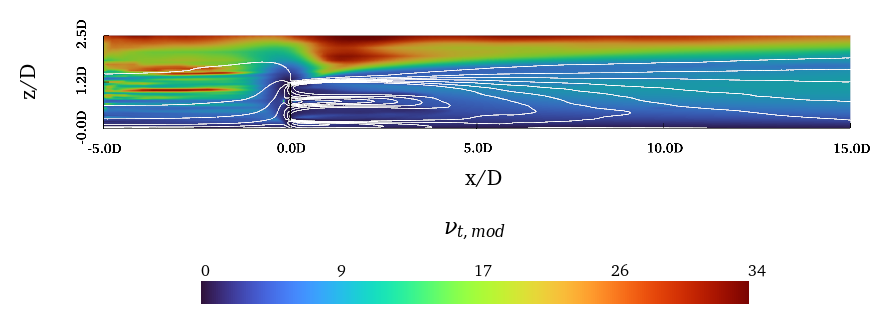
\includegraphics[width=\linewidth]{methodology/img/cfds_modified_nut_xz.png}
        \caption{}
    \end{subfigure}
    \caption{Eddy viscosity fields on the $xz$ plane: (a) original RANS $\nu_t$, (b) LES-equivalent $\nu_{t,eq}$, and (c) modified RANS $\nu_{t,mod}$. The black and white isolines highlight the velocity magnitude contours for RANS simulation and mean velocity ones for the LES and modified RANS simulations.}
    \label{fig:cfds}
\end{figure*}


\subsection{ML methodologies}
\label{sec:ML_part}
Different ML techniques are employed in this study to predict the modified eddy viscosity field $\nu_t$ and the corresponding $\vec{U}$, $p$ and $k$ fields. These methods include both CA and NN, as described in the following.

All the ML models were trained on the same workstation, equipped with an Intel Core i9-10980XE CPU running at 3.00 GHz, with 18 physical cores and 36 threads, and a single NVIDIA Quadro RTX 6000 GPU with 24 GB of dedicated memory.

\subsubsection{Clustering model}
\label{sec:clustering}
This work entails the use of a CA as a cornerstone of all the analysis. This, as in \cite{Carloni2026,Clustering_tieghi}, is done to identify the different flow regions in the wake of the rotor, which are characterised by different dynamics and thus require different modeling approaches.
Moreover, the usage of the CA has an advantage in terms of interpretability of the results and in terms of generalisation capabilities of the trained models: in fact it allows to move from a cell-wise prediction of the $\nu_t$ field to a region-wise prediction, which is more robust and less affected by the mesh refinement and by the geometrical details of the domain.

In fact, clustering algorithms are unsupervised ML techniques that allow to group data points in clusters based on their similarity.
Many different CAs exist in literature and with different characteristics, but in this work the K-means algorithm is used as in \cite{Carloni2026,Clustering_tieghi} for many reasons: it is proven to be effective in identifying the different flow regions in the wake of the rotor and its computational complexity scales well with the size of the dataset, which is a crucial aspect in this study given the large amount of data generated by the CFD simulations. 
The clustering pipeline was implemented in a Python environment leveraging the \textit{scikit-learn} \cite{scikit-learn} open-source library. The K-means algorithm partitions the dataset by minimising the within-cluster sum of squares, the quantity reported by \textit{scikit-learn} as the \textit{inertia} of the clustering and defined as:
\begin{equation}
    \mathrm{Inertia} = \sum_{i=1}^{K} \sum_{x_j \in C_i} \lVert x_j - \mu_i \rVert^2 ,
\end{equation}
where $K$ is the number of clusters, $C_i$ is the set of data points in cluster $i$, $x_j$ is a data point belonging to cluster $i$ and $\mu_i$ is its centroid. The algorithm iteratively assigns each data point to the nearest centroid and updates the centroids until convergence is reached.
To select the optimal number of clusters, the elbow method is used, analysing the inertia as a function of the number of clusters $K$: the chosen $K$ corresponds to the point beyond which additional clusters yield only a marginal reduction of the inertia.
To ensure a correct clustering of the data, the features are previously normalised via a Min-Max normalisation \cite{scikit-learn},
\begin{equation}
    x' = \frac{x - x_{min}}{x_{max} - x_{min}} .
\end{equation}
Then, as done in \cite{Carloni2026,Clustering_tieghi}, the features are projected on a cylindrical reference system centered on the rotor and a subset of them is selected based on the PCA analysis and on the physical understanding of the problem, to ensure a correct clustering of the data both in terms of data analysis and physical interpretation of the results.
Since the exact pipeline has been already described in previous works \cite{Carloni2026,Clustering_tieghi}, here only the main results are presented (i.e., the optimal number of clusters  and clustering features).
Results of the clustering methodology are reported in Sec.~\ref{sec:clustering_results}.

A brief review of the clustering pipeline together with the CFD one is reported in Fig.~\ref{fig:methodology_pipeline}.
\begin{figure*}[h]
    \centering
    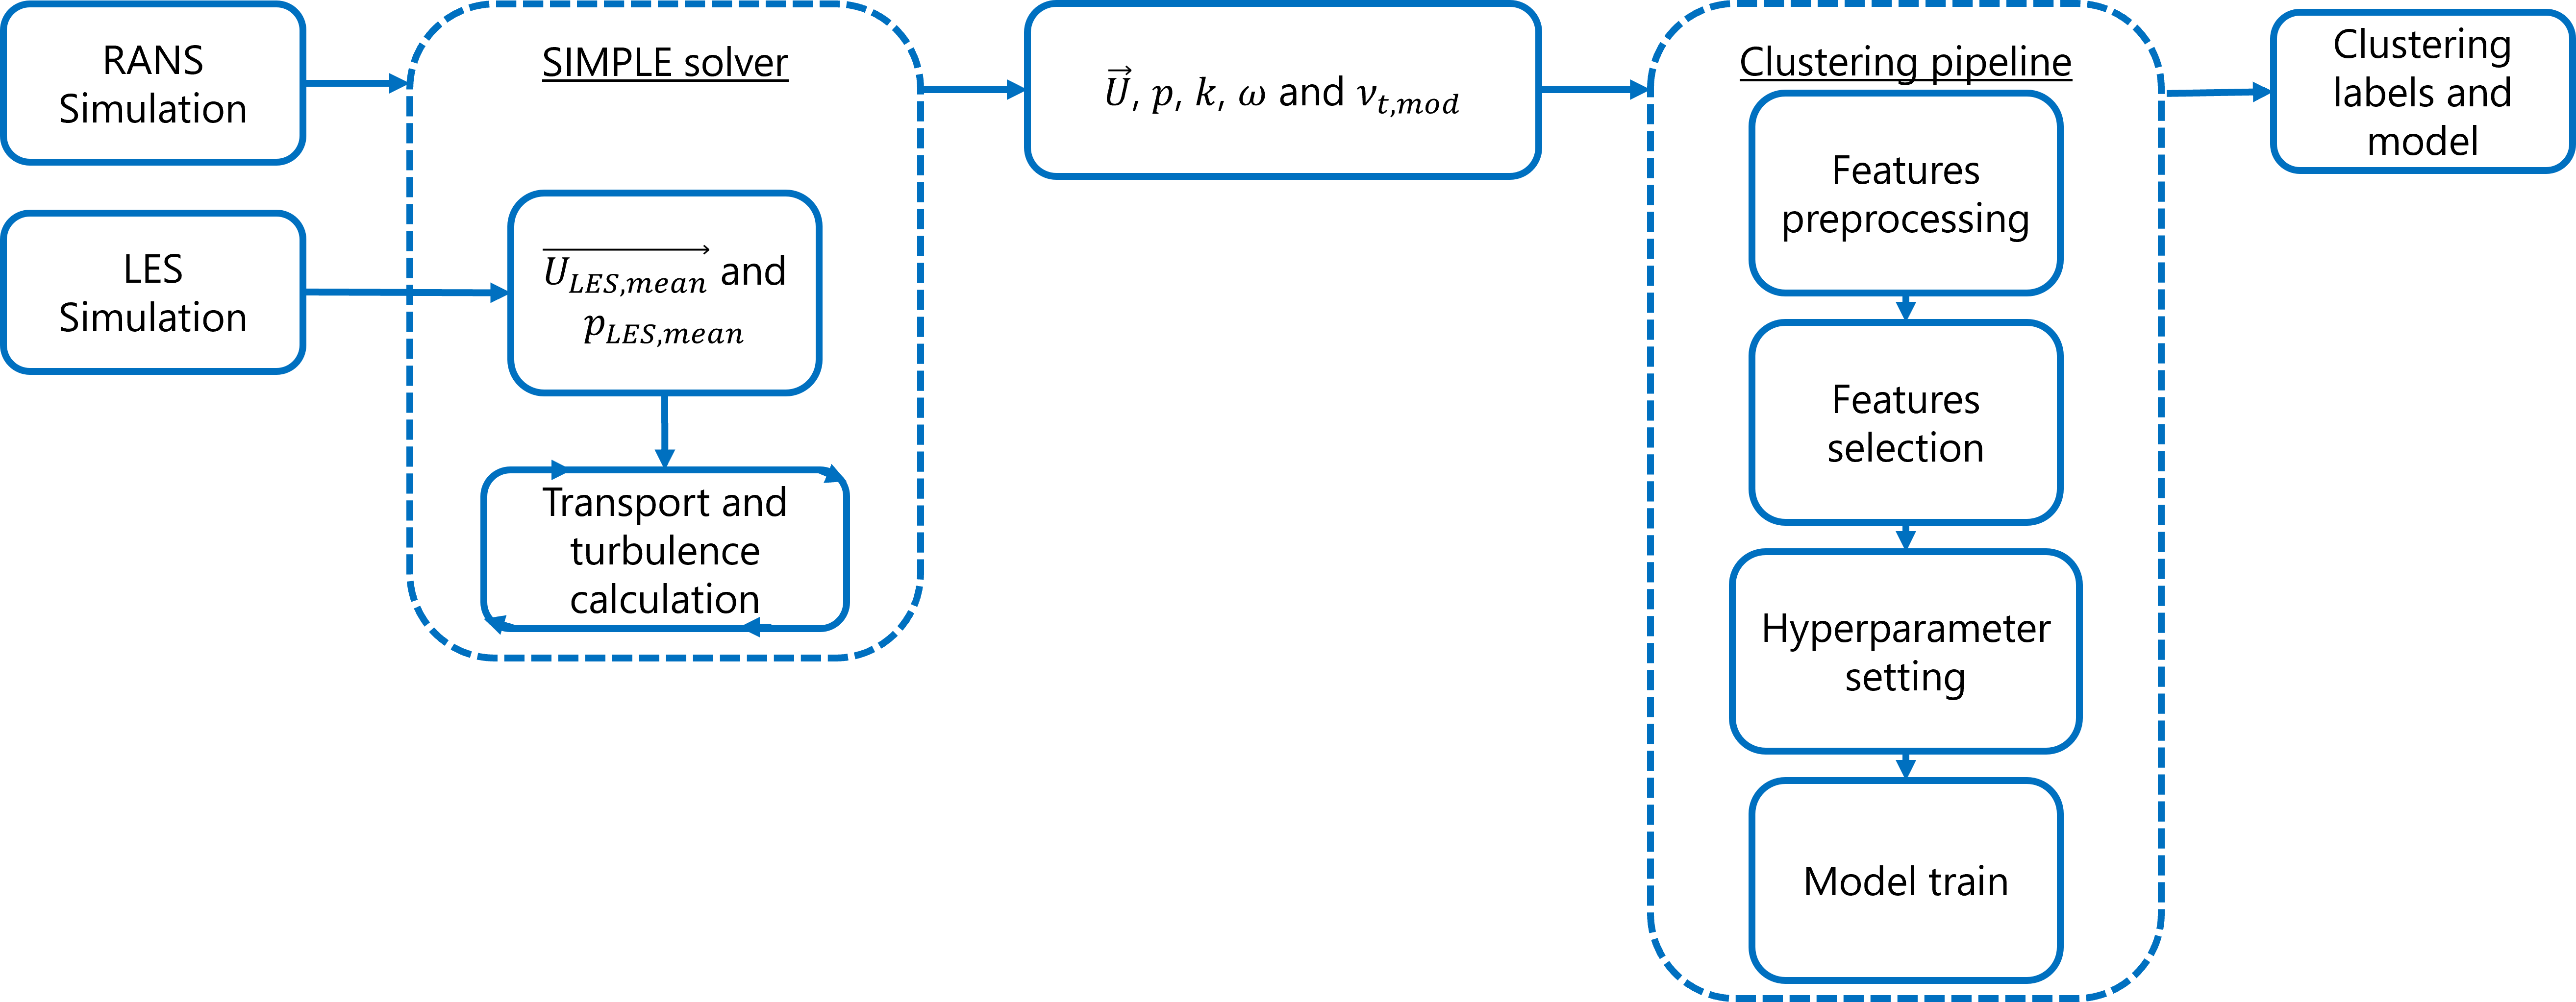
\includegraphics[width=1\textwidth]{methodology/img/clustering_pipelinepng.png}
    \caption{CFD and ML pipeline.}
    \label{fig:methodology_pipeline}
\end{figure*}

\subsubsection{NN model}
\label{sec:NN}
Finally, after the clustering of the data, a NN is trained to predict the $\nu_{t,ML}$ field.
In this work, $\nu_t$ denotes the kinematic turbulent viscosity, namely the scalar field used in the Boussinesq approximation to model the effect of the unresolved turbulent stresses on the mean momentum equation. It enters the RANS equations through the effective viscosity,
\begin{equation}
    \nu_{eff} = \nu + \nu_t ,
\end{equation}
where $\nu$ is the molecular kinematic viscosity of the fluid. The reference quantity used to define the regression target is the correction between the baseline RANS eddy viscosity $\nu_{t,\mathrm{RANS}}$ and an equivalent LES eddy viscosity $\nu_{t,eq}$.

The field $\nu_{t,eq}$ is obtained by projecting the deviatoric part of the LES turbulent stress tensor onto the Boussinesq form. The total deviatoric turbulent stress is written as the sum of the resolved and subgrid-scale contributions,
\begin{equation}
    \Sigma_{ij}^{dev} =
    \left(R_{ij}^{res}\right)^{dev} + \tau_{ij}^{sgs,dev}
    \simeq -2 \nu_{t,eq} S_{ij},
\end{equation}
where $S_{ij}$ is the resolved strain-rate tensor and $R_{ij}^{res}$ is the resolved stress tensor. Assuming a Smagorinsky-type subgrid contribution,
\begin{equation}
    \tau_{ij}^{sgs,dev} = -2 \nu_{sgs} S_{ij},
\end{equation}
$\nu_{t,eq}$ is evaluated as the scalar viscosity that minimises the Frobenius norm
\begin{equation}
    J(\nu_t) =
    \left[
    \left(R_{ij}^{res}\right)^{dev}
    -2\nu_{sgs}S_{ij}
    +2\nu_t S_{ij}
    \right]
    :
    \left[
    \left(R_{ij}^{res}\right)^{dev}
    -2\nu_{sgs}S_{ij}
    +2\nu_t S_{ij}
    \right].
\end{equation}
The optimality condition $\partial J/\partial \nu_t=0$ gives
\begin{equation}
    \nu_{t,eq}
    =
    \nu_{sgs}
    -
    \frac{\left(R_{ij}^{res}\right)^{dev}S_{ij}}
    {2S_{ij}S_{ij}} .
\end{equation}
By construction, $\nu_{t,eq}$ is the scalar eddy viscosity that best reproduces, in a least-squares sense, the deviatoric LES turbulent stress within the Boussinesq framework. It therefore does not encode the full Reynolds-stress anisotropy; this is a deliberate choice, consistent with the scalar closure targeted here and with the requirement that the resulting field be directly usable by a standard eddy-viscosity solver, where the goal is to reproduce the LES turbulent mixing rather than its tensorial structure.

Rather than predicting $\nu_{t,eq}$ directly, the NN is trained to predict the discrepancy between the RANS eddy viscosity and the LES-equivalent eddy viscosity,
\begin{equation}
    \Delta \nu_t = \nu_{t,eq} - \nu_{t,\mathrm{RANS}}.
\end{equation}
The final data-driven eddy viscosity is therefore reconstructed as
\begin{equation}
    \nu_{t,ML} = \nu_{t,\mathrm{RANS}} + \Delta \nu_{t,ML}.
\end{equation}
This formulation allows the network to learn the correction required to move from the baseline RANS eddy viscosity to the LES-equivalent eddy viscosity used as target closure.

The regression model is a Multi-Layer Perceptron (MLP), implemented in TensorFlow-Keras \cite{tensorflow2015-whitepaper}, with a single scalar output corresponding to $\Delta \nu_{t,ML}$. The input vector is defined at cell level and includes $\vec{U}_{cyl}$, $k$, $\nu_{t,\mathrm{RANS}}$, the distance from the assigned cluster centroid in the normalised clustering space, the non-dimensional vertical and axial coordinates $z/D$ and $x/D$, and the cluster labels. The continuous features are standardised using a Standard Scaler, while the cluster labels are encoded through one-hot encoding. The target $\Delta \nu_t$ is also standardised before training.

Prior to the split, cells in the far-upstream inflow region ($x/D < -2.5$) are excluded from the training and validation sets, as the NN performance in that zone is inherently limited by the synthetic inlet boundary condition; this reduces the dataset from $\sim 180k$ cells to $\sim 160k$ cells retained for training and validation. The remaining points are split into training and validation subsets using an 80/20 split, stratified with respect to the cluster labels in order to preserve the same distribution of flow regions in both sets. During training, sample weights are introduced to compensate for cluster imbalance through inverse-frequency weighting. An additional axial weight is applied to increase the relevance of downstream wake samples, according to
\begin{equation}
    w_{ax} = 1 + \max(x/D,0),
\end{equation}
and the final sample weight is obtained as the product of the cluster and axial weights.

The MLP architecture is composed of a sequence of fully connected residual blocks. Each block contains a Dense layer with L2 kernel regularization, Layer Normalization, a GELU activation function and Dropout. When residual connections are enabled, the block input is added to the block output; if the two tensors have different dimensions, the shortcut is first projected through a linear Dense layer. The hidden-layer widths are progressively reduced according to
\begin{equation}
    n_i = \max \left( \mathrm{round}(n_0 r^{i-1}), 32 \right),
\end{equation}
where $n_0$ is the initial number of neurons and $r$ is a width-decay factor. This is done in order to reduce the complexity of the model and prevent overfitting and also to catch more complex relationships between the input features in the first layers and to produce a more compact representation. The output layer is a linear Dense layer with one neuron. The model is trained by minimising a weighted Huber loss using the Adam optimizer, while the mean absolute error is monitored as an additional metric.

The architecture and training hyperparameters are fixed through a manual preset, selected from preliminary tests and kept unchanged for the reported training. The adopted configuration is reported in Tab.~\ref{tab:nn_manual_configuration}.

\begin{table}[h]
    \centering
    \caption{Manual configuration adopted for the MLP training.}
    \label{tab:nn_manual_configuration}
    \begin{tabular}{lc}
        \hline
        Hyperparameter & Value \\
        \hline
        Hidden blocks & 7 \\
        Initial neurons $n_0$ & 192 \\
        Width decay $r$ & 0.78 \\
        Hidden-layer widths & 192, 150, 117, 91, 71, 55, 43 \\
        Activation function & GELU \\
        Layer Normalization & True \\
        Residual connections & True \\
        Dropout rate & 0.05 \\
        L2 regularization & $1\cdot10^{-4}$ \\
        Learning rate & $1.5\cdot10^{-4}$ \\
        Huber $\delta$ & 1.0 \\
        Batch size & 128 \\
        \hline
    \end{tabular}
\end{table}

The final model is trained with early stopping on the validation loss and a learning-rate reduction on plateau. The maximum number of epochs is controlled by the training configuration and was set to 400 in the reported run. In addition to the training and validation loss, the RMSE and physical-space validation metrics are monitored during training.

Results of the NN training and testing are reported in Sec.~\ref{sec:NN_results} as for the clustering ones.
MLP training pipeline is summarised in Fig.~\ref{fig:mlp_pipeline}.
\begin{figure*}[h]
    \centering
    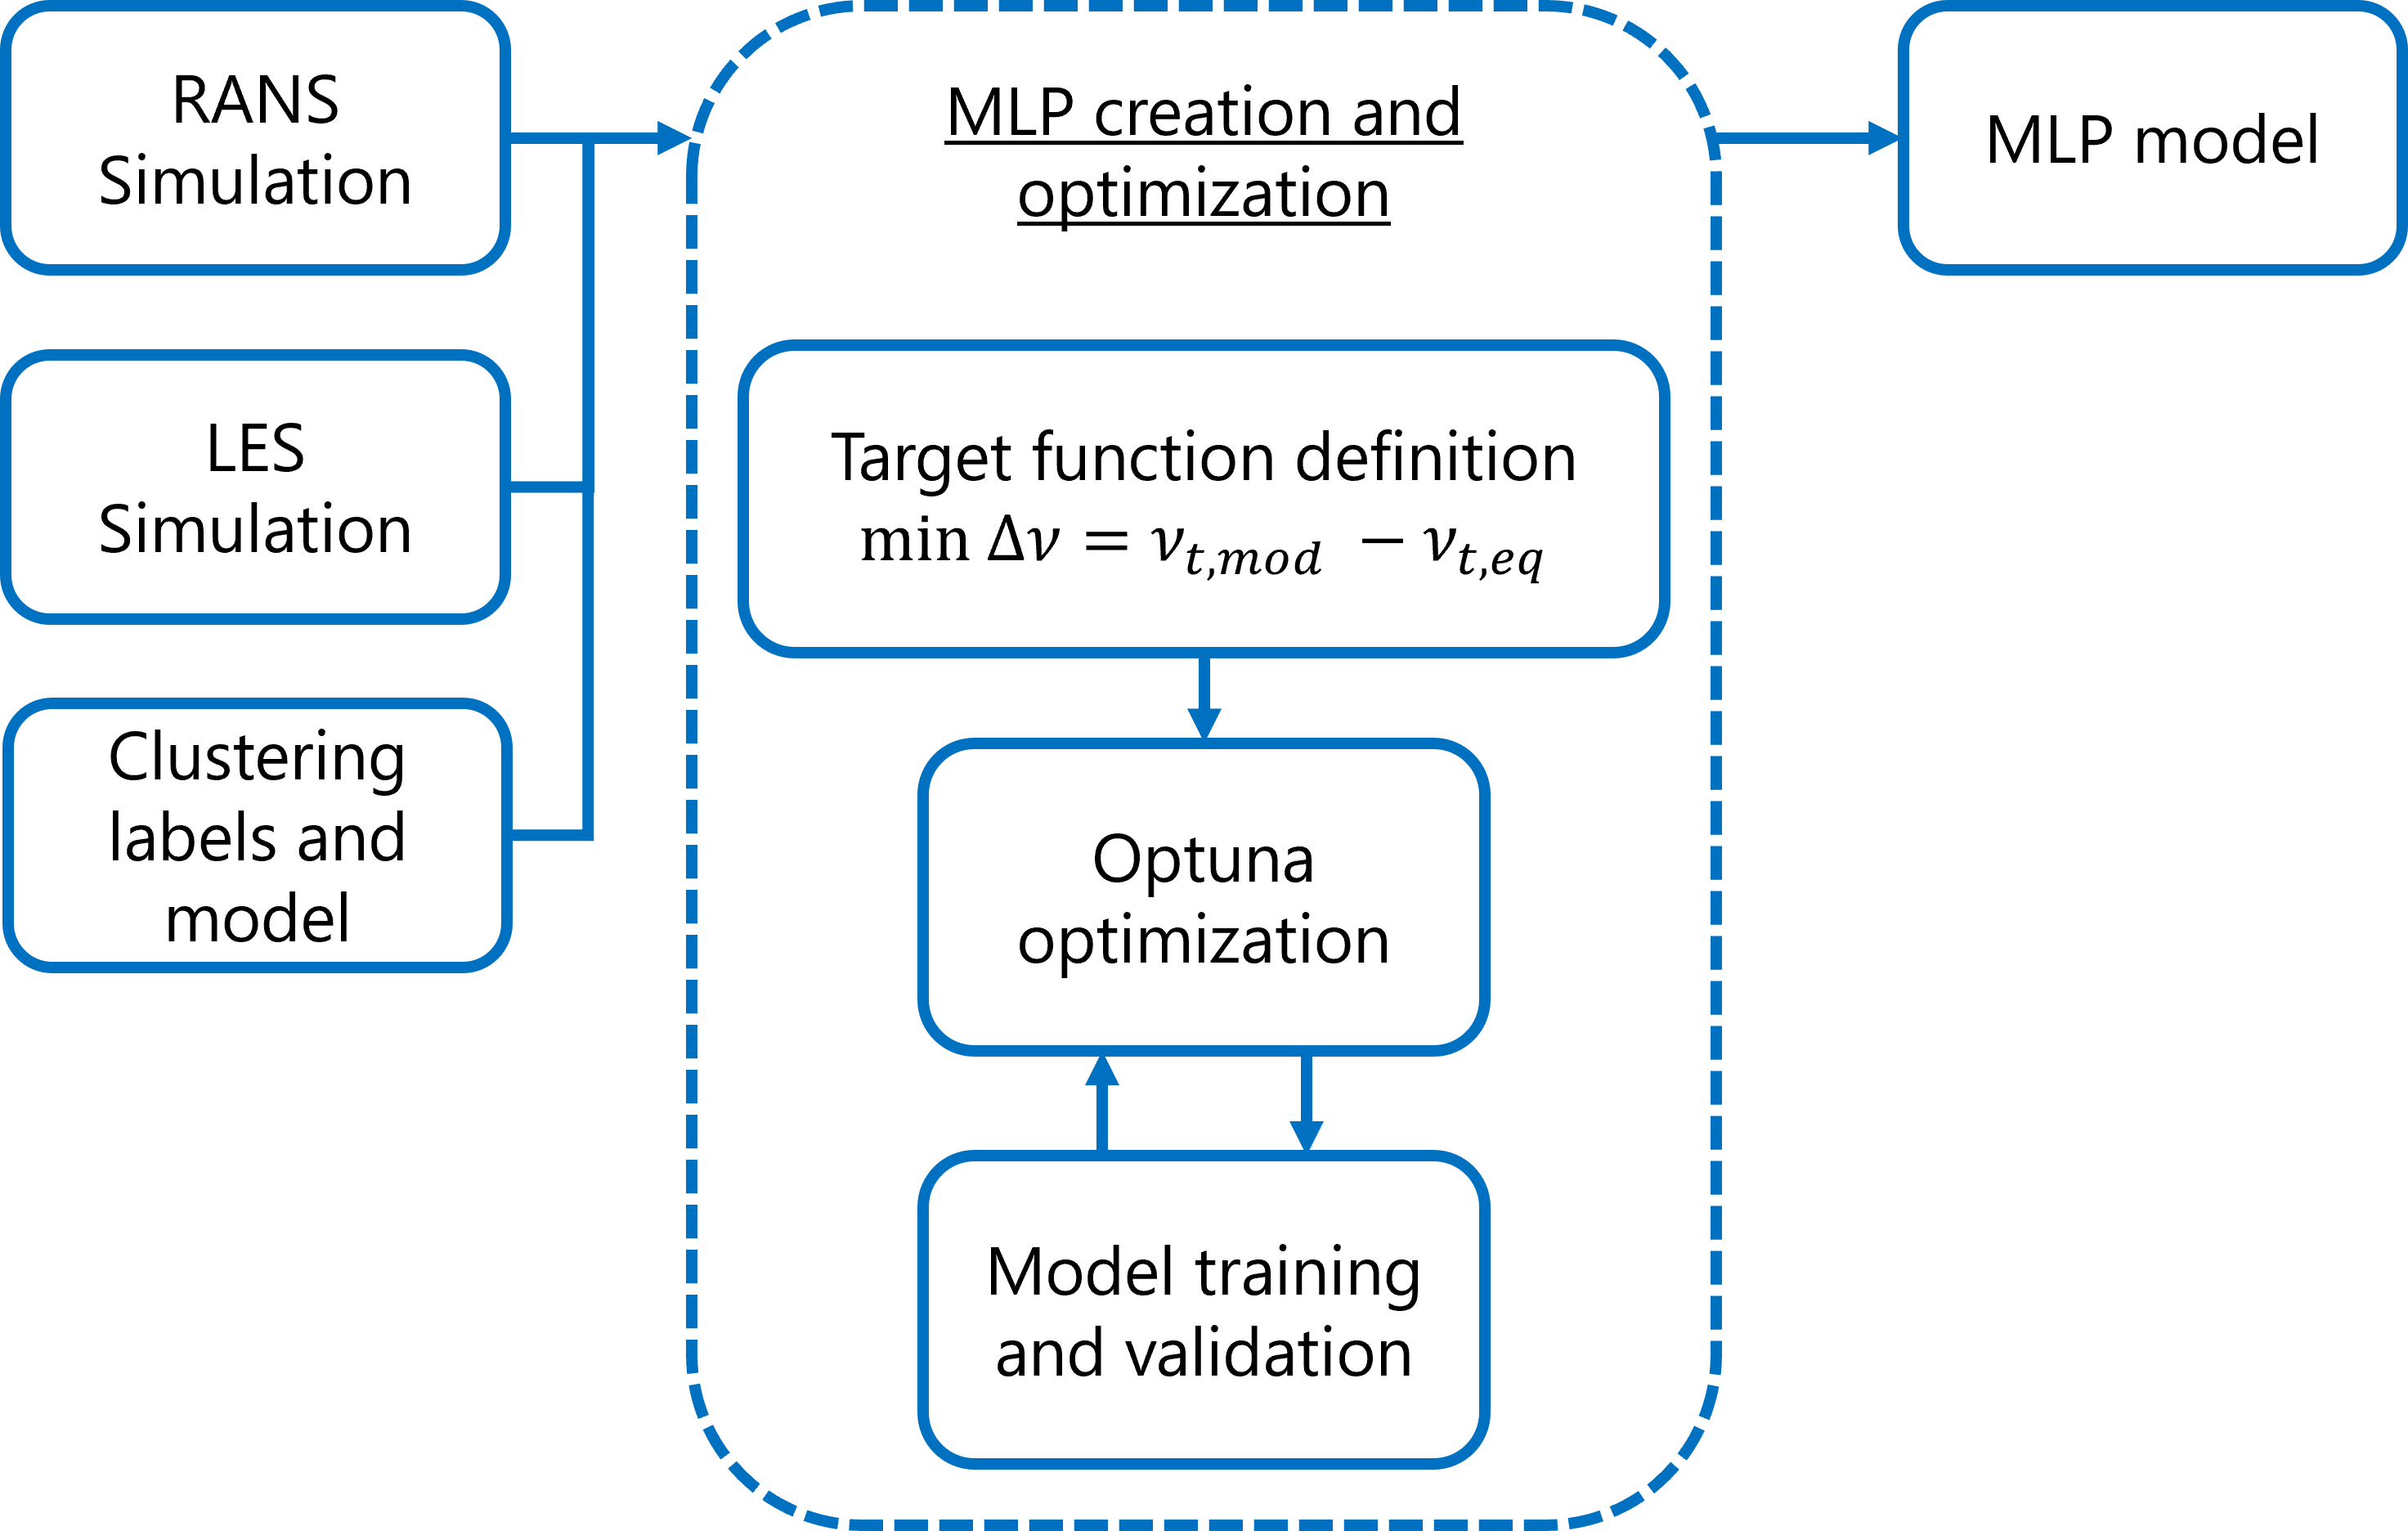
\includegraphics[width=0.6\textwidth]{methodology/img/NNpipeline.png}
    \caption{MLP training pipeline.}
    \label{fig:mlp_pipeline}
\end{figure*}

\subsection{ML-based RANS model implementation}
\label{sec:ml_pimple_pipeline}
Finally all the trained models are implemented in the RANS solver of OpenFOAM to test their performance in a predictive setting. To do so, a modified version of the PIMPLE algorithm is implemented as in Fig.~\ref{fig:pimple_pipeline}.
\begin{figure*}
    \centering
    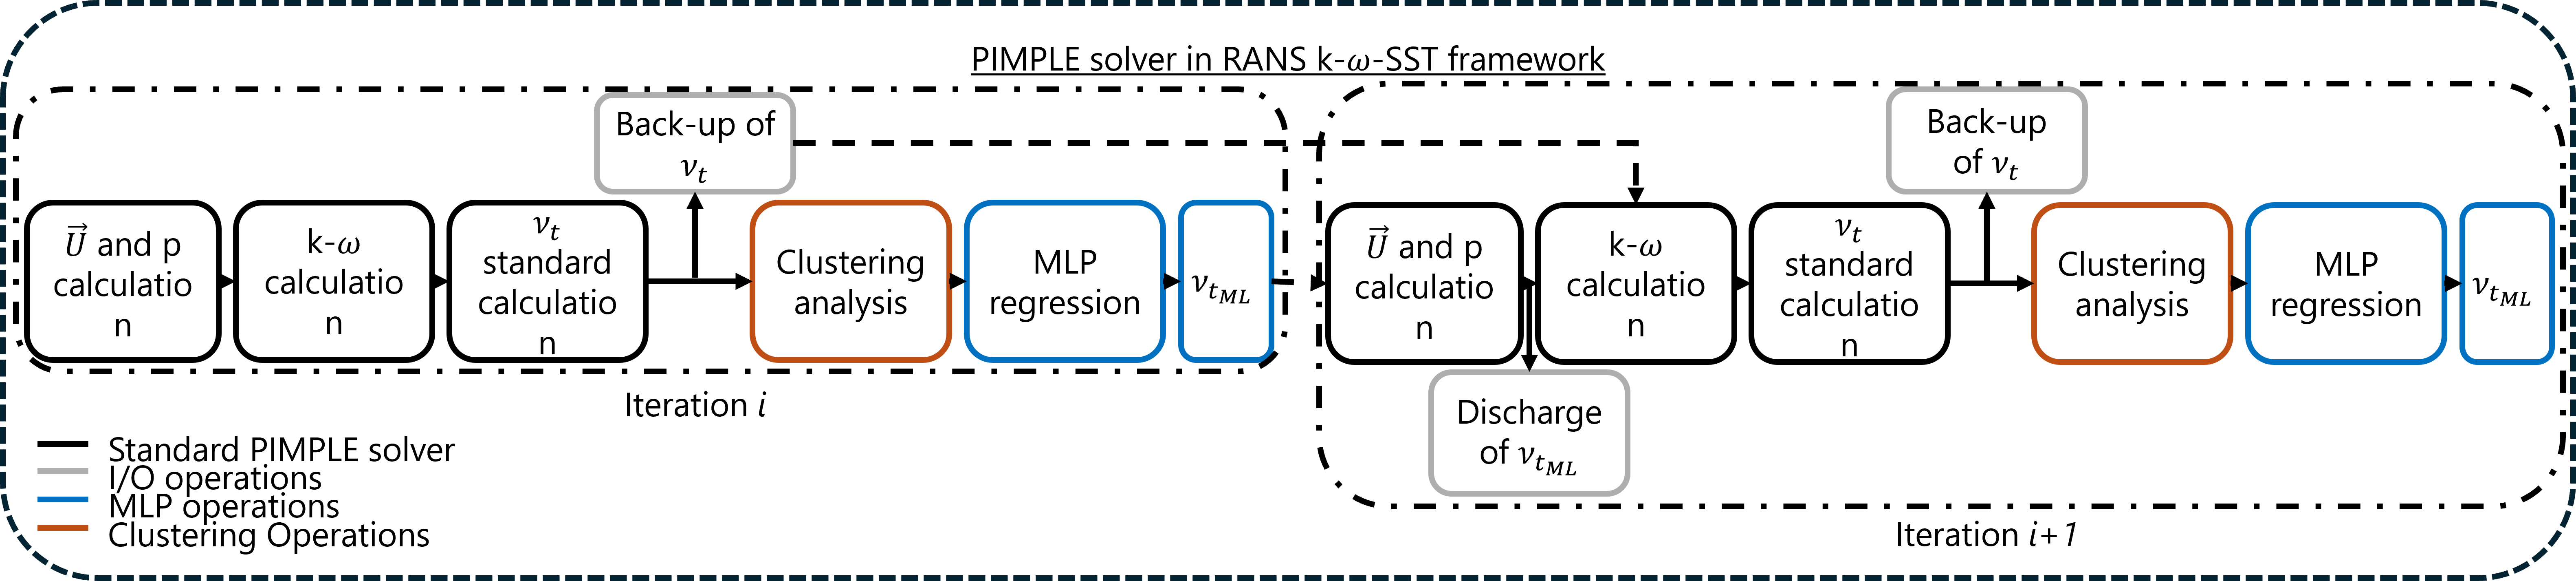
\includegraphics[width=1\textwidth]{methodology/img/solver_pipeline.png}
    \caption{ML-based PIMPLE algorithm.}
    \label{fig:pimple_pipeline}
\end{figure*}
The $\vec{U}_{cyl}$-$p$ PIMPLE internal loop is not modified, while the turbulence correction loop is: the first iteration of the solver is executed with the standard $k$-$\omega$ SST model to compute the $\vec{U}$, $p$, $k$, $\omega$ and $\nu_t$ fields, then the clustering model is applied to assign a cluster label to each cell and the NN is applied to predict the $\nu_{t,ML}$ field; this is then used, in the second iteration of the solver, to compute the $\vec{U}$ and $p$ fields, while the $k$ and $\omega$ fields are still computed with the standard SST model stored in the first iteration and then corrected again with the NN; the same procedure is repeated for the following iterations of the solver.

By design, only the eddy viscosity entering the momentum equations is replaced by the data-driven field, whereas the $k$ and $\omega$ transport equations retain the standard SST formulation and its boundedness treatment. This keeps the correction confined to the closure term and preserves the numerical robustness of the baseline solver: across all the grids and inflow velocities tested, the modified solver reached a stable statistically-steady state without any ad hoc relaxation or limiter on the predicted field. It is also worth stressing that the clustering and NN inference are the only components added to the solver loop, so that the data-driven model is fully embedded in the CFD solver and used predictively, with no LES information supplied at run time.

%%%case study
\section{Case study}
\label{sec:case_study}
To test the proposed methodology, this study considers the NREL-5MW \cite{NREL_5MW} Horizontal-Axis Wind Turbine (HAWT). As cited before, the rotor is modeled with the ALM to reduce the computational cost of the simulations. Number of nodes are changed according to the mesh refinement, to ensure always that $\epsilon \le 2\Delta x$ and $\frac{\Delta b}{\Delta x} \le 0.75$ \cite{inproceedings}. Selected combinations of $\Delta b$ are reported in Tab.~\ref{tab:ALM_parameters} as a function of the mesh refinement.
\begin{table}[h]
    \centering
    \begin{tabular}{c|c|c}
        \textbf{Mesh $\Delta x$ [m]} & $\Delta b$ [m] & $\frac{\Delta b}{\Delta x}$ \\
        \hline
        $\sim 3.94$ & 32 & $\sim0.5$ \\
        $\sim 2.82$ & 44 & $\sim0.5$ \\    
        $\sim 2.25$ & 56 & $\sim0.5$ \\
        $\sim 1.78$ & 71 & $\sim0.5$ \\
    \end{tabular}
    \caption{ALM parameters for the different mesh refinements.}
    \label{tab:ALM_parameters}
\end{table}
An inflow velocity $U_{ref}$ at hub height (i.e., $90$~m from the ground) of $11\,\mathrm{m/s}$ is taken as the single reference condition on which the closure is trained, while two additional inflow velocities of $8$ and $15\,\mathrm{m/s}$ are simulated solely to test the trained model on operating conditions never seen during training. Consistently with the design premise of the methodology, no data from these two conditions, nor from the coarser grids used for testing, enter the training set at any stage: together they constitute a strict out-of-sample assessment of the learned closure. For each condition the ABL logarithmic profile is evaluated from the corresponding hub-height velocity as reported in Eq.~\ref{eq:ABL_log_equation}:
\begin{equation}
    U(z) = U_{ref} \frac{\ln(\frac{z+z_0}{z_0})}{\ln(\frac{z_{ref}+z_0}{z_0})}
    \label{eq:ABL_log_equation}
\end{equation}

The data generated with the CFD campaign was evaluated against literature results \cite{alessio5-mw, Troldborg} as also done in previous studies (e.g., \cite{Carloni2026}). Hence, the results are not reported here for brevity, but the interested reader can refer to the cited works for a detailed validation of the CFD dataset.
Such dataset is then used to extract the training data for the ML models and to test them.
The training dataset is generated by sampling the CFD fields, on the finest grid of the reference $11\,\mathrm{m/s}$ case only, along two planes crossing the rotor centre: one parallel and one perpendicular to the terrain, so as to capture the wake-ABL interaction in both directions. This results in a total of $\sim 180k$ cells for the training dataset, as anticipated in Sec.~\ref{sec:NN}. Deliberately limiting the training data to a single grid and a single operating point keeps the high-fidelity cost to the minimum, and turns every coarser grid and every other inflow velocity into an independent test of the closure rather than an additional training case.
%%%results
\section{Results}
\label{sec:results}
The results are organised as follows. The clustering and neural-network metrics refer to the finest grid, which is the one used for training, whereas the embedded ML-based RANS model is evaluated on the coarser grids, which are never used during training. This separation is intentional: it allows the embedded closure to be assessed strictly out of sample and shows that its benefit over the standard RANS model is twofold, in accuracy and in computational cost.

\subsection{Clustering results}
\label{sec:clustering_results}
First of all the PCA results are shown in Fig.~\ref{fig:pca}. 
\begin{figure}[h]
    \centering
    \begin{subfigure}{0.49\textwidth}
        \centering
        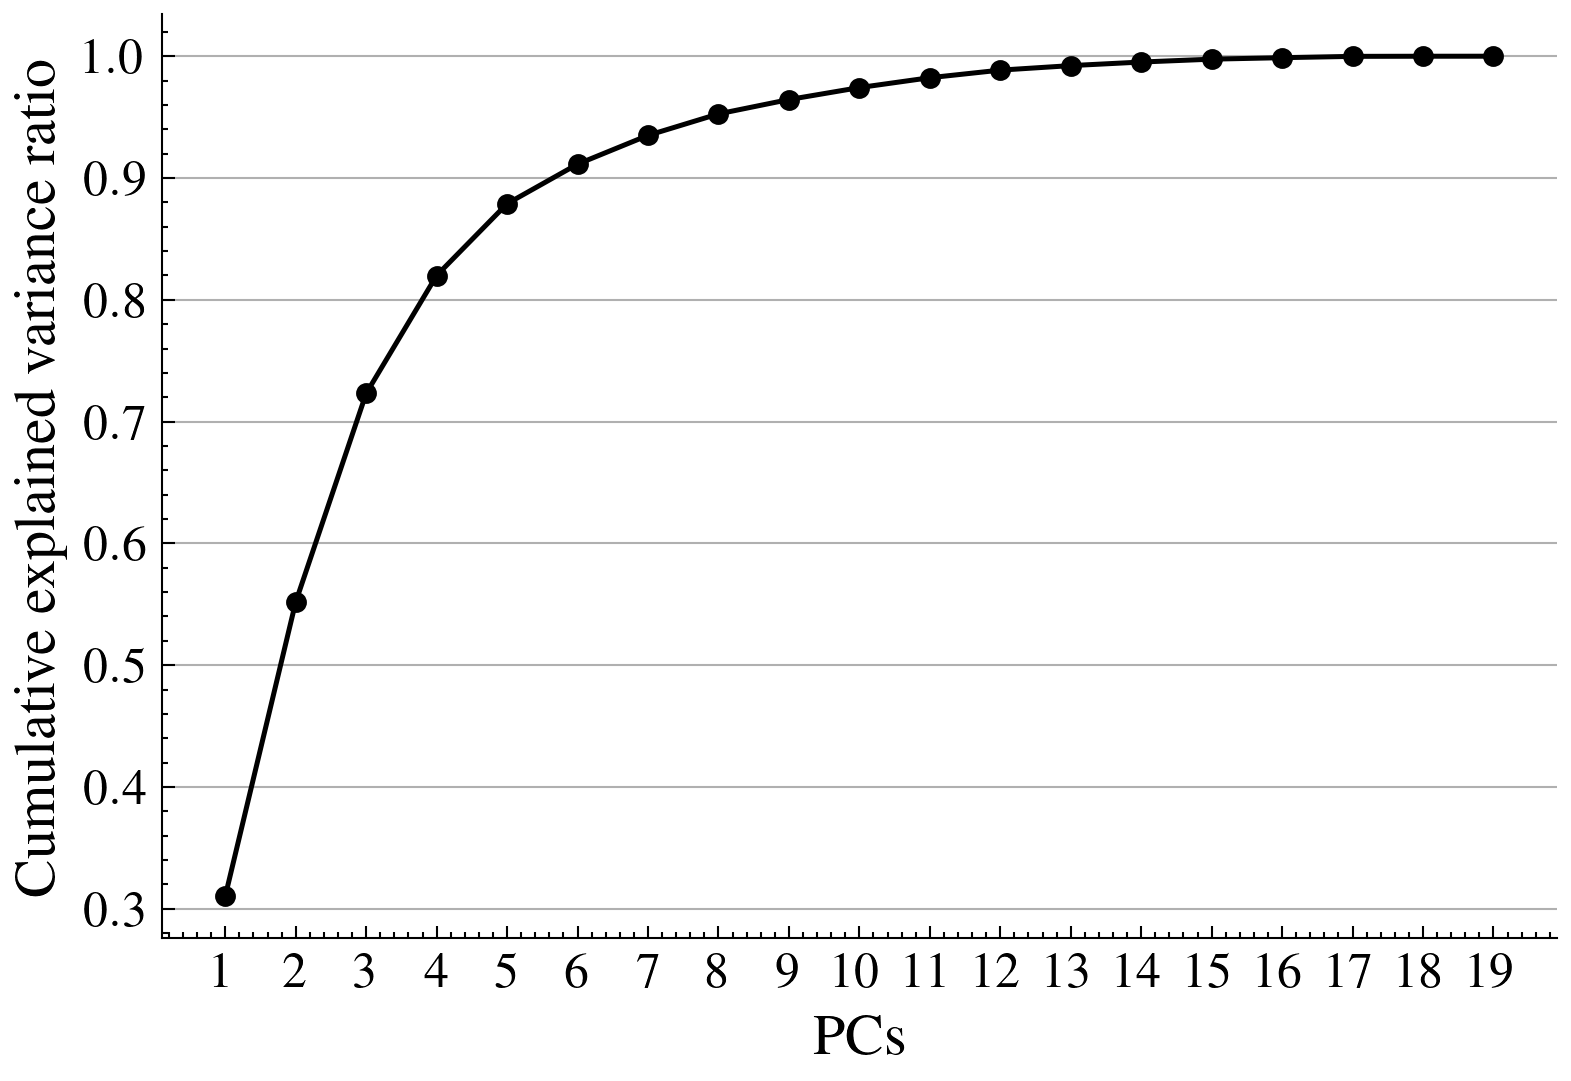
\includegraphics[width=\textwidth]{results/img/pca_explained_variance_ratio.png}
        \caption{}
        \label{fig:pca}
    \end{subfigure}
    \begin{subfigure}{0.49\textwidth}
        \centering
        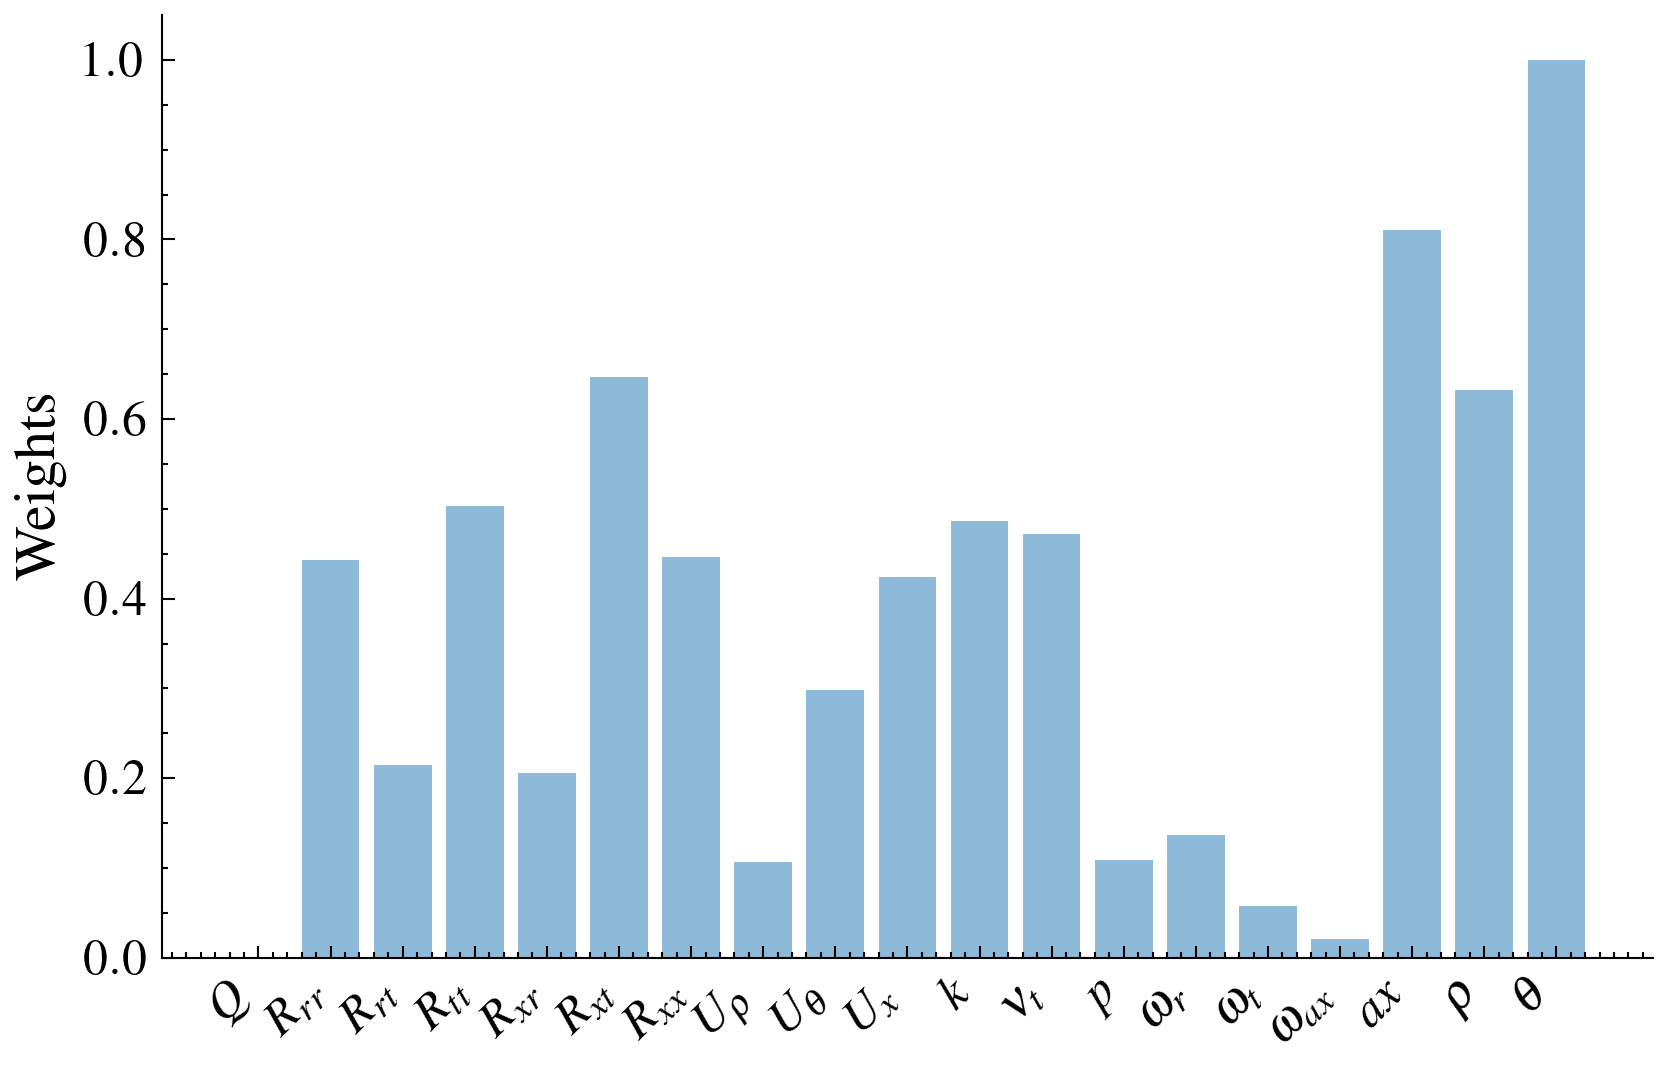
\includegraphics[width=\textwidth]{results/img/pca_features_weights.png}
        \caption{}
        \label{fig:pca_features_weights}
    \end{subfigure}
    \caption{PCA results: (a) explained variance ratio, (b) features weights on the first 6 PCA components.}
\end{figure}
From Fig.~\ref{fig:pca} it can be seen that the first 6 PCs explain more than 90\% of the variance. From Fig.~\ref{fig:pca_features_weights} the influence of the features on the first 6 PCs can be seen. It can be noted that the most influential features are the ones related to the cells coordinates (expressed in cylindrical coordinates) followed by $k$, $\nu_t$ and $U_x$.
$Q$ and $\mathbf{R}$ are not considered since they are inherently related to $\vec{U}_{cyl}$ and $k$ so they do not add any information to the clustering. This leads to the choice of $U_x$, $U_\theta$, $U_\rho$, $k$, $\nu_t$ and the cells coordinates as features for the clustering.
Since the spatial information is contained in the clusters, the cell-coordinate-related features are discarded. Moreover, since the clustering operations are performed in a pipeline in which the correction must affect the velocity field, both the $k$ and $\nu_t$ features are discarded since they are directly related to the correction to be predicted by the NN model, which is the eddy viscosity correction. Thus, only $U_x$, $U_\theta$ and $U_\rho$ are retained as features for the clustering.

The next step consists into determining the optimal number of clusters. The elbow chart for the clustering is shown in Fig.~\ref{fig:elbow_chart}. 
\begin{figure}[h]
    \centering
    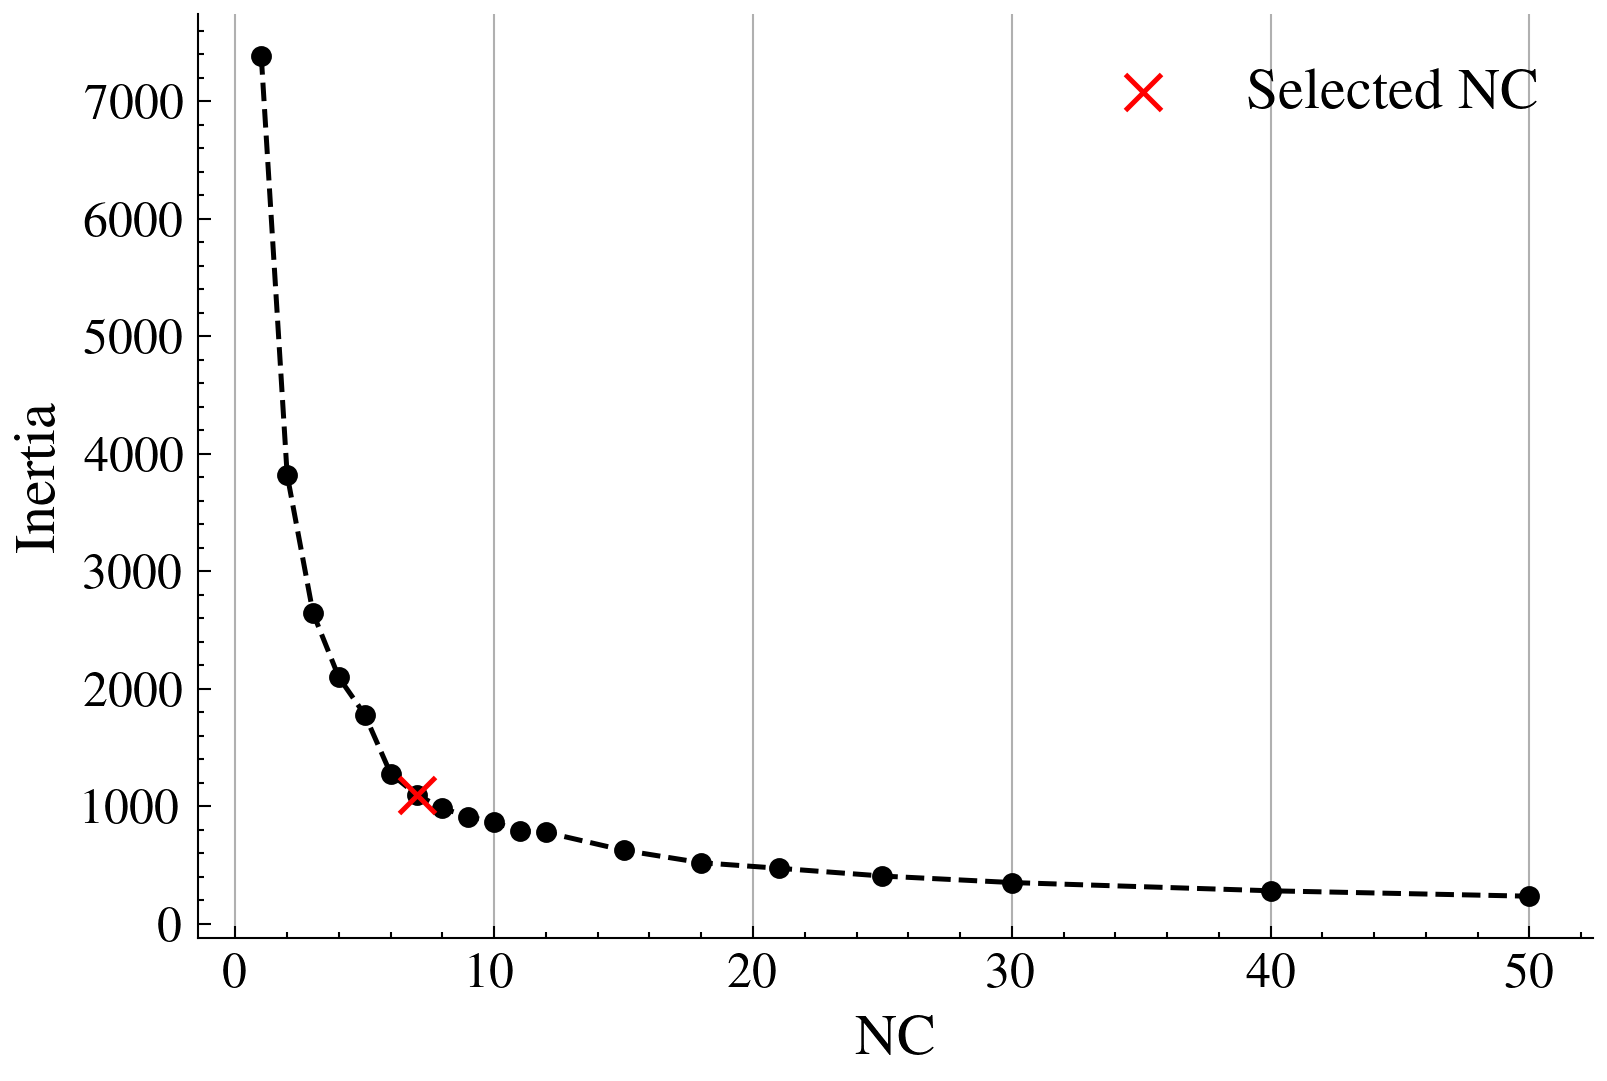
\includegraphics[width=0.6\textwidth]{results/img/elbow_plot.png}
    \caption{Elbow chart for the clustering.}
    \label{fig:elbow_chart}
\end{figure}
The plot shows a clear elbow near $K=7$, which is thus chosen as the optimal number of clusters.
Once all the parameters of the clustering are defined, the clustering is applied to the whole dataset and the results are shown in Fig.~\ref{fig:clustering_results_tot}.
\begin{figure}[h]
    \centering
    \begin{subfigure}{0.49\textwidth}
        \centering
        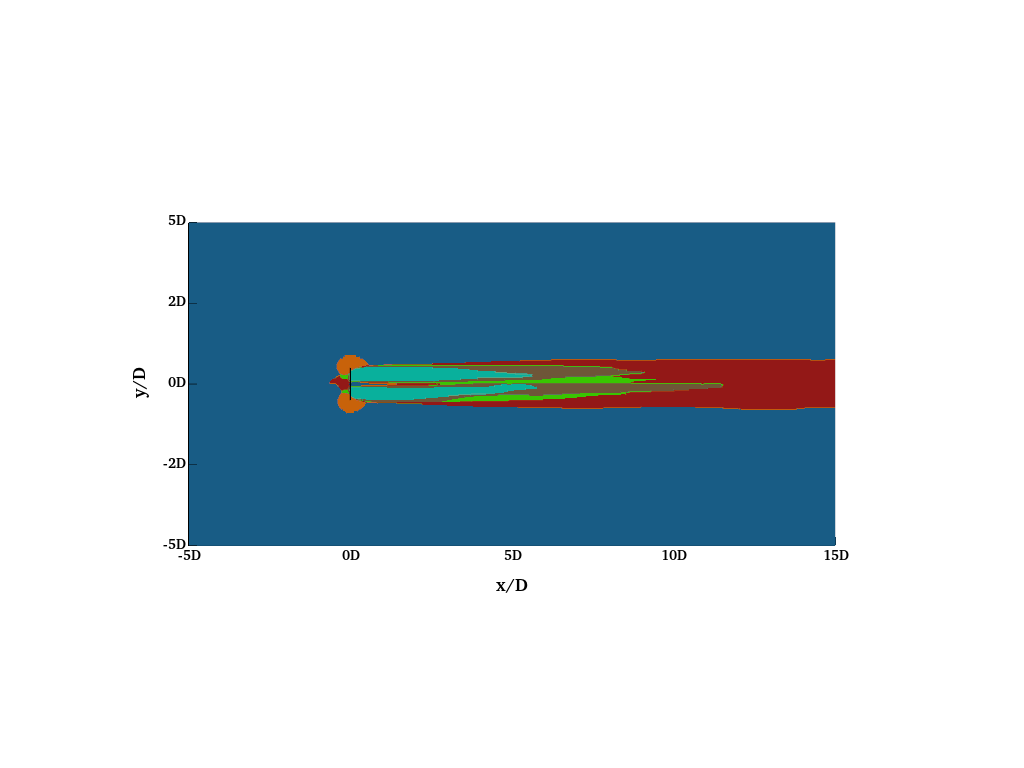
\includegraphics[width=\textwidth, trim=80 120 80 150, clip=true]{results/img/clustering_result_xy.png}
        \caption{}
        \label{fig:clustering_results}
    \end{subfigure}
    \hfill
    \begin{subfigure}{0.49\textwidth}
        \centering
        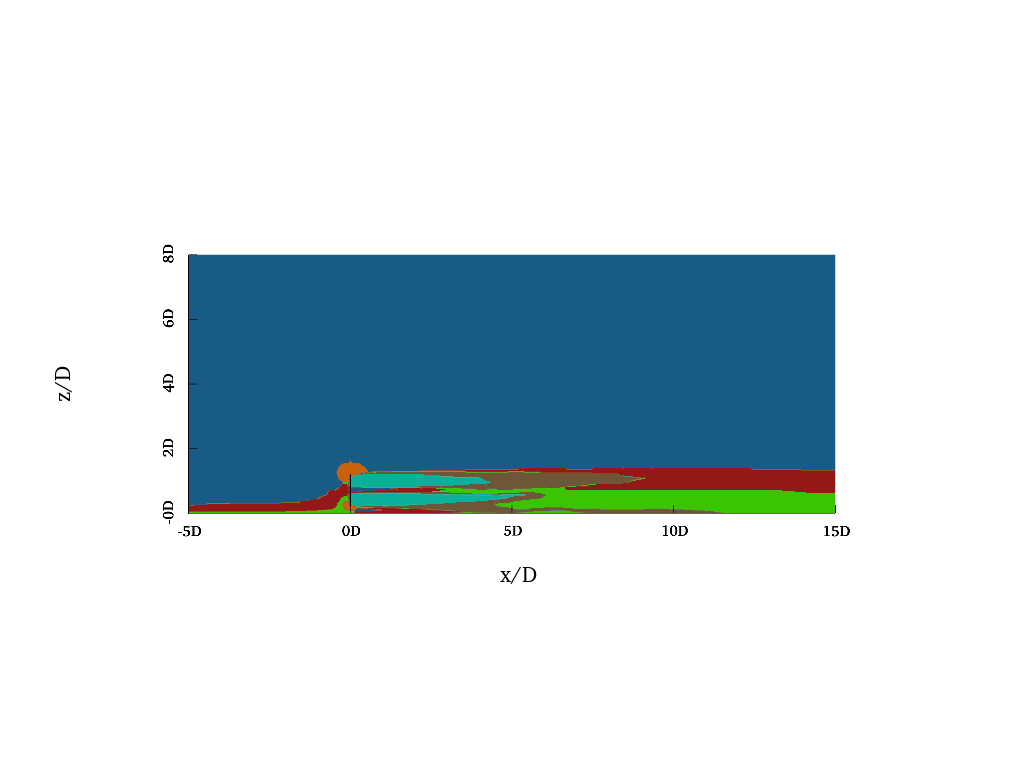
\includegraphics[width=\textwidth, trim=80 120 80 150, clip=true]{results/img/clustering_result_xz.png}
        \caption{}
        \label{fig:clustering_results_xz}
    \end{subfigure}
    \begin{subfigure}{0.6\textwidth}
        \centering
        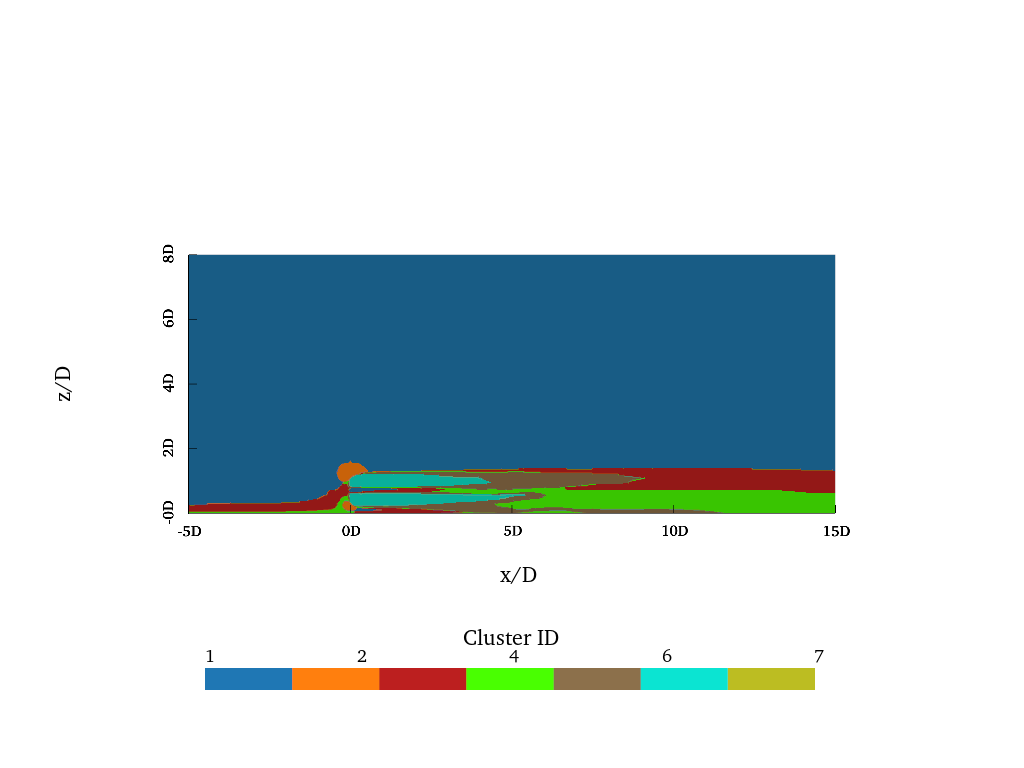
\includegraphics[width=\textwidth, trim=190 50 190 600, clip=true]{results/img/clustering_result_legend.png}
        \label{fig:clustering_results_legend}
    \end{subfigure}
    \caption{Clustering results: (a) xy view, (b) xz view.}
    \label{fig:clustering_results_tot}
\end{figure}
Different regions of the flow are clearly identified by the clustering. A clear separation between the disturbed and undisturbed flow can be seen:
\begin{itemize}
    \item Cluster 1 identifies the undisturbed flow.
    \item Clusters from 2 to 7 identify wake. In particular, cluster 3 identifies the inlet-ABL-affected region upstream of the rotor and the upper far-wake region; cluster 4 identifies the lower ABL-influenced far-wake region; the near-wake is identified by cluster 6, while cluster 5 highlights the near-wake region with higher $k$ levels and the mixing/breakdown region; finally, cluster 7 identifies the upstream rotor-inlet region.
\end{itemize}
Clusters validation is performed as in \cite{Carloni2026} and will not be shown here for brevity but the results are consistent with the reference and with the physical phenomena occurring in the flow. The clustering results are thus considered valid and the clusters are used for the training of the ML-based RANS model.
Clustering model is trained in $\sim 0.24$ seconds on the previously defined workstation and dataset.

\subsection{NN results}
\label{sec:NN_results}
The NN model is trained using the fixed manual configuration described in Sec.~\ref{sec:ML_part}.

The network predicts the standardised correction $\Delta \nu_t=\nu_{t,eq}-\nu_{t,\mathrm{RANS}}$ and the final eddy viscosity is reconstructed as $\nu_{t,ML}=\nu_{t,\mathrm{RANS}}+\Delta \nu_{t,ML}$. In the reported run, trained on the $U_\infty=11\,\mathrm{m/s}$ operating condition, the best checkpoint is obtained at epoch 220, where $validation\ loss=2.47\cdot10^{-2}$ and $validation\ MAE=2.86\cdot10^{-2}$ in normalized target space. On the training set the reconstructed physical field reaches $R^2=0.9954$, $RMSE=0.2584$ and $MAE=0.1769$, while the validation subset gives $R^2=0.9952$, $RMSE=0.2635$ and $MAE=0.1797$.

The training and validation loss curves are shown in Fig.~\ref{fig:training_curves} as also the scatter plot of the predicted and true $\nu_t$ values on the test set.
\begin{figure}
    \centering
    \begin{subfigure}{0.32\textwidth}
        \centering
        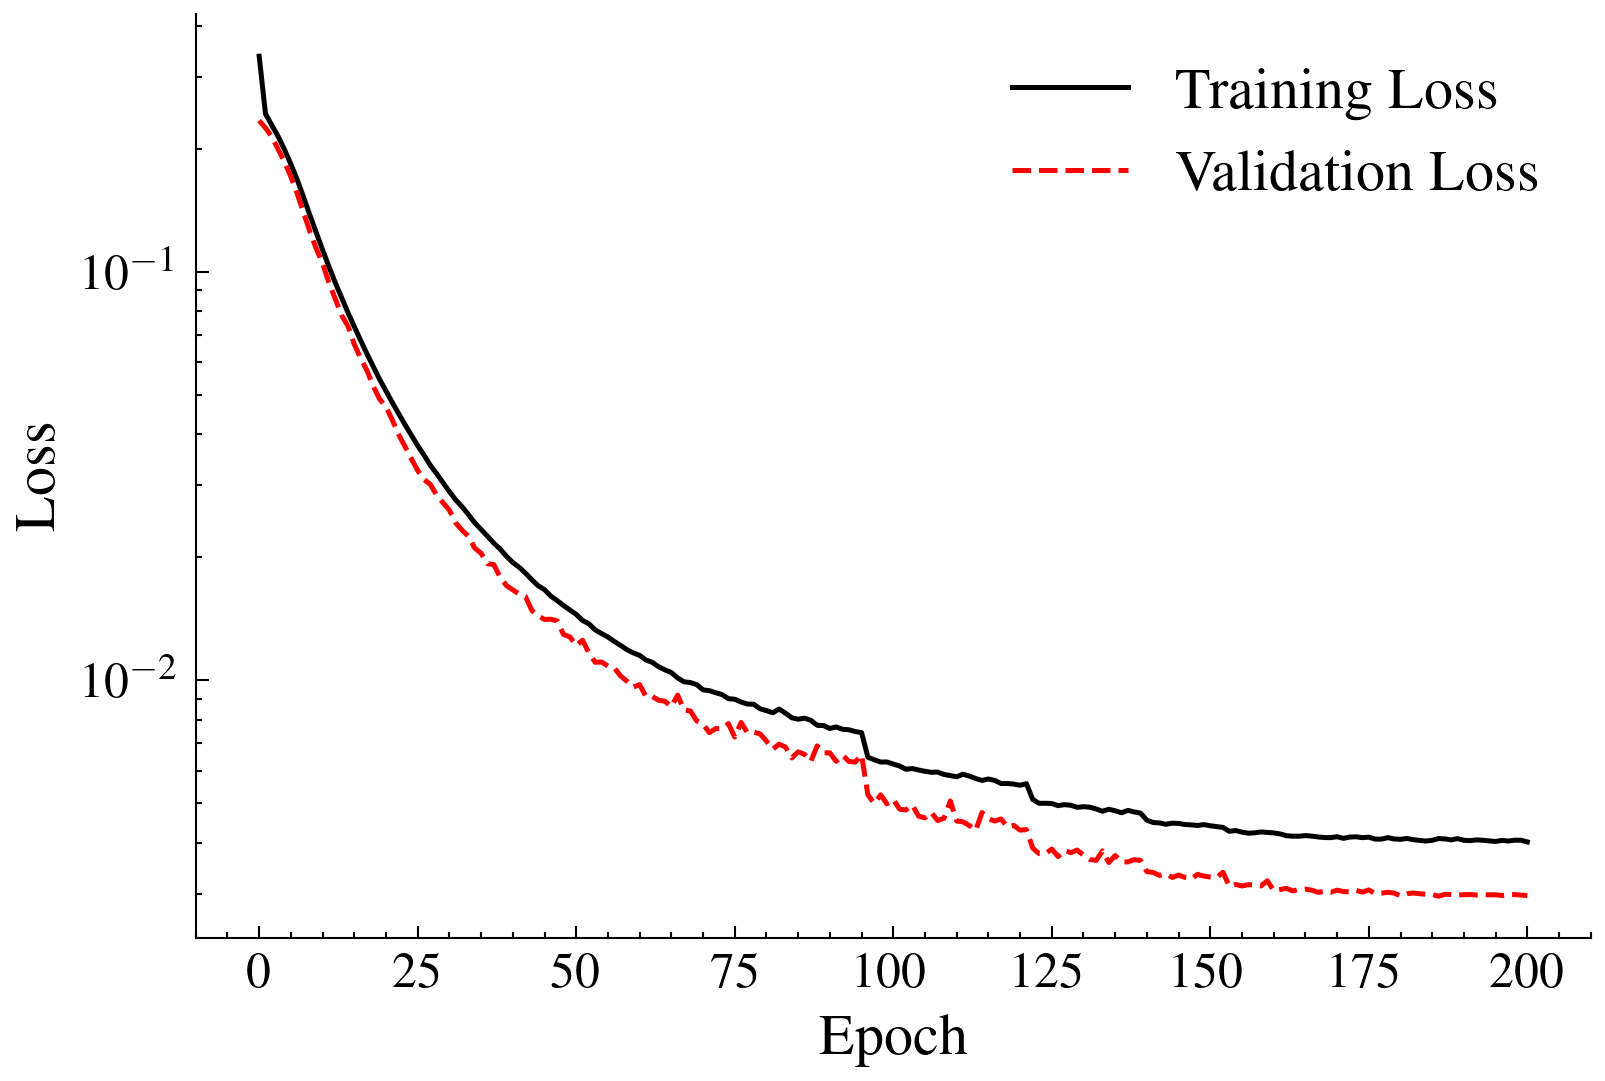
\includegraphics[width=\textwidth]{results/img/NN_loss_curves.png}
        \caption{}
        \label{fig:NN_loss_curves}
    \end{subfigure}
    \hfill
    \begin{subfigure}{0.32\textwidth}
        \centering
        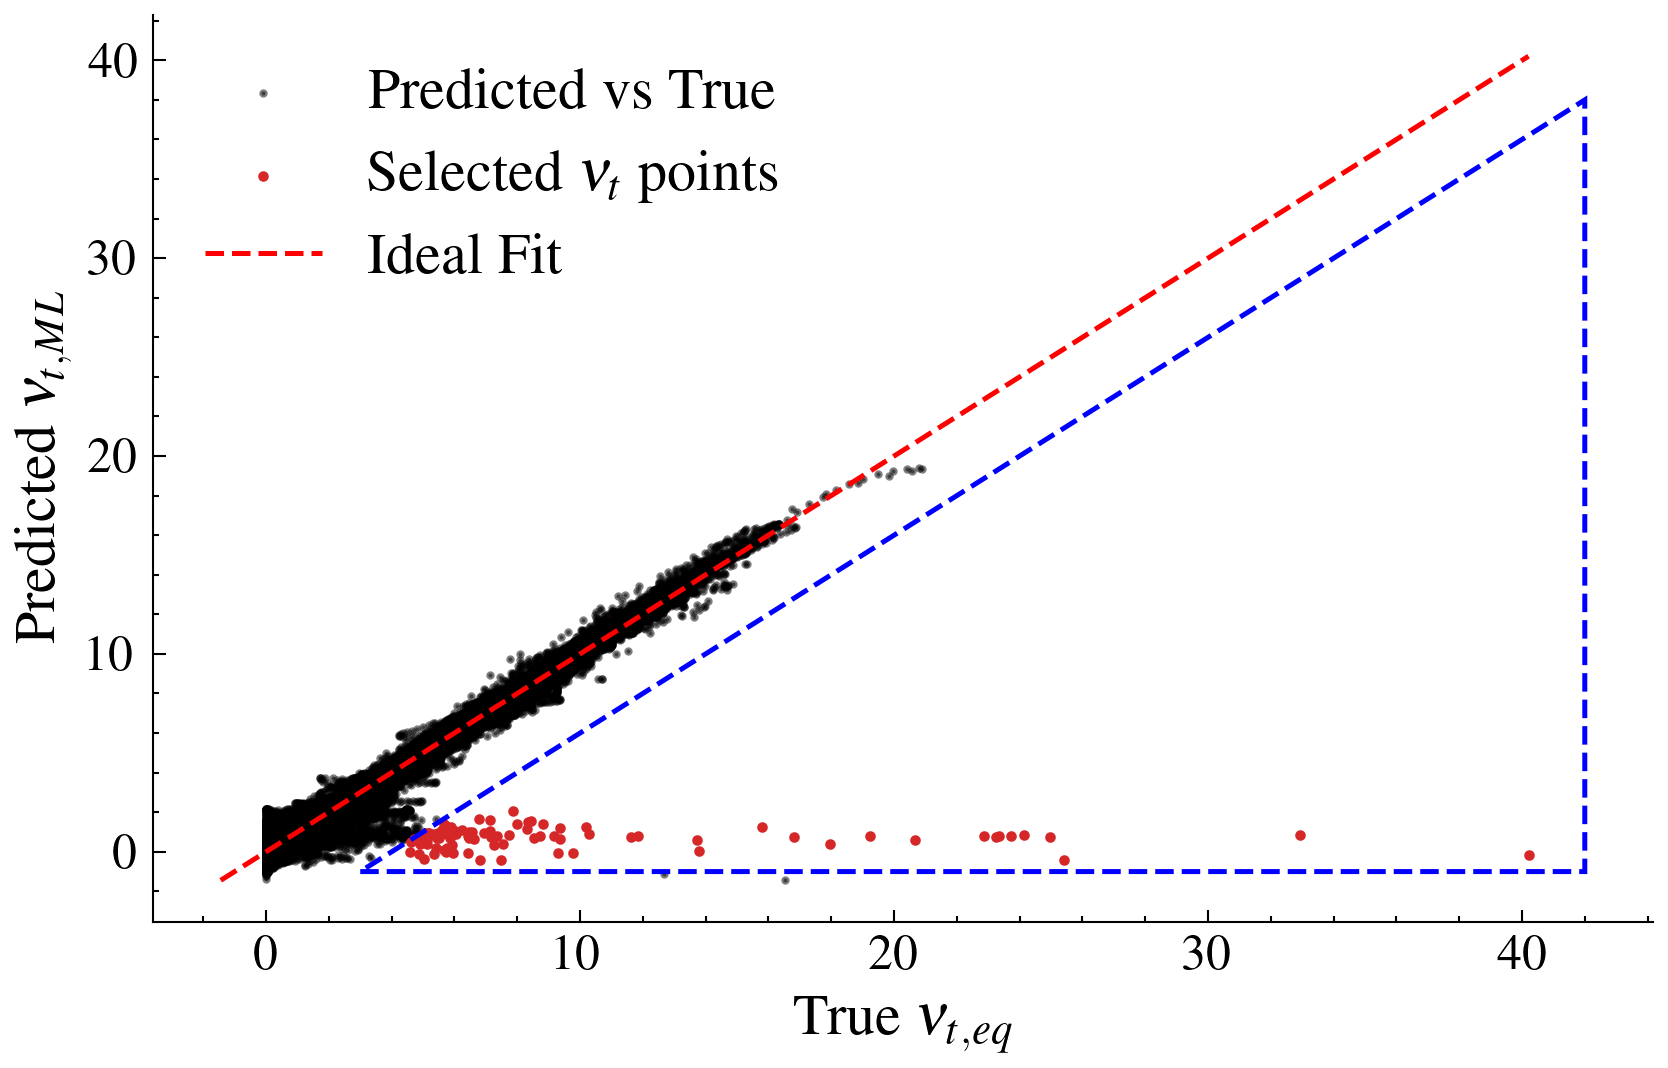
\includegraphics[width=\textwidth]{results/img/ml_results/bias_points/nut_scatter_bias_points_highlighted.png}
        \caption{}
        \label{fig:NN_scatter_plot}
    \end{subfigure}
    \hfill
    \begin{subfigure}{0.32\textwidth}
        \centering
        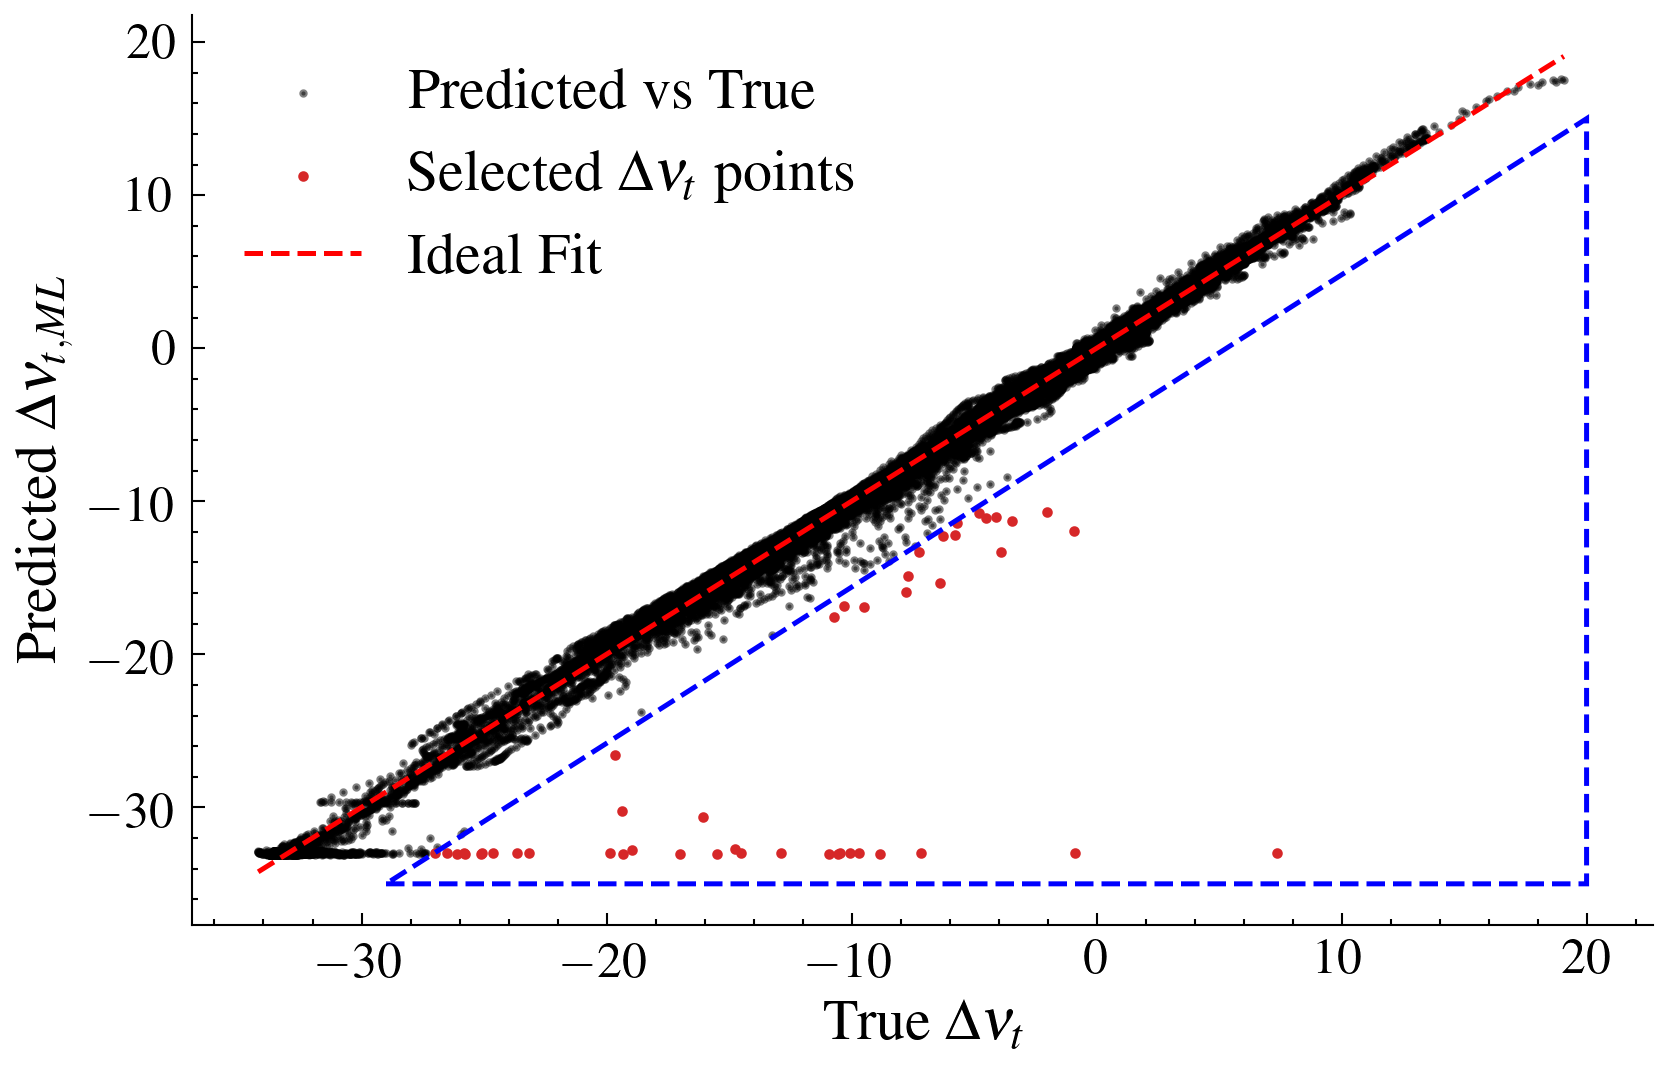
\includegraphics[width=\textwidth]{results/img/ml_results/bias_points/delta_scatter_bias_points_highlighted.png}
        \caption{}
        \label{fig:NN_delta_scatter_plot}
    \end{subfigure}
    \begin{subfigure}{0.5\textwidth}
        \centering
        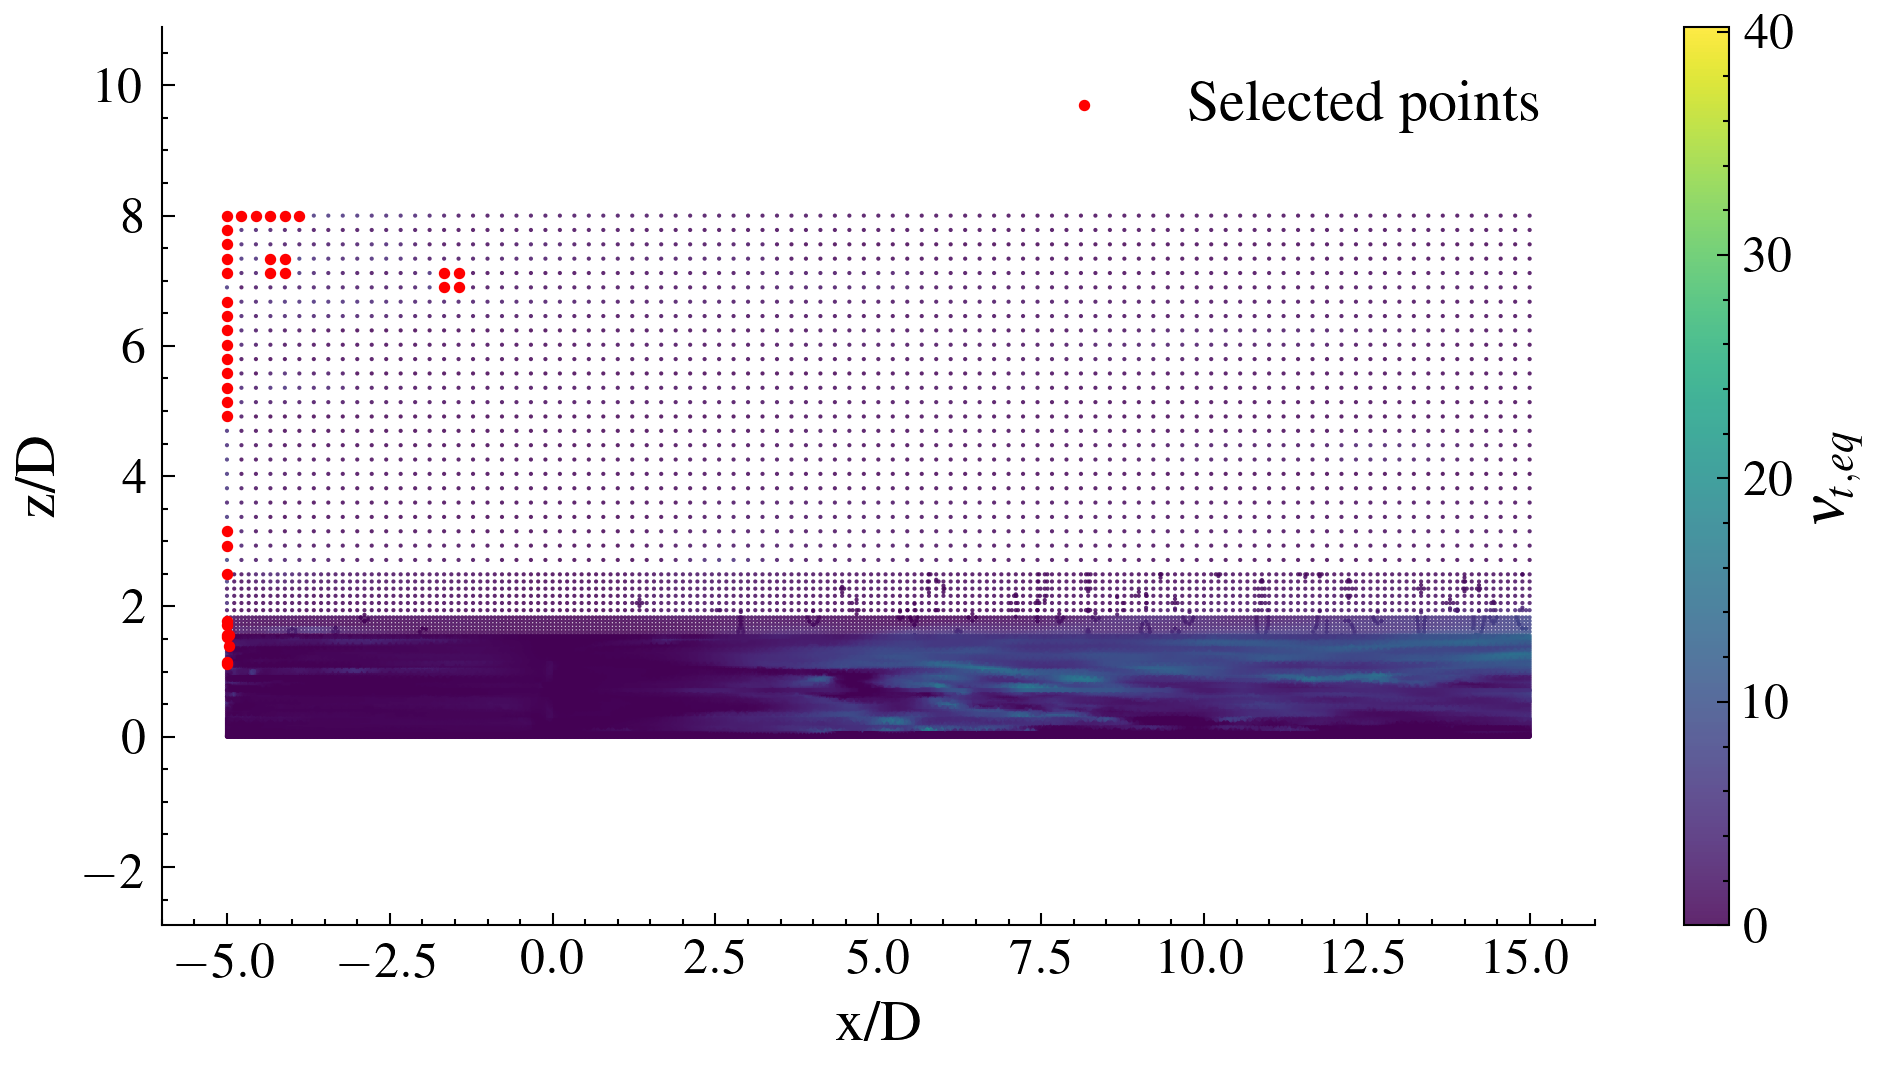
\includegraphics[width=\textwidth]{results/img/ml_results/bias_points/delta_bias_points_on_y0_slice.png}
        \caption{}
        \label{fig:NN_scatter_plot_legend}        
    \end{subfigure}
    \caption{NN results: (a) training and validation loss curves, (b) scatter plot of predicted vs true $\nu_t$ values on the test set, (c) scatter plot of predicted vs true $\Delta \nu_t$ values on the test set, (d) slice plot of selected high-error points.}
    \label{fig:training_curves}
\end{figure}
From Fig.~\ref{fig:NN_loss_curves} a small gap between the training and validation loss can be observed, consistent with the deliberately compact training set, which by design consists of a single operating condition ($U_\infty=11\,\mathrm{m/s}$) sampled on a single grid. This gap is the expected price of the single-case calibration that is central to the methodology, and it does not compromise the predictive use of the closure: the two curves do not diverge, the validation metrics are essentially identical to the training ones ($R^2=0.995$ in both), and, as shown in Sec.~\ref{sec:generalization}, the embedded model transfers accurately to grids and inflow velocities outside the training set. Accordingly, the NN predictions are accurate, as shown in Fig.~\ref{fig:NN_scatter_plot}, where the predicted $\Delta \nu_{t,ML}$ values are close to the true $\Delta \nu_{t}$ values, as also happens in Fig.~\ref{fig:NN_delta_scatter_plot}, where the predicted $\nu_{t,ML}$ values are close to the true $\nu_{t,eq}$ values. A series of outliers can be noted in the predictions, in the marked region of the scatter plots, where the NN underestimates the true $\nu_{t,eq}$ values. This is inherited from the same bias area highlighted in the scatter plot of the $\Delta \nu_{t,ML}$ values, where the NN underestimates the true $\Delta \nu_t$ values. This, as Fig.~\ref{fig:NN_scatter_plot_legend} shows, corresponds to a specific region of the domain, located at the inlet, in which numerical instabilities are present due to the coded inlet boundary condition. In such area the NN predictions are less accurate, but this is not expected to significantly affect the overall performance of the ML-based RANS model.
In fact, the NN predictions are still accurate and the NN-based RANS model is expected to perform better than the standard RANS model, as shown in the next section. The resulting $\nu_{t,ML}$ field is shown in Fig.~\ref{fig:nu_t_fields} together with the $\nu_{t,eq}$ and $\nu_{t,\mathrm{RANS}}$ fields for comparison.
\begin{figure}
    \centering
    \begin{subfigure}{0.32\textwidth}
        \centering
        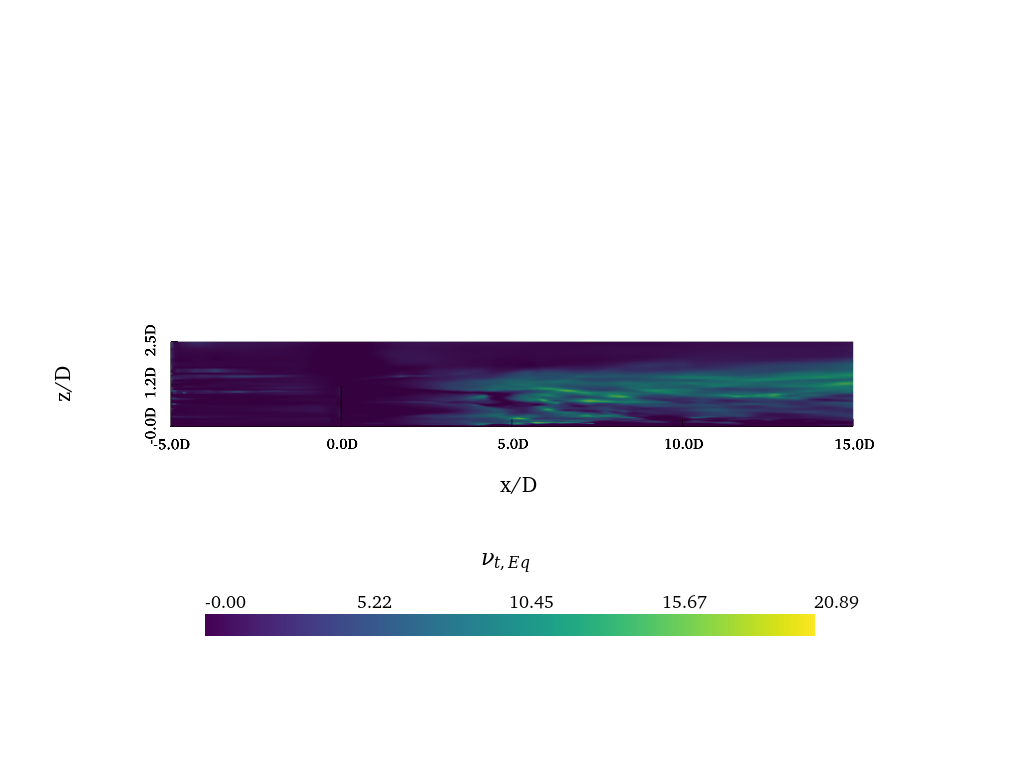
\includegraphics[width=\textwidth, trim=80 120 80 150, clip=true]{results/img/nutEq_field_xz.png}
        \caption{}
        \label{fig:nu_t_eq}
    \end{subfigure}
    \hfill
    \begin{subfigure}{0.32\textwidth}
        \centering
        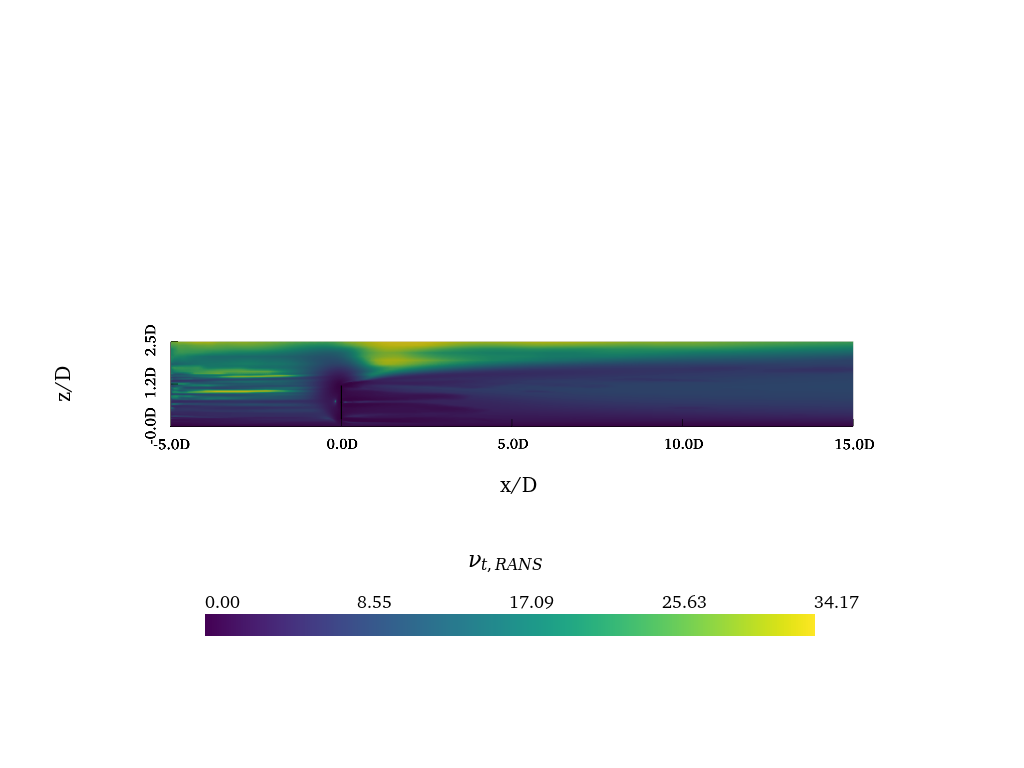
\includegraphics[width=\textwidth, trim=80 120 80 150, clip=true]{results/img/nut_rans_field_xz.png}
        \caption{}
        \label{fig:nu_t_RANS}
    \end{subfigure}
    \hfill
    \begin{subfigure}{0.32\textwidth}
        \centering
        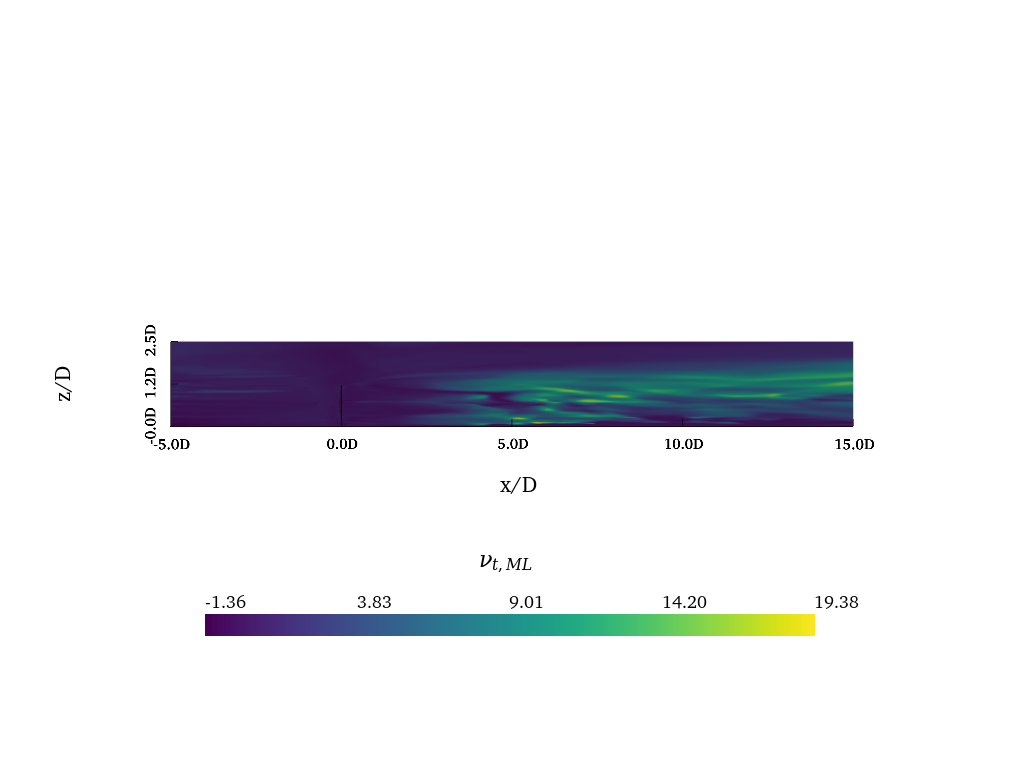
\includegraphics[width=\textwidth, trim=80 120 80 150, clip=true]{results/img/nut_pred_field_xz.png}
        \caption{}
        \label{fig:nu_t_ML}
    \end{subfigure}
    \caption{Eddy viscosity fields: (a) $\nu_{t,eq}$, (b) $\nu_{t,\mathrm{RANS}}$ (obtained by importing the mean pressure and velocity field of the LES in the RANS solver), (c) $\nu_{t,ML}$.}
    \label{fig:nu_t_fields}
\end{figure}

\subsection{ML-based RANS model results}
\label{sec:ml_rans_results}
The trained ML model is embedded in the RANS solver as described in Sec.~\ref{sec:ML_part} and evaluated across grids of different resolutions to assess both its predictive accuracy and its computational efficiency.

To highlight the importance of clustering in the methodology, the ML-based RANS model was compared against a variant trained without clustering, using the same network architecture and hyperparameters without all clustering-related components. The best validation loss for the unclustered model is obtained at epoch 219, with $validation\ loss \approx 2.44\cdot10^{-2}$ and $validation\ MAE = 2.95\cdot10^{-2}$ in the normalised target space. On the validation subset, the reconstructed physical field reaches $R^2 = 0.9950$, $RMSE = 0.2713$ and $MAE = 0.1812$. All these metrics are slightly worse than in the clustered case ($R^2 = 0.9952$, $RMSE = 0.2635$, $MAE = 0.1797$), indicating that clustering allows the model to better capture the variance of the data and thus to reconstruct the physical field more faithfully. The aggregate metrics differ only marginally because they are dominated by the large, well-behaved free-stream region; the value of clustering, however, lies not in the global score but in \emph{where} the improvement is concentrated, in its robustness to mesh refinement and in the physical interpretability it provides, as discussed in the following. The training and validation loss curves together with the scatter plots of the predicted and true $\nu_t$ and $\Delta \nu_t$ values on the test set are shown in Fig.~\ref{fig:training_curves_no_clustering}.

\begin{figure}
    \centering
    \begin{subfigure}{0.32\textwidth}
        \centering
        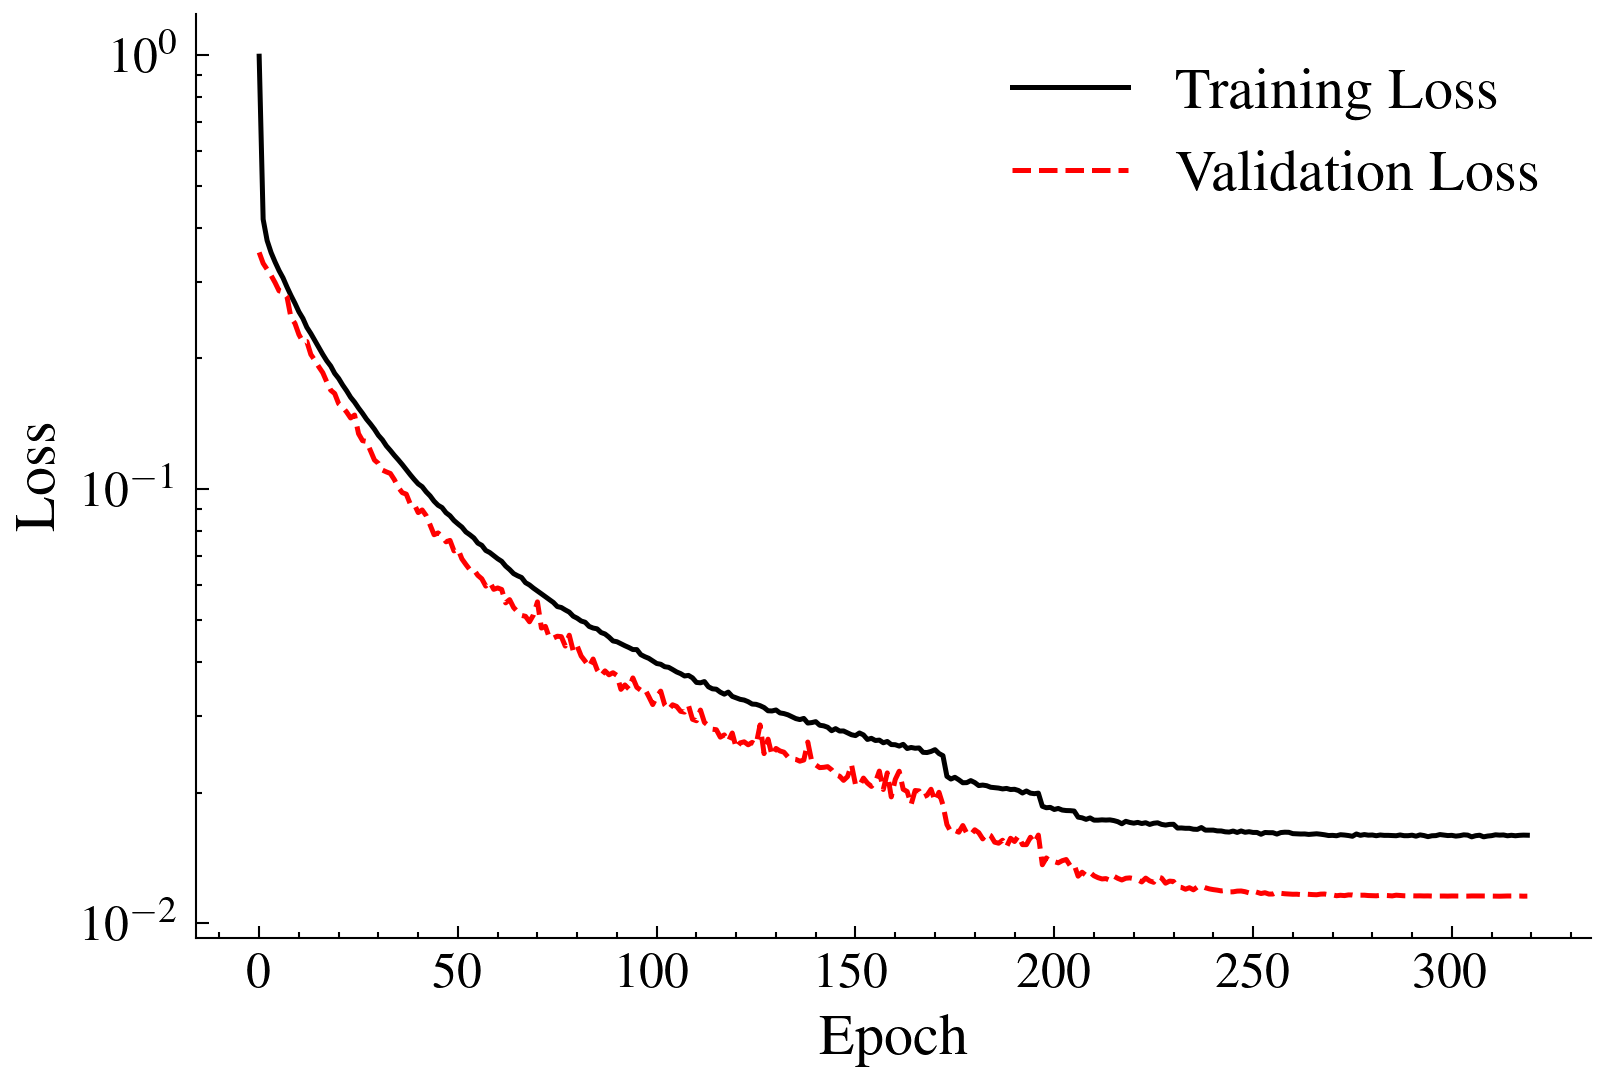
\includegraphics[width=\textwidth]{results/img/NN_loss_curves_no_clustering.png}
        \caption{}
        \label{fig:NN_loss_curves_no_clustering}
    \end{subfigure}
    \hfill
    \begin{subfigure}{0.32\textwidth}
        \centering
        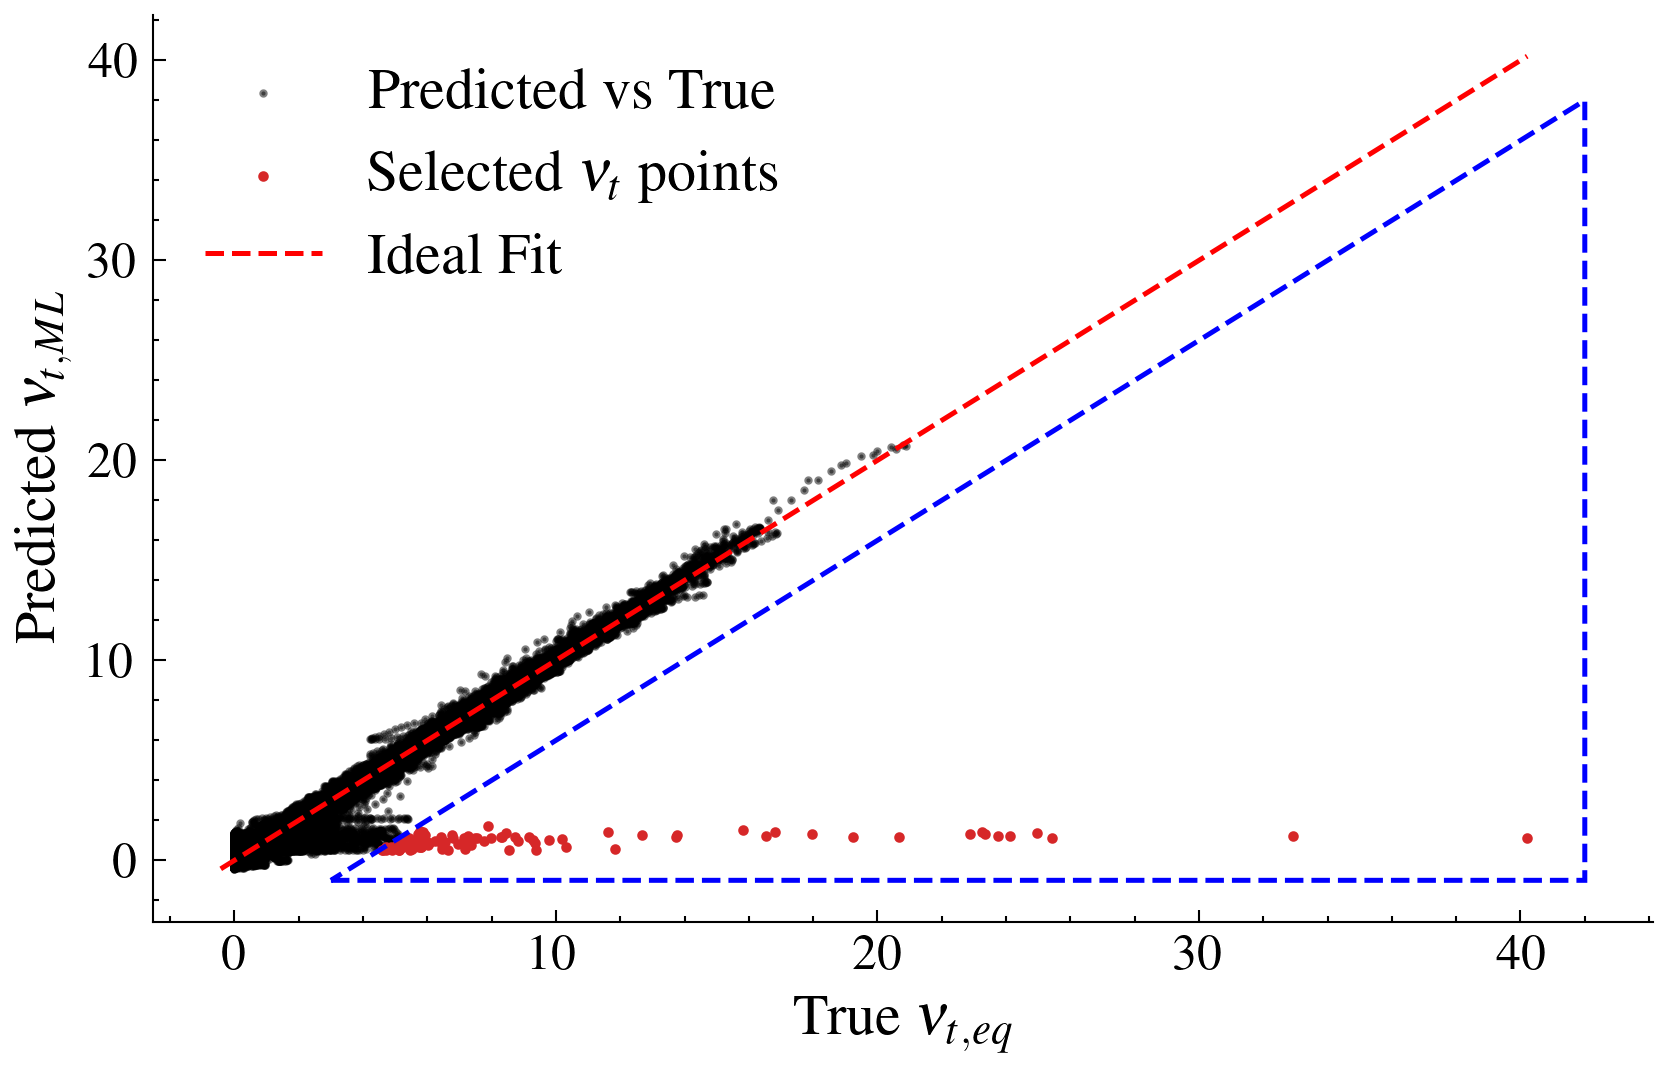
\includegraphics[width=\textwidth]{results/img/ml_results/bias_points/nut_scatter_bias_points_highlighted_no_clustering.png}
        \caption{}
        \label{fig:NN_scatter_plot_no_clustering}
    \end{subfigure}
    \hfill
    \begin{subfigure}{0.32\textwidth}
        \centering
        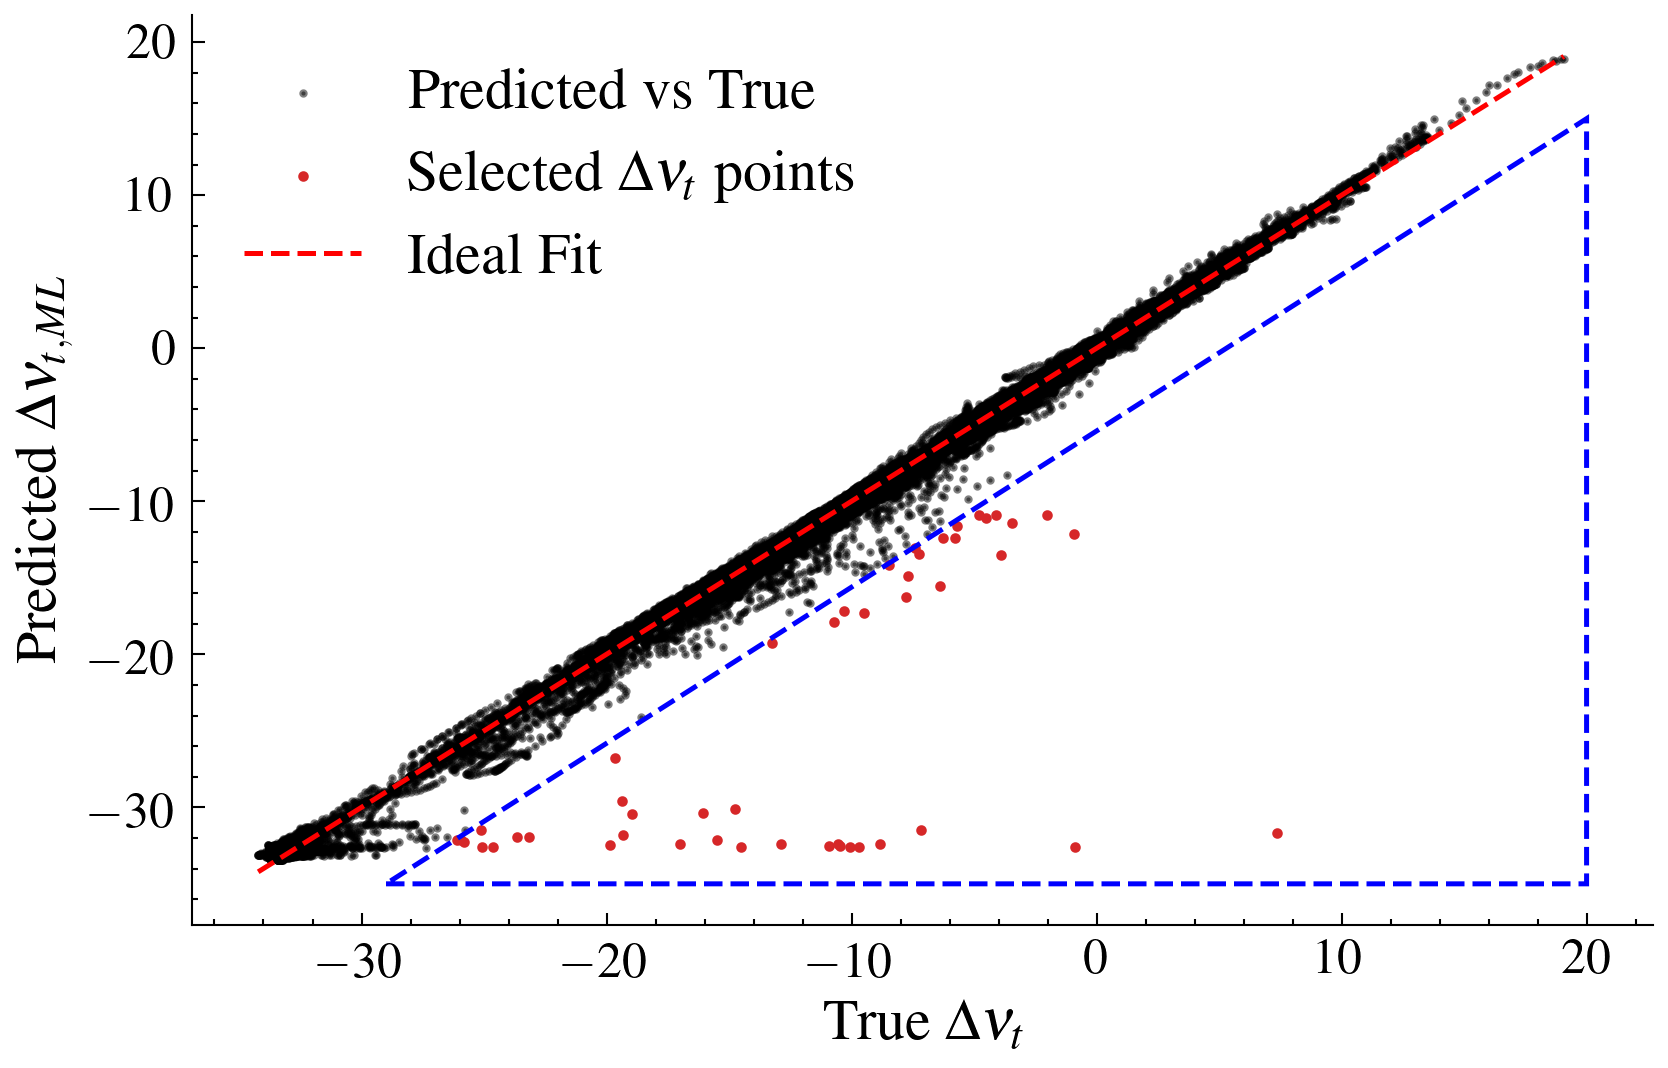
\includegraphics[width=\textwidth]{results/img/ml_results/bias_points/delta_scatter_bias_points_highlighted_no_clustering.png}
        \caption{}
        \label{fig:NN_delta_scatter_plot_no_clustering}
    \end{subfigure}
    \begin{subfigure}{0.5\textwidth}
        \centering
        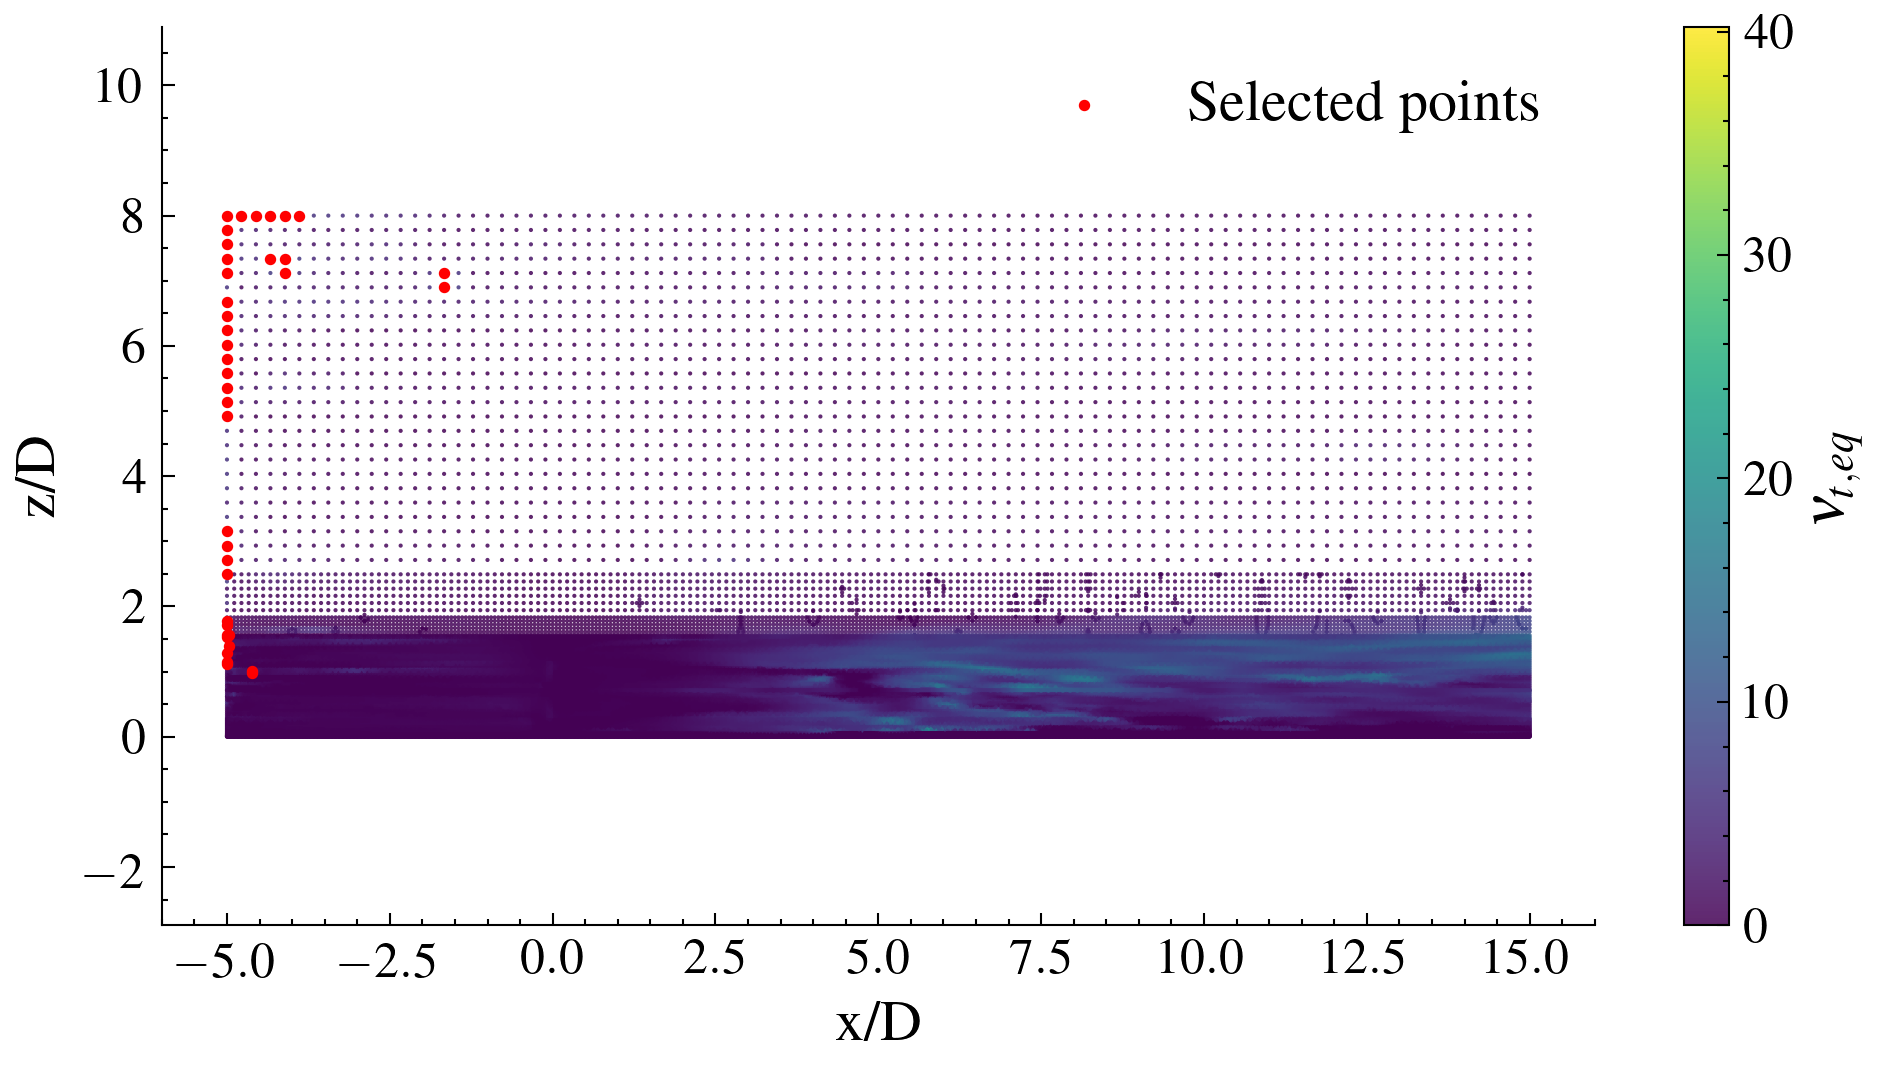
\includegraphics[width=\textwidth]{results/img/ml_results/bias_points/delta_bias_points_on_y0_slice_no_clustering.png}
        \caption{}
        \label{fig:NN_scatter_plot_legend_no_clustering}        
    \end{subfigure}
    \caption{NN results of the model without clustering: (a) training and validation loss curves, (b) scatter plot of predicted vs true $\nu_t$ values on the test set, (c) scatter plot of predicted vs true $\Delta \nu_t$ values on the test set, (d) slice plot of selected high-error points.}
    \label{fig:training_curves_no_clustering}
\end{figure}

As visible in Figures \ref{fig:NN_scatter_plot_no_clustering} and \ref{fig:NN_delta_scatter_plot_no_clustering}, the unclustered model exhibits the same underestimation bias in the inlet region as well as a slightly overfitting trend. More importantly, the absence of clustering leads to a degraded prediction in the near-terrain region, where the flow is strongly influenced by the ground boundary layer and exhibits high spatial variability. In this zone the clustered model produces results that are considerably more consistent with the LES reference, since clustering enables the network to learn separately the distinct flow regimes present in the near-wall and free-stream regions, rather than approximating them with a single global mapping.

Finally, the ML-based RANS model results are shown in Fig.~\ref{fig:ml_results}.

\begin{figure}
    \centering
    \begin{subfigure}{\textwidth}
        \centering
        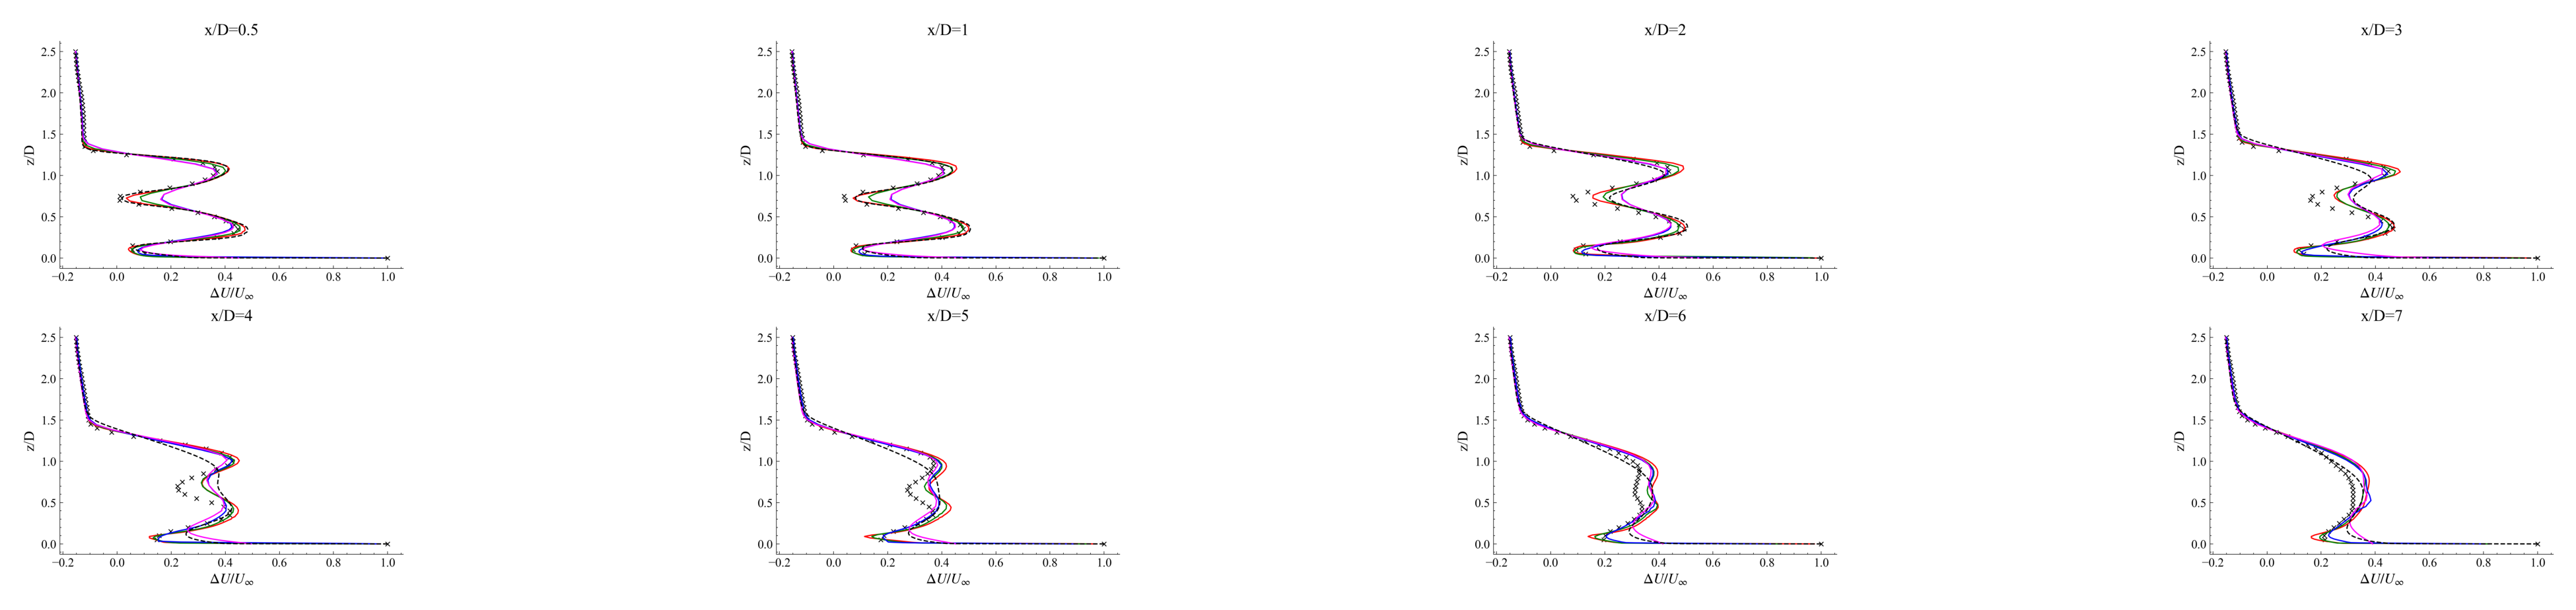
\includegraphics[width=\textwidth]{results/img/ml_results/11ms/deficit/ml_models_comparison/velocity/comparison.png}
        \caption{}
        \label{Fig:velocity_deficit}        
    \end{subfigure}
    \begin{subfigure}{0.3\textwidth}
        \centering
            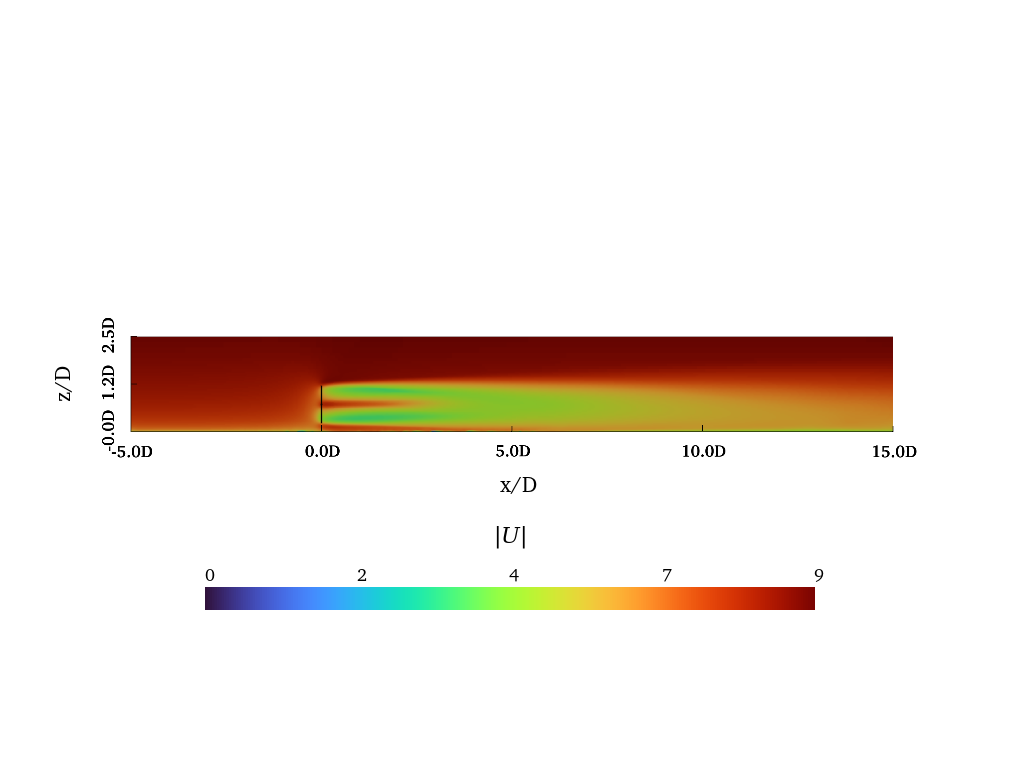
\includegraphics[width=\textwidth, trim=80 120 80 150, clip=true]{results/img/predicted_U_field_xz.png}
            \caption{}
        \label{Fig:velocity_plot}
    \end{subfigure}
    \begin{subfigure}{0.3\textwidth}
        \centering
        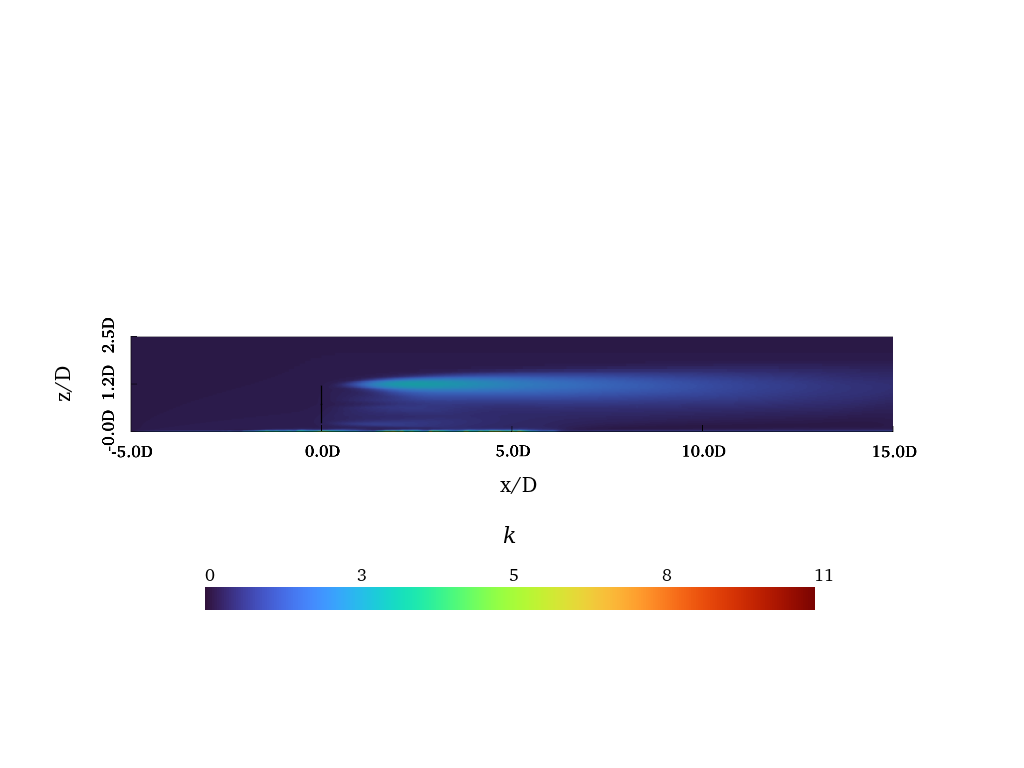
\includegraphics[width=\textwidth, trim=80 120 80 150, clip=true]{results/img/predicted_k_field_xz.png}
        \caption{}
        \label{Fig:k_plot}
    \end{subfigure}
    \begin{subfigure}{0.3\textwidth}
        \centering
        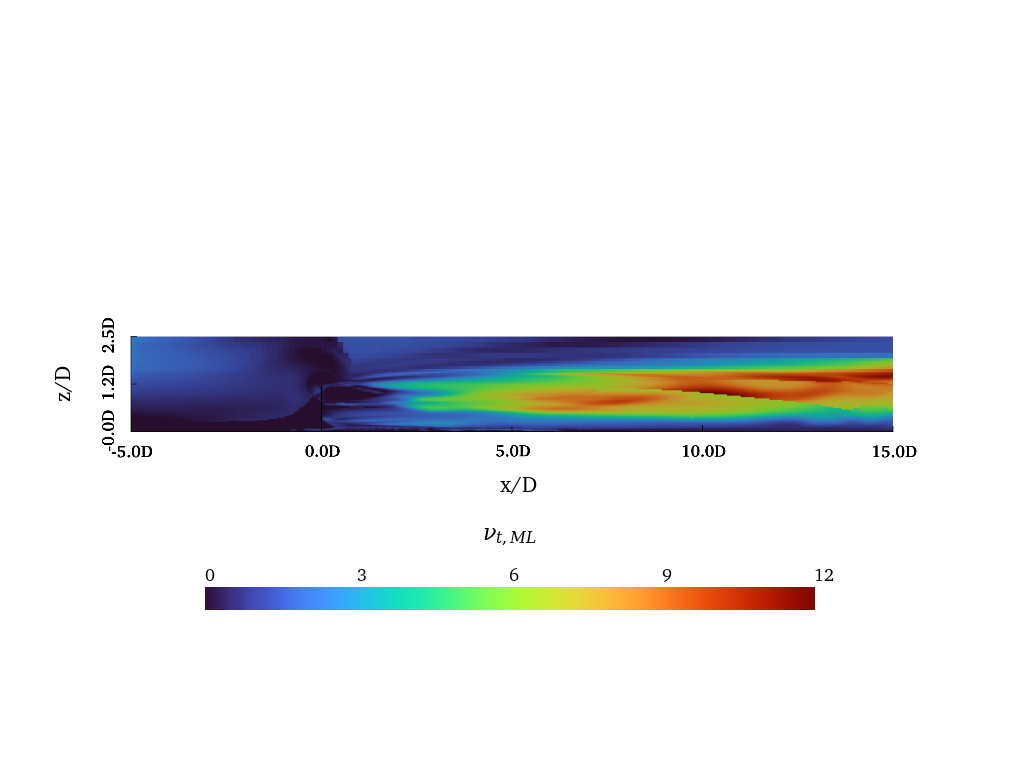
\includegraphics[width=\textwidth, trim=80 120 80 150, clip=true]{results/img/predicted_nut_field_xz.png}
        \caption{}
        \label{Fig:nut_plot}
    \end{subfigure}
    \caption{ML-based RANS model results: (a) velocity deficit along the x-axis at different streamwise distances from the rotor, (b) velocity field, (c) $k$ field, (d) $\nu_{t,ML}$ field.}
    \label{fig:ml_results}
\end{figure}

Velocity deficit along the x-axis at different streamwise distances from the rotor (Fig.~\ref{Fig:velocity_deficit}) is compared, on grids of different resolution, with the standard RANS model and with the LES reference, together with the predicted velocity, turbulent kinetic energy and eddy viscosity fields (Figures \ref{Fig:velocity_plot}-\ref{Fig:nut_plot}).

On the fine grid ($\sim 15.9$ million cells), the ML-based RANS model consistently outperforms the standard RANS model throughout the wake. In the near-wake region the model shows markedly improved agreement with the LES results, especially in the upper region of the wake where the standard RANS model underestimates the velocity deficit. A moderate underestimation of the velocity deficit persists in the lower near-wake region, attributable to a local underestimation of the $\nu_t$. In the far-wake region, after the breakdown of the wake (i.e., from $4D$ in the streamwise direction), the fine-grid model tends to overestimate the velocity deficit with respect to the LES reference, suggesting that at this resolution the $\nu_t$ correction does not fully reproduce the turbulent mixing responsible for wake recovery.

In terms of computational cost, on the $\sim 15.9$ million cells grid the ML-based RANS model is about $2.5$ times more expensive than the reference LES. This figure should not be read as a drawback of the method: the fine grid is not the deployment configuration but the most refined one, retained here only to characterise the accuracy of the closure at high resolution. At this resolution the unsteady time-marching, combined with the per-iteration clustering and network inference, makes the run more expensive than the LES, so the fine-grid comparison is meaningful for accuracy but not for efficiency. The fair efficiency comparison, and the practical advantage of the methodology, emerges on the coarse grids, where LES-quality far-wake accuracy is obtained at a fraction of the LES cost.

The most significant, and practically relevant, result is obtained on the ultra-coarse grids. As shown in Fig.~\ref{Fig:velocity_deficit}, the ML-based RANS model retains its improved near-wake prediction (with lower accuracy with respect to finer grids) while, at the same time, providing a much more accurate description of the far-wake region, including the post-breakdown zone where the fine-grid model overestimates the deficit. This behaviour makes the ultra-coarse configuration the most attractive option for wind farm applications, where an accurate far-wake prediction is critical to estimate the power production of the downstream turbines and to optimise the wind farm layout. The advantage is further reinforced by the reduction in computational cost: on the $\sim 4.2$ million cells grid the ML-based RANS model is about $1.25$ times cheaper than the standard LES, making it a viable tool for large-scale wind farm simulations that require both accuracy and affordability.

Finally, the error in the velocity field is shown in Fig.~\ref{fig:velocity_error_5m} compared to the standard LES model.
\begin{figure}
    \centering
    \begin{subfigure}{0.49\textwidth}
        \centering
        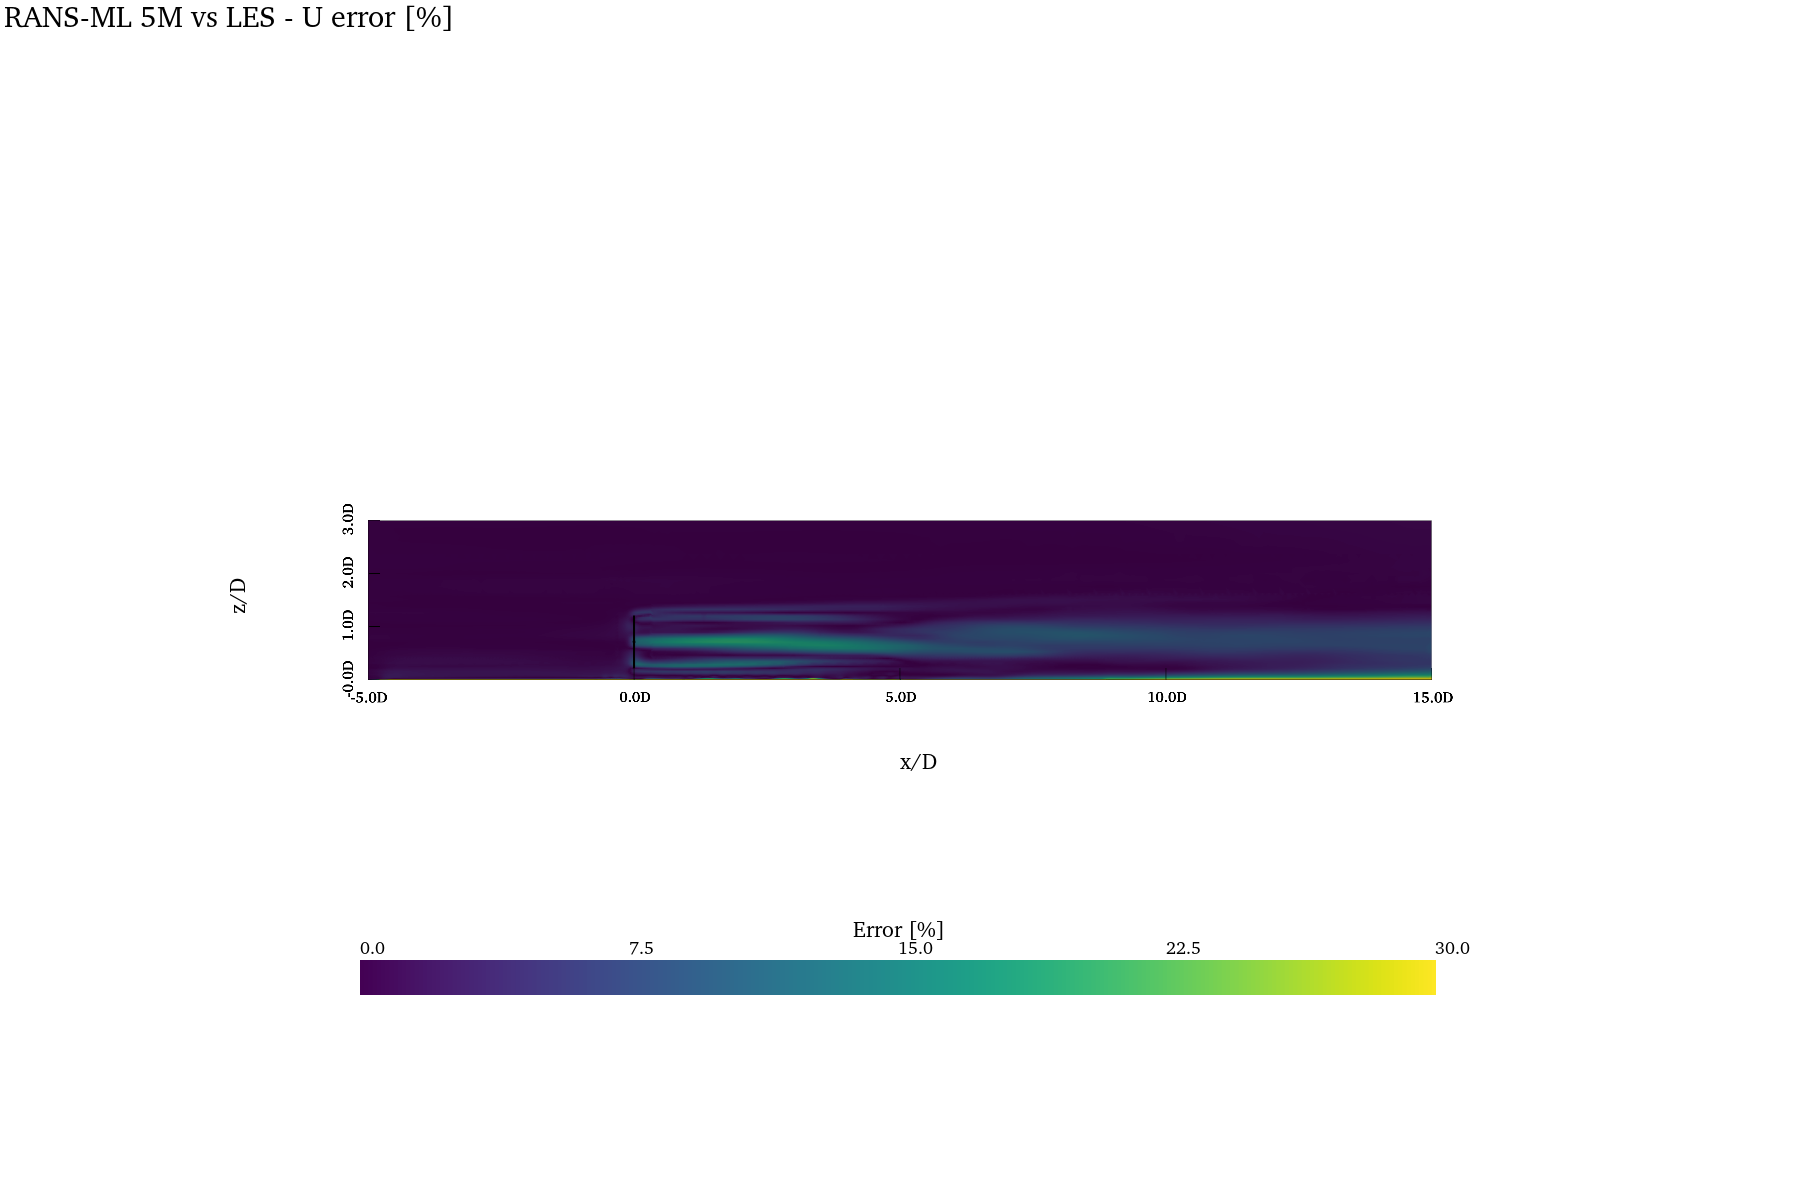
\includegraphics[width=\textwidth, trim=80 120 80 150, clip=true]{results/img/ml_results/11ms/error_fields/rans_ml_5m_vs_les/error_U.png}
        \caption{}
        \label{fig:velocity_error_field_5m}
    \end{subfigure}
    \hfill
    \begin{subfigure}{0.49\textwidth}
        \centering
        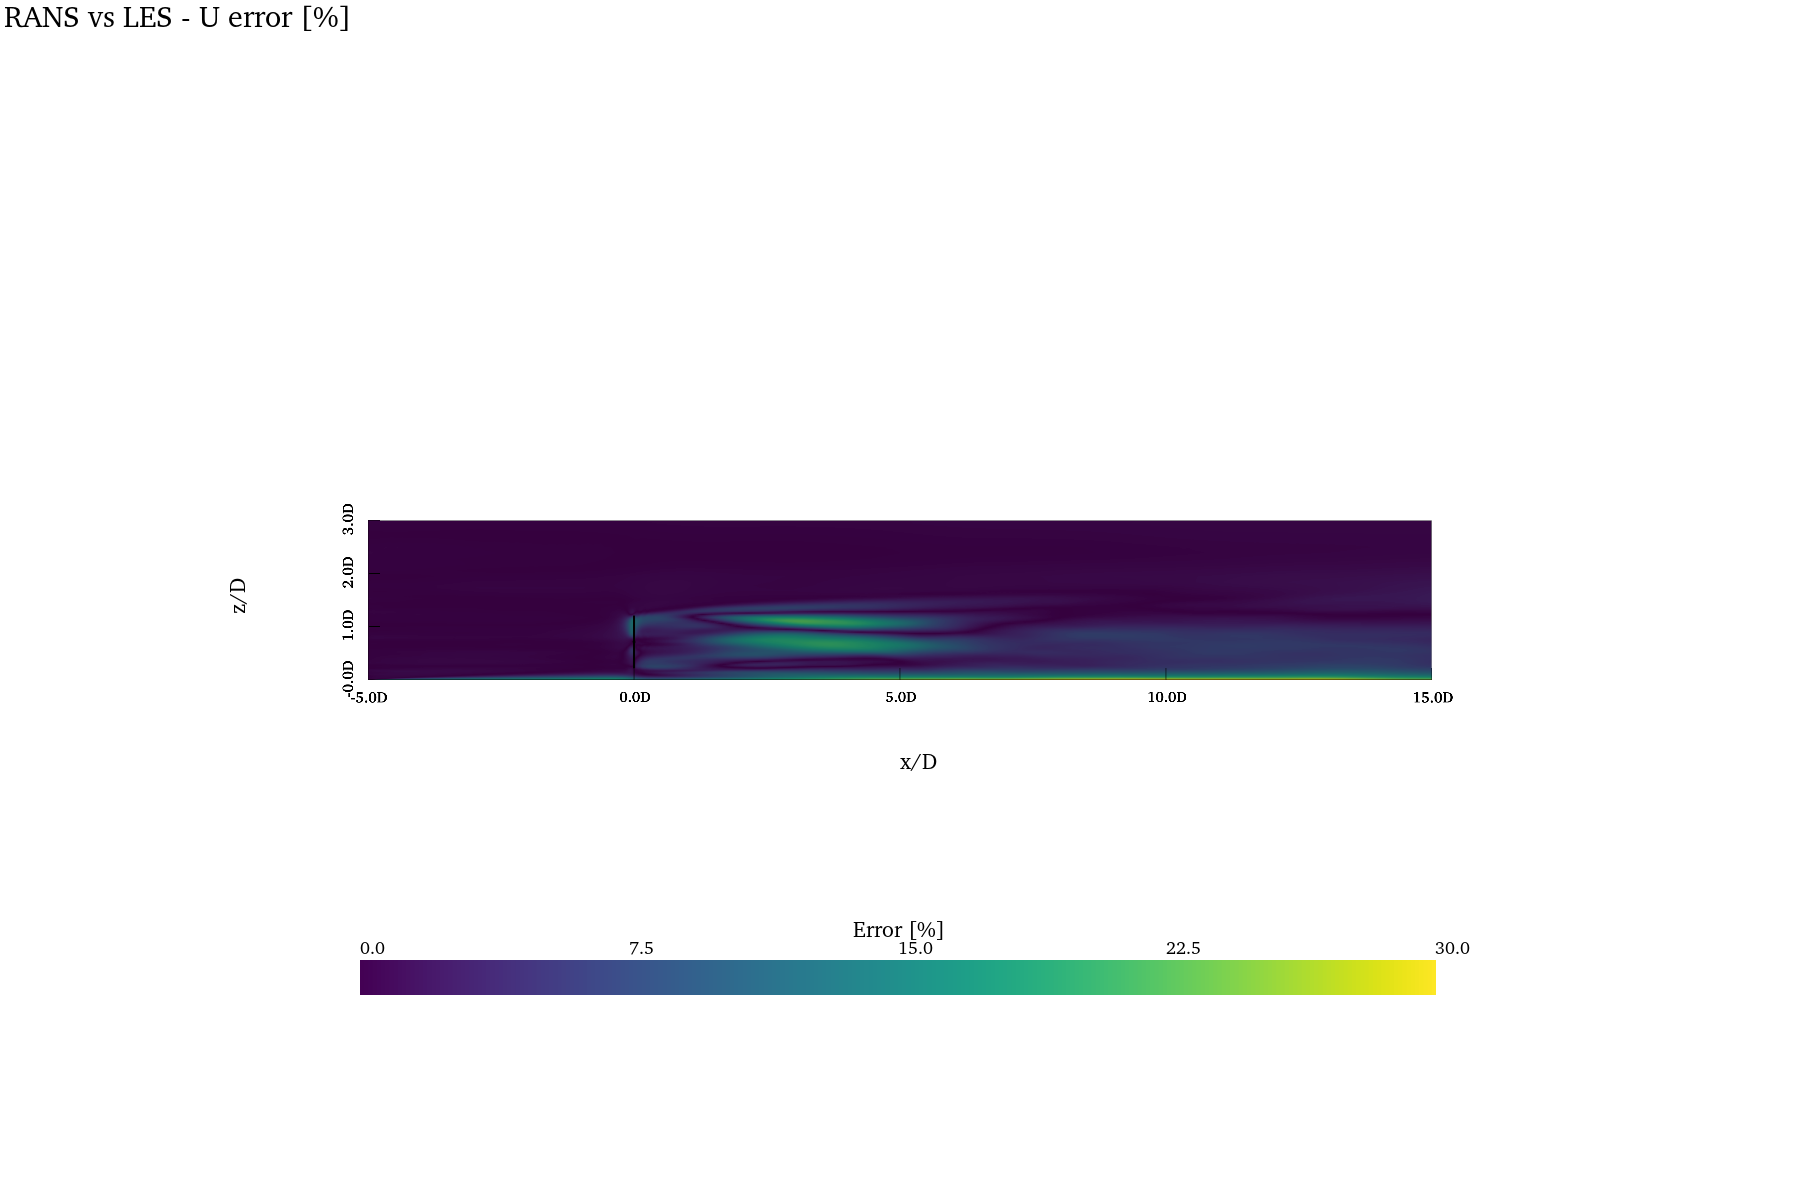
\includegraphics[width=\textwidth, trim=80 120 80 150, clip=true]{results/img/ml_results/11ms/error_fields/rans_vs_les/error_U.png}
        \caption{}
        \label{fig:velocity_error_field_RANS}
    \end{subfigure}
    \caption{Velocity error field of the ML-based RANS model compared to the standard LES model (a) and of RANS one compared to the standard LES model (b).}
    \label{fig:velocity_error_5m}
\end{figure}

The velocity error fields in Fig.~\ref{fig:velocity_error_5m} confirm the trends described above. The ML-based RANS model (Fig.~\ref{fig:velocity_error_field_5m}) achieves a marked reduction of the error in both the near- and far-wake regions with respect to the standard RANS model (Fig.~\ref{fig:velocity_error_field_RANS}), at the cost of a slight increase in the lower part of the near-wake. Importantly, the error in the wake breakdown region is significantly reduced with respect to the standard RANS model, which directly improves the prediction of the wake recovery and is therefore of primary importance for wind farm applications, since wind turbines are usually located in the far-wake region of the upstream machines.

\subsection{Generalization across inflow conditions}
\label{sec:generalization}
Although the network is trained on a single operating condition ($U_\infty=11\,\mathrm{m/s}$), its ability to generalise to unseen inflow velocities is assessed by applying the same closure at $U_\infty=8$ and $15\,\mathrm{m/s}$. To summarise the agreement with the LES reference in a compact way, a scalar metric is defined as the signed integral, across the vertical sampling line, of the difference between the simulated and the LES velocity deficit:
\begin{equation}
    I(x) = \int \left( \frac{\Delta U_{\mathrm{sim}}}{U_\infty} - \frac{\Delta U_{\mathrm{LES}}}{U_\infty} \right) \mathrm{d}\left(\frac{z}{D}\right),
    \label{eq:integral_deficit_difference}
\end{equation}
evaluated at each streamwise station $x/D$, where $\Delta U = U_\infty - |\vec{U}|$ is the velocity deficit. A positive value of $I$ denotes an overall overestimation of the wake deficit (i.e., a slower wake recovery) with respect to the LES, and $I=0$ corresponds to a perfect match of the integrated deficit. Being a signed quantity, $I$ measures the net bias of the wake-deficit prediction at each station: a near-zero $I$ sustained along the whole wake therefore indicates the absence of the systematic over-prediction that affects the standard model, rather than a fortuitous cancellation of local errors, which for the training condition is independently confirmed by the station-by-station profiles of Fig.~\ref{Fig:velocity_deficit}. The resulting trends are reported in Fig.~\ref{fig:integral_deficit_difference} for the three inflow conditions.
\begin{figure}
    \centering
    \begin{subfigure}{0.32\textwidth}
        \centering
        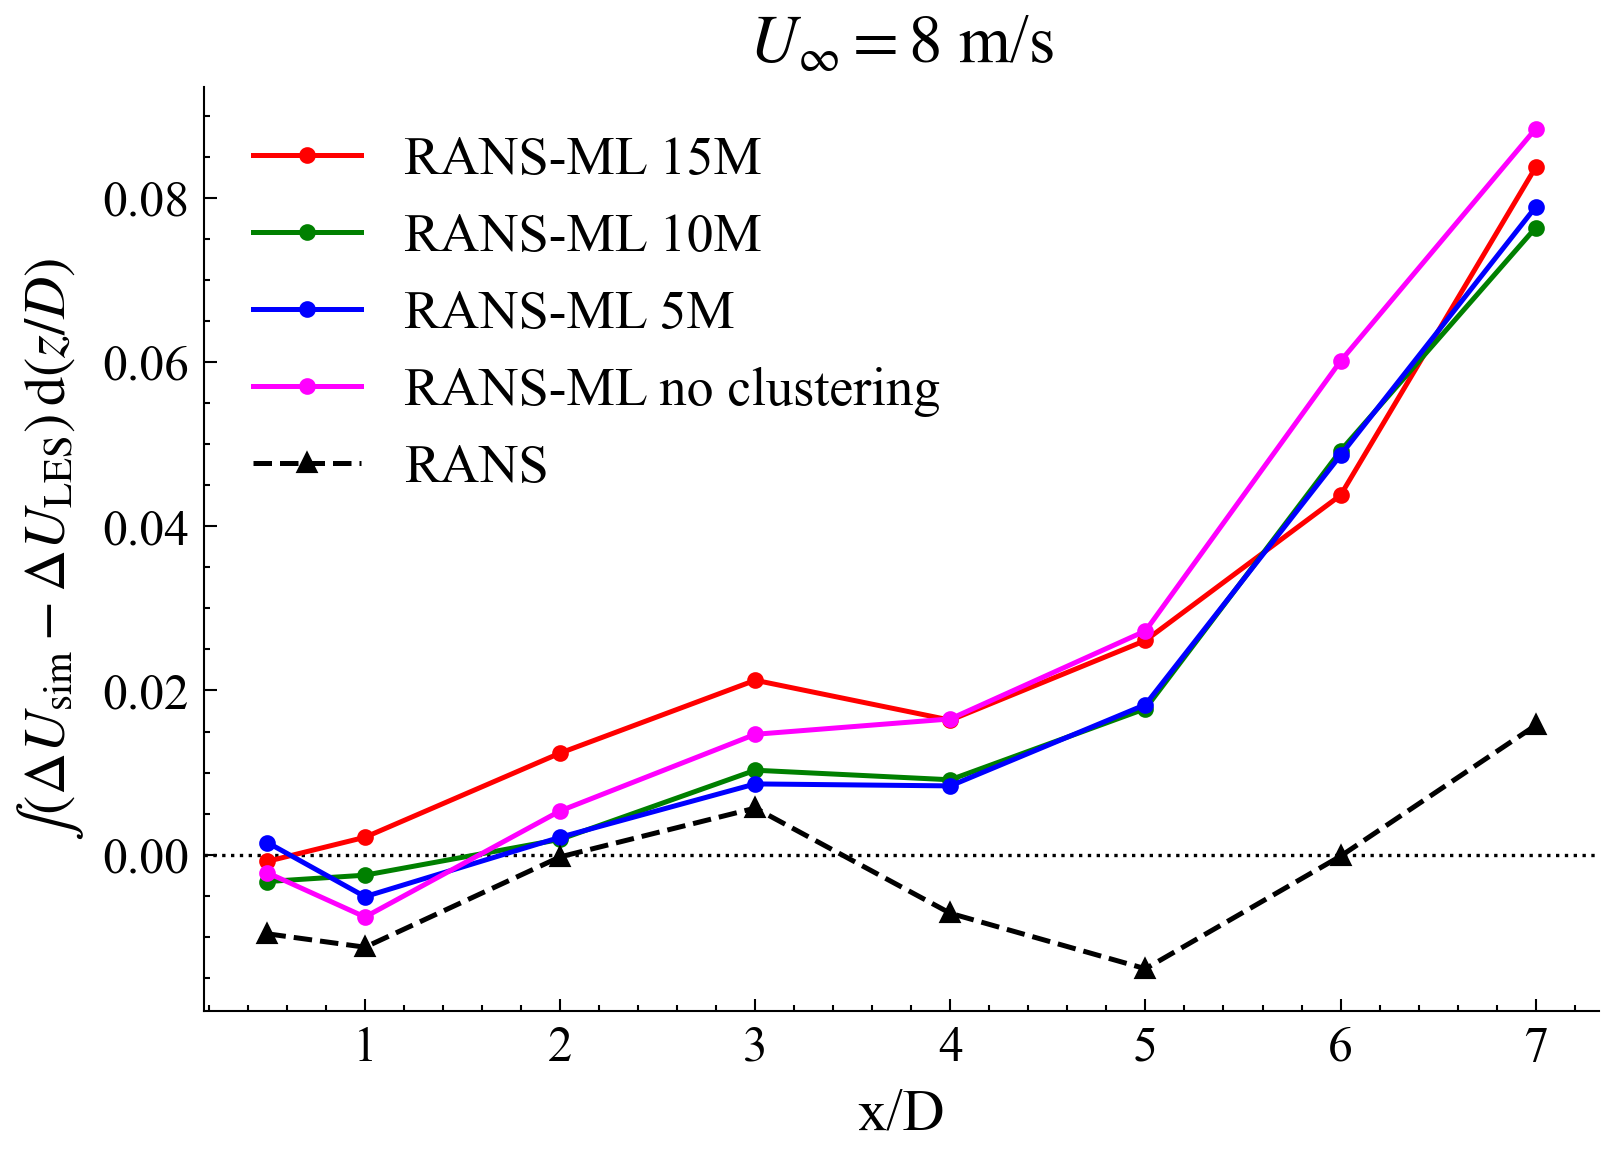
\includegraphics[width=\textwidth]{results/img/ml_results/8ms/integral_deficit_difference.png}
        \caption{}
        \label{fig:integral_8ms}
    \end{subfigure}
    \hfill
    \begin{subfigure}{0.32\textwidth}
        \centering
        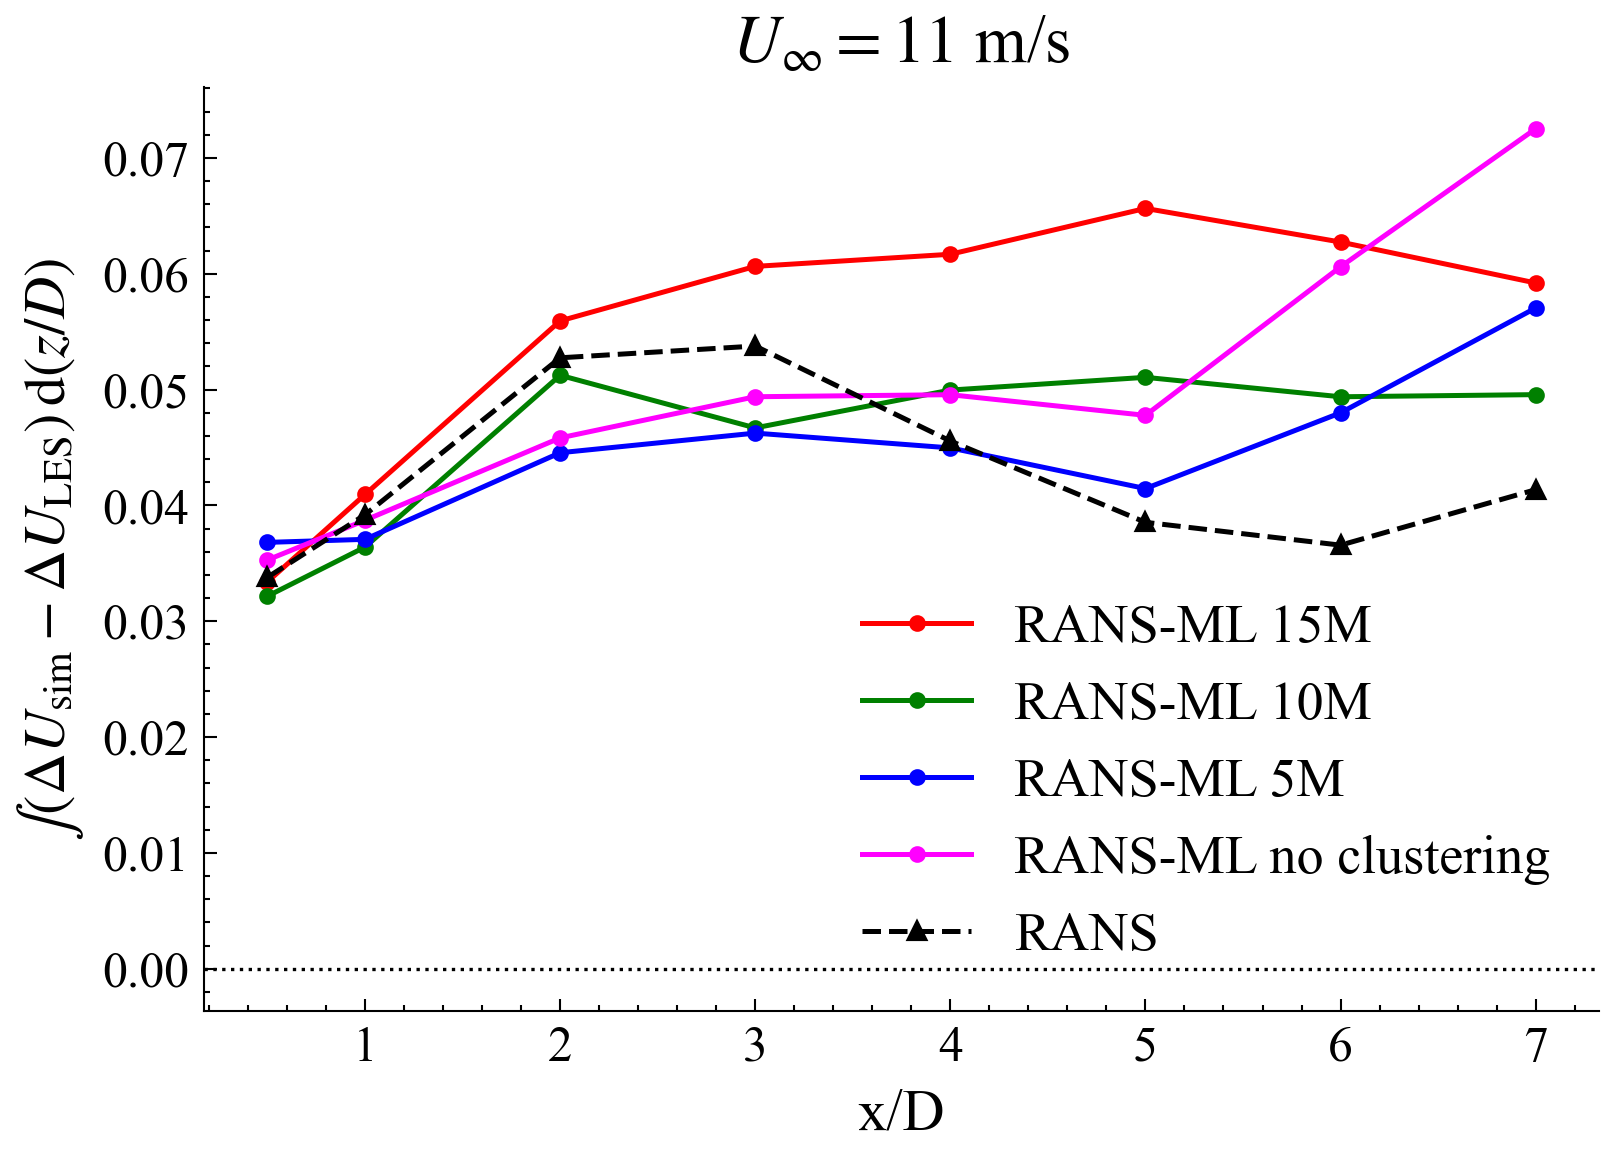
\includegraphics[width=\textwidth]{results/img/ml_results/11ms/integral_deficit_difference.png}
        \caption{}
        \label{fig:integral_11ms}
    \end{subfigure}
    \hfill
    \begin{subfigure}{0.32\textwidth}
        \centering
        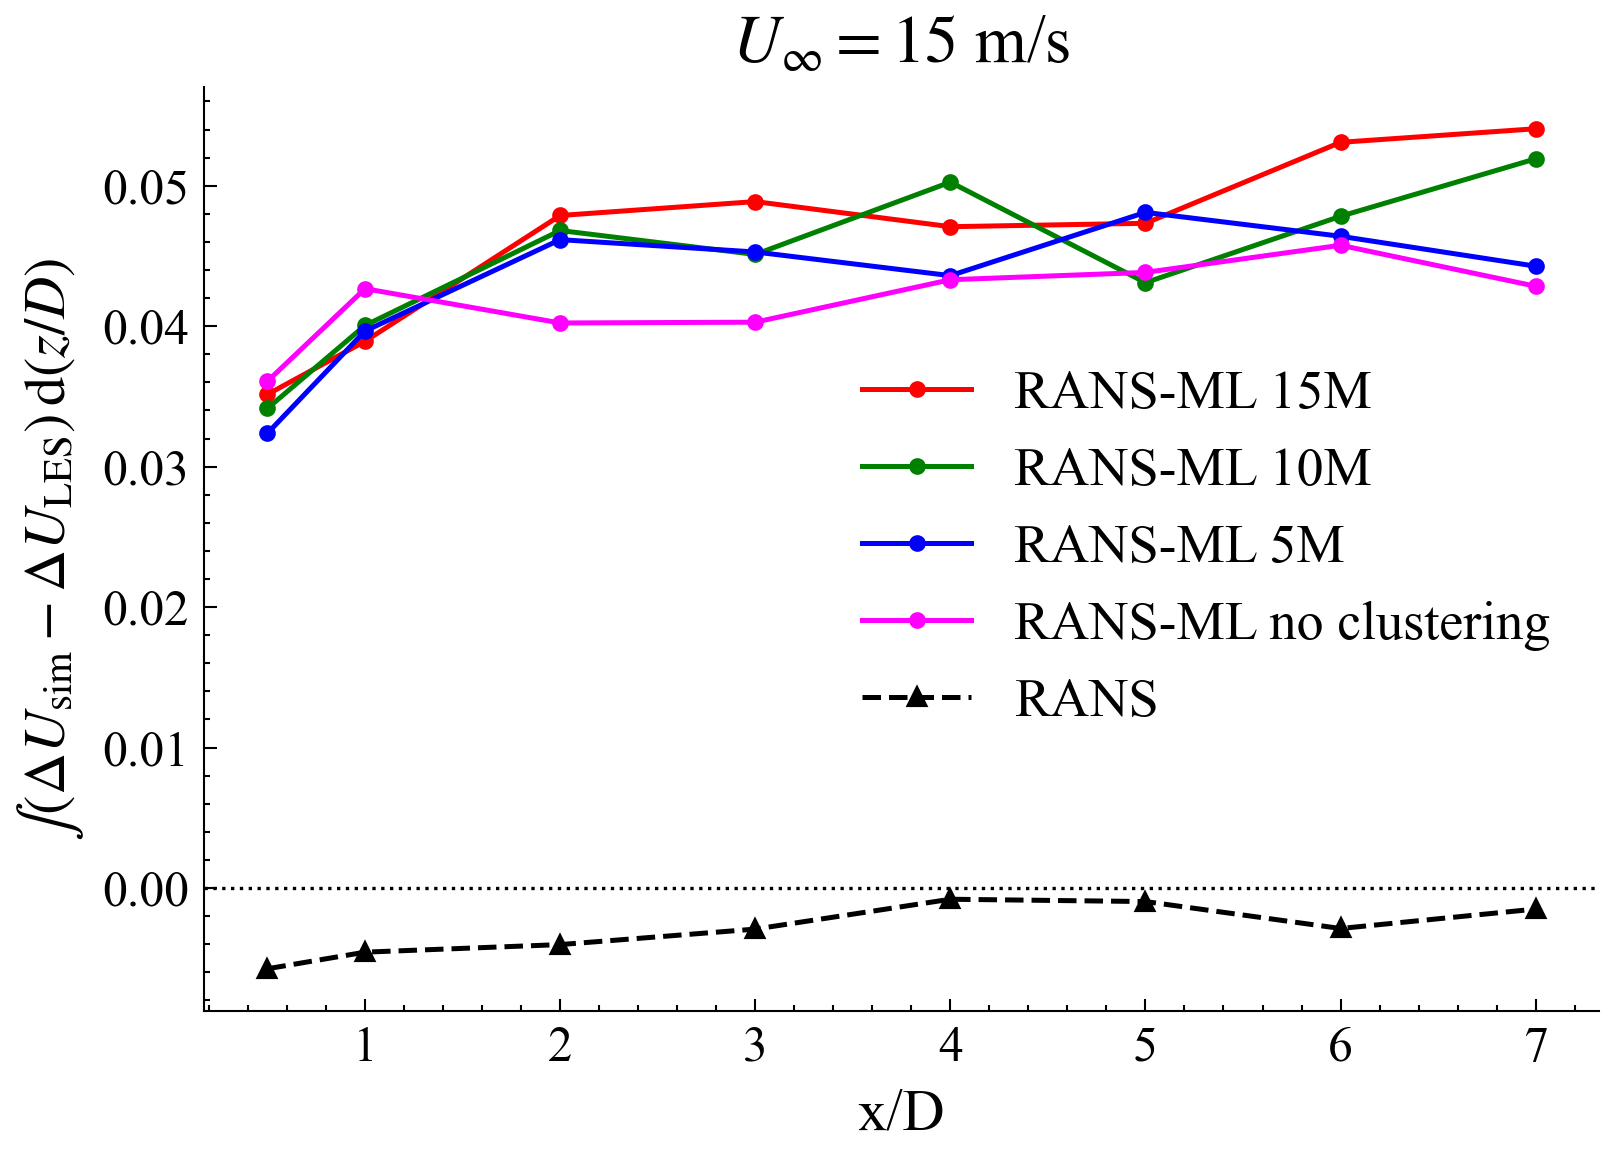
\includegraphics[width=\textwidth]{results/img/ml_results/15ms/integral_deficit_difference.png}
        \caption{}
        \label{fig:integral_15ms}
    \end{subfigure}
    \caption{Signed integral of the velocity-deficit difference with respect to the LES reference, Eq.~\ref{eq:integral_deficit_difference}, as a function of the streamwise distance, for the RANS-ML models on grids of different resolution and for the standard RANS model: (a) $U_\infty=8\,\mathrm{m/s}$, (b) $U_\infty=11\,\mathrm{m/s}$, (c) $U_\infty=15\,\mathrm{m/s}$.}
    \label{fig:integral_deficit_difference}
\end{figure}
For all three inflow velocities the standard RANS model exhibits a large and persistent positive offset throughout the wake, confirming a systematic overestimation of the velocity deficit and an excessively slow wake recovery. In contrast, all the RANS-ML configurations remain close to zero along the whole streamwise extent, even at the inflow conditions ($8$ and $15\,\mathrm{m/s}$) that were not part of the training set. This demonstrates that the learned eddy-viscosity correction is not tied to the specific velocity it was trained on but generalises across different inflow conditions, which is a key requirement for its application to wind farm flows where the operating wind speed varies in time. This is the central evidence supporting the single-case-to-many premise of the methodology: a closure calibrated on one operating point reproduces the LES wake recovery across the inflow envelope, with no retraining and no case-specific tuning.

To assess not only the capability of the model to predict the velocity field but also to investigate its ability to capture the dynamic effects on the wind turbine (and the relative power production), the predicted forces are reported here together with the predicted $C_p$ and $C_t$ values.
\begin{figure}
    \centering
    \begin{subfigure}{0.49\textwidth}
        \centering
        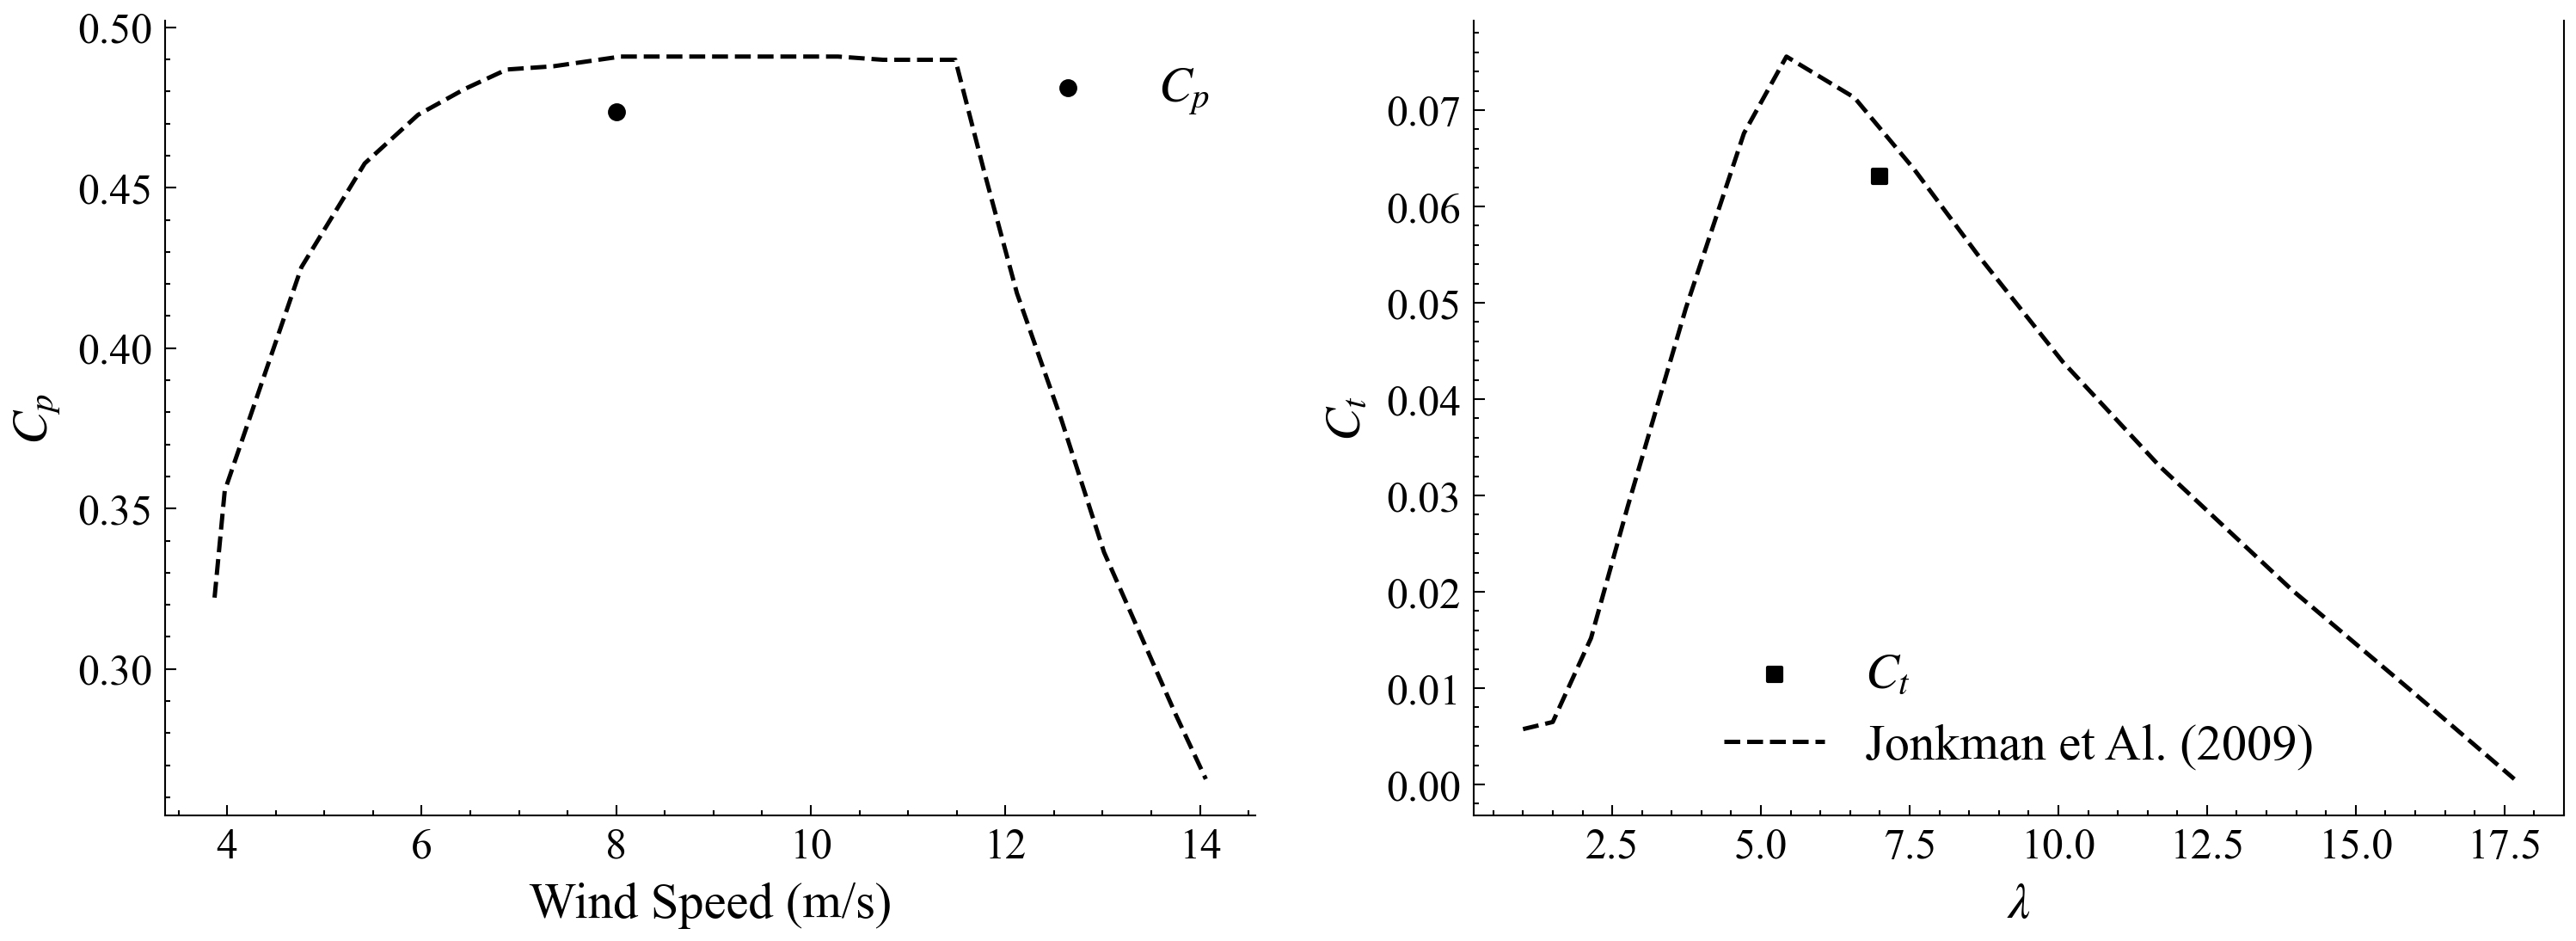
\includegraphics[width=\textwidth]{results/img/forces_cp_ct.png}
        \caption{}
        \label{fig:cp_ct_profile}
    \end{subfigure}
    \hfill
    \begin{subfigure}{0.49\textwidth}
        \centering
        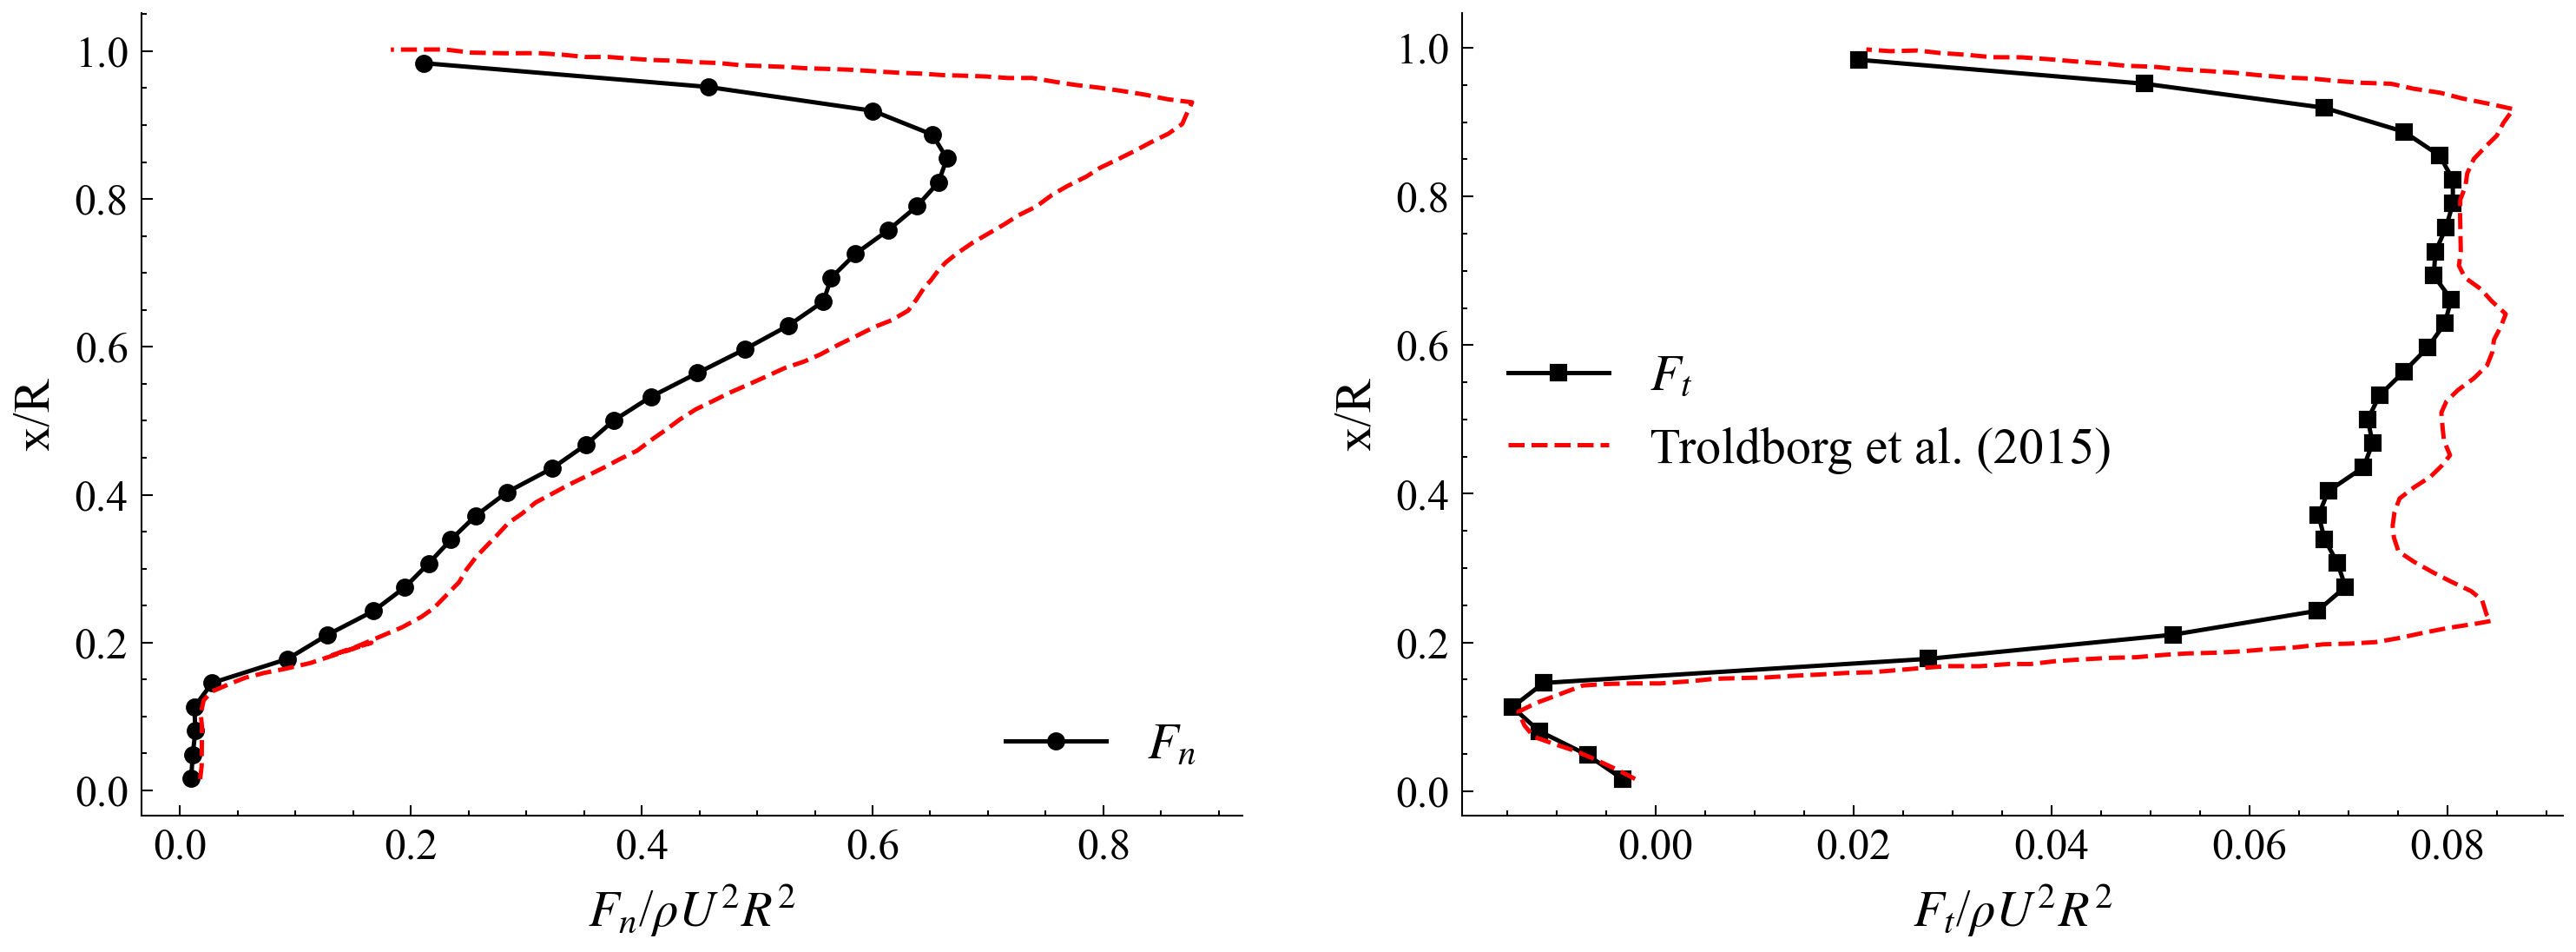
\includegraphics[width=\textwidth]{results/img/forces_profile.png}
        \caption{}
        \label{fig:forces_profile}
    \end{subfigure}
    \caption{ML-based RANS model results on the predicted forces and power coefficients: (a) $C_p$ and $C_t$ profiles, (b) force profiles.}
\end{figure}
The predicted forces show good agreement with the reference curves, with a slight underestimation of the overall forces and coefficients. A small deviation in terms of power production can be noted at the $C_p$ corresponding point; this is partly due to the fact that the reference curves refer to an isolated turbine configuration, whereas the ML-based RANS model is applied to a turbine operating in a turbulent ABL and affected by the presence of the ground. Overall, the predicted forces and power coefficients remain in accordance with the reference curves, demonstrating the capability of the ML-based RANS model to predict not only the velocity wake field but also the dynamic effects on the wind turbine and thus its power production, which is a key aspect for wind farm applications.
%%%conclusions
\section{Conclusions}
\label{sec:conclusions}

This work presented a CFD-ML methodology to build a turbulence closure aimed at improving the fidelity of
RANS simulations of HAWT wakes while keeping the
computational cost compatible with wind farm applications. The ML
module is used to define the turbulence model itself, by
learning the eddy-viscosity correction required to reproduce
high-fidelity LES statistics.

A LES of the NREL-5MW turbine operating in a turbulent atmospheric
boundary layer was used to generate the reference data. An
LES-equivalent eddy viscosity $\nu_{t,eq}$ was extracted by projecting
the deviatoric LES stress onto the Boussinesq form, and a Multi-Layer
Perceptron was trained to predict the local correction
$\Delta\nu_t = \nu_{t,eq} - \nu_{t,\mathrm{RANS}}$ with respect to the
RANS baseline. A K-means clustering algorithm was employed to segment
the domain into physically distinct flow regions, moving the prediction
from a cell-wise to a region-aware basis, and the resulting closure was
embedded into a modified OpenFOAM PIMPLE solver to be used in a fully
predictive setting. The main findings can be summarised as follows.

\begin{itemize}
    \item The clustering identified seven physically meaningful flow
    regions, separating the undisturbed flow from the
    inlet/ABL-affected, near-wake, mixing/breakdown and far-wake regions,
    consistently with the underlying flow physics.

    \item The trained network reproduced the LES-equivalent eddy
    viscosity with a validation $R^2 = 0.9952$
    ($RMSE = 0.2635$, $MAE = 0.1797$ in physical space), confirming that the learned correction drastically
    reduces the discrepancy with the LES-equivalent closure.

    \item The comparison with an equivalent network trained without
    clustering showed that the clustered model attains slightly better
    metrics across the board ($R^2 = 0.9952$ against $0.9950$, with lower
    $RMSE$ and $MAE$), reflecting a better reconstruction of the data
    variance. The benefit of clustering is
    most evident in the near-terrain region, where the clustered model
    is markedly more consistent with the LES reference, since it is able
    to learn separately the distinct near-wall and free-stream flow
    regimes.

    \item Once embedded in the solver, the ML-based RANS model
    consistently outperformed the standard RANS model in both the near-
    and far-wake. On the fine grid the model strongly improved the
    near-wake prediction, especially in the upper part of the wake,
    while slightly underestimating the deficit in the lower near-wake
    and overestimating it in the far-wake after the wake breakdown.

    \item The most relevant result for practical applications was
    obtained on the ultra-coarse grids: the model retained its improved
    near-wake prediction while also accurately reproducing the
    post-breakdown far-wake recovery, at a computational cost about
    $1.25$ times lower than the reference LES on the
    $\sim\!4.2\times10^6$ cells grid. Since downstream turbines are
    typically located in the far-wake of the upstream machines, this
    combination of far-wake accuracy and reduced cost is precisely what
    is required for wind farm layout and energy-yield studies.

    \item Although trained on a single inflow velocity
    ($U_\infty = 11\,\mathrm{m/s}$), the closure generalised well to the
    unseen $8$ and $15\,\mathrm{m/s}$ conditions: a scalar metric based on
    the integral of the velocity-deficit difference with respect to the
    LES showed that, at all three inflow velocities, the standard RANS
    model systematically overestimates the wake deficit while every
    RANS-ML configuration remains close to the LES reference throughout
    the wake.

    \item Beyond the velocity field, the model also reproduced the rotor
    forces and the $C_p$/$C_t$ coefficients in good agreement with the
    reference curves, with only a slight underestimation partly
    attributable to the more realistic ABL and ground-affected operating
    conditions, demonstrating its ability to capture the aerodynamic
    loading and the associated power production.
\end{itemize}

Two aspects deserve to be stated clearly, so that they are not mistaken
for weaknesses. First, training on a single operating condition and a
compact dataset is a deliberate design choice and the very premise of the
methodology, not a constraint: the aim is to calibrate the closure once,
on an affordable amount of high-fidelity data, and to reuse it across the
operating envelope, as the transfer to the unseen $8$ and
$15\,\mathrm{m/s}$ conditions and to coarser grids confirms. The mild
train/validation gap is the expected signature of this compact
calibration and, as shown, it does not degrade the out-of-sample
performance. Second, by construction the model remains a scalar
eddy-viscosity closure: it corrects the magnitude and distribution of
$\nu_t$ to reproduce the LES mixing, but does not represent the
Reynolds-stress anisotropy, a deliberate trade-off that keeps the closure
directly embeddable in standard solvers.

Genuine residual limitations remain and outline the path forward. A
residual underestimation bias persists in the far-upstream inflow region,
inherited from the synthetic inlet boundary condition, and the fine-grid
configuration still overestimates the far-wake deficit. Future work will
therefore enlarge the training dataset to multiple inflow velocities,
turbulence intensities and thermal-stability conditions, so as to broaden
the validated operating range and further tighten the closure; it will
explore tensorial, anisotropy-aware corrections to overcome the scalar
limitation; and it will extend the methodology to multi-turbine
configurations to assess wake-interaction effects. The compactness and
the reduced cost of the proposed data-driven closure also make it a
promising candidate for future real-time wind farm monitoring and control
applications, where accurate yet inexpensive representations of the wake
field are essential.


%%% bibliography
\bibliographystyle{unsrt}
\bibliography{bib/ref.bib}
\end{document}
